\documentclass[12pt,a4paper]{article}

\usepackage[a4paper,left=2.7cm,right=2.7cm,top=2.6cm,bottom=2.6cm]{geometry}
\usepackage[utf8]{inputenc}
\usepackage[T1]{fontenc}
\usepackage[brazilian]{babel}
\usepackage{lmodern}
\usepackage{microtype}
\usepackage{amsmath,amssymb}
\usepackage{graphicx}
\usepackage{booktabs}
\usepackage{float}
\usepackage{pdflscape}
\usepackage{caption}
\usepackage{subcaption}
\usepackage{setspace}
\usepackage{xcolor}
\usepackage{titlesec}
\usepackage{fancyhdr}
\usepackage[hidelinks]{hyperref}

\definecolor{bndesblue}{HTML}{2A4089}
\definecolor{bndesgreen}{HTML}{127D3E}
\definecolor{lightblue}{HTML}{EEF2FA}
\definecolor{midgray}{HTML}{666666}

\graphicspath{{../analysis/}}
\captionsetup{font=small,labelfont={bf,color=bndesblue},justification=justified,singlelinecheck=false}
\setlength{\parindent}{1.2cm}
\setlength{\parskip}{0.15em}
\onehalfspacing

\titleformat{\section}{\Large\bfseries\color{bndesblue}}{\thesection}{0.65em}{}
\titleformat{\subsection}{\large\bfseries\color{bndesgreen}}{\thesubsection}{0.65em}{}
\titleformat{\subsubsection}{\normalsize\bfseries\color{bndesblue}}{\thesubsubsection}{0.65em}{}

\pagestyle{fancy}
\setlength{\headheight}{14pt}
\fancyhf{}
\fancyhead[L]{\small\color{midgray}Avaliação dos efeitos do FUST sobre empresas}
\fancyhead[R]{\small\color{midgray}Produto 3}
\fancyfoot[C]{\thepage}
\renewcommand{\headrulewidth}{0.35pt}

\newcommand{\ATT}{\operatorname{ATT}}
\newcommand{\E}{\mathbb{E}}
\newcommand{\pct}[1]{\ensuremath{#1\%}}
\newcommand{\figurenote}[1]{\par\vspace{0.3em}{\footnotesize\setstretch{1.05}\textit{Nota:} #1}}

\begin{document}
\hypersetup{pageanchor=false}

\begin{titlepage}
  \thispagestyle{empty}
  \vspace*{2.2cm}
  \noindent{\color{bndesgreen}\rule{\textwidth}{4pt}}\\[1.1cm]
  {\Huge\bfseries\color{bndesblue} Efeitos do apoio FUST sobre o\\[0.2em] desempenho das empresas\par}
  \vspace{0.8cm}
  {\Large Relatório de interpretação dos resultados\par}
  \vspace{0.35cm}
  {\large Produto 3\par}
  \vfill
  \begin{minipage}{0.88\textwidth}
    \colorbox{lightblue}{\parbox{0.83\textwidth}{
      \setstretch{1.25}
      Este relatório sistematiza e interpreta os 19 resultados finais disponíveis na pasta
      \texttt{analysis}: o balanceamento da amostra, três estudos de evento, três análises de
      heterogeneidade e doze figuras de robustez. A interpretação se baseia exclusivamente nos
      dados, códigos e resultados do Produto 3.
    }}
  \end{minipage}
  \vfill
  {\large Agosto de 2026\par}
  \vspace{1cm}
  \noindent{\color{bndesblue}\rule{\textwidth}{1.2pt}}
\end{titlepage}

\hypersetup{pageanchor=true}
\pagenumbering{roman}
\tableofcontents
\clearpage
\pagenumbering{arabic}

% -----------------------------------------------------------------------------
\section{Metodologia}

O objetivo da avaliação é estimar como o primeiro apoio do Fundo de Universalização dos
Serviços de Telecomunicações (FUST) altera a trajetória das empresas beneficiárias. A unidade
de análise é o CNPJ-raiz. O tratamento ocorre no ano do primeiro apoio e permanece ativo nos
anos seguintes. Há duas coortes tratadas, em 2024 e 2025, e o grupo de comparação é formado por
empresas que não receberam apoio do FUST no período observado.

A estratégia empírica combina pareamento e diferenças-em-diferenças com adoção escalonada. O
pareamento aproxima empresas apoiadas e não apoiadas em características observadas antes do
tratamento; a etapa de diferenças-em-diferenças compara, então, a mudança dos desfechos nas
tratadas com a mudança observada nos controles. Essa combinação reduz diferenças de composição
em níveis e usa a evolução temporal dos controles para construir o contrafactual das empresas
beneficiárias.

\subsection{Construção da amostra comparável}

A especificação principal utiliza pareamento 1:1, sem reposição e realizado separadamente por
coorte. A distância de Mahalanobis é calculada com seis características pré-FUST: idade da
empresa, proporção de trabalhadores com ensino superior, tempo médio de emprego, idade média dos
trabalhadores, proporção de homens e proporção de trabalhadores pretos ou pardos. O pareamento é
exato pela divisão da CNAE e impõe coerência entre a classificação setorial observada nas bases
do BNDES e da RAIS. A amostra oficial também exige presença depois do tratamento e observação na
janela temporal pertinente. O resultado é uma amostra de 224 empresas tratadas e 224 controles.

\subsection{Desenho de diferenças-em-diferenças}

A estimação principal segue Callaway--Sant'Anna para tratamentos escalonados. Para cada coorte
$g$ e ano $t$, estima-se
\begin{equation}
  \ATT(g,t)=\E\!\left[Y_{it}(1)-Y_{it}(0)\mid G_i=g\right],
\end{equation}
em que $G_i$ é o ano do primeiro apoio. As empresas nunca tratadas formam o grupo de controle. O
estimador utilizado é duplamente robusto e admite painel não balanceado. Os efeitos por tempo
relativo são agregações dos $\ATT(g,t)$ para observações com $e=t-g$:
\begin{equation}
  \theta(e)=\sum_{g:g+e\in\mathcal{T}} w_{g,e}\,\ATT(g,g+e),
\end{equation}
com $e=-1$ normalizado a zero. A janela vai de quatro anos antes a um ano depois do apoio. Como a
base termina em 2025, o coeficiente em $e=1$ é identificado apenas pela coorte de 2024; o efeito
contemporâneo, $e=0$, usa as duas coortes. O ATT médio apresentado nas figuras é a média ponderada
dos efeitos pós-tratamento disponíveis.

Os intervalos de confiança pontuais são de 95\%. Os estudos de evento permitem avaliar a
dinâmica dos efeitos e inspecionar o comportamento pré-tratamento. A interpretação causal requer
que, na ausência do FUST, tratadas e controles apresentassem tendências paralelas, além da
ausência de antecipação e de efeitos do tratamento de uma empresa sobre os resultados de outra.

% -----------------------------------------------------------------------------
\section{Dados}

A análise combina os registros das operações do FUST com os microdados da Relação Anual de
Informações Sociais (RAIS). Os registros do FUST identificam a empresa, a data do primeiro apoio,
a modalidade, o porte BNDES e o número de subcréditos. A RAIS fornece os vínculos formais ativos e as
remunerações, agregados ao CNPJ-raiz e ao ano. O painel cobre 2020--2025.

Três desfechos são avaliados:
\begin{itemize}
  \item \textbf{Emprego}: $\log(1+\text{número de vínculos formais ativos})$;
  \item \textbf{Massa salarial}: $\log(1+\text{soma das remunerações dos vínculos ativos})$;
  \item \textbf{Salário médio}: logaritmo da remuneração média por vínculo ativo.
\end{itemize}

Os efeitos estimados estão, portanto, em pontos de log. Para facilitar a leitura, um coeficiente
$\widehat\beta$ pode ser convertido em variação percentual por
$100\,[\exp(\widehat\beta)-1]$. Essa transformação é usada nas interpretações a seguir. Efeitos
em emprego, massa salarial e salário médio não devem ser tratados como uma decomposição contábil
exata: os dois primeiros desfechos usam $\log(1+x)$, a disponibilidade de observações pode variar
entre resultados e os ATTs são agregados por coorte e tempo relativo.

% -----------------------------------------------------------------------------
\section{Diferença de média}

A Tabela~\ref{tab:balance} compara as empresas tratadas com o universo de controles elegíveis e
com os controles pareados. Antes do pareamento, há diferenças relevantes em tempo de emprego,
idade dos trabalhadores e composição racial. As tratadas têm, em média, vínculos mais recentes,
trabalhadores mais jovens e menor proporção de pretos ou pardos. O pareamento elimina essas três
diferenças e também mantém equilibrada a proporção de homens.

O balanceamento, contudo, não é completo. Depois do pareamento, as tratadas permanecem mais
antigas e apresentam maior proporção de trabalhadores com ensino superior; as diferenças são
estatisticamente significativas e, nessas duas covariadas, maiores do que na comparação com o
universo de controles. Isso não invalida automaticamente o desenho de diferenças-em-diferenças,
que permite diferenças fixas de nível, mas reforça a importância de verificar pré-tendências e
de considerar a robustez com controles pré-FUST interagidos com ano.

\begin{landscape}
\begin{table}[H]
\centering
\caption{Balanceamento antes e depois do pareamento}
\label{tab:balance}
\small
\setlength{\tabcolsep}{6pt}
\begin{tabular}{lrrrrr}
\toprule
Covariada & Tratamento & Controle completo & Controle pareado & Dif. (1)--(2) & Dif. (1)--(3) \\
\midrule
Idade da empresa & 14,071 & 12,910 & 12,442 & 1,161*** & 1,629*** \\
Proporção com ensino superior & 0,273 & 0,266 & 0,222 & 0,007 & 0,051** \\
Tempo médio de emprego & 34,404 & 45,725 & 33,074 & $-11,321$*** & 1,330 \\
Idade média dos trabalhadores & 31,512 & 39,535 & 31,572 & $-8,024$*** & $-0,060$ \\
Proporção de homens & 0,684 & 0,687 & 0,683 & $-0,004$ & 0,001 \\
Proporção de pretos (pardos + negros) & 0,052 & 0,081 & 0,054 & $-0,029$*** & $-0,002$ \\
\midrule
Número de empresas (CNPJ-raiz) & 224 & 20.337 & 224 & & \\
\bottomrule
\end{tabular}
\vspace{0.5em}

\begin{minipage}{0.92\linewidth}
\footnotesize\setstretch{1.05}\textit{Nota:} a coluna ``controle completo'' contém empresas não
apoiadas elegíveis nas mesmas coortes e nos mesmos municípios das tratadas. A coluna ``controle
pareado'' contém as empresas selecionadas para a especificação principal. Há 195 municípios
tratados. *** $p<0{,}01$; ** $p<0{,}05$; * $p<0{,}10$.
\end{minipage}
\end{table}
\end{landscape}

% -----------------------------------------------------------------------------
\section{Modelo}

O modelo empírico pode ser representado, apenas para fins expositivos, por um estudo de evento
com efeitos fixos de empresa e de ano:
\begin{equation}
  Y_{it}=\alpha_i+\lambda_t+\sum_{e\neq-1}\beta_e
  \mathbf{1}\{t-G_i=e\}+\varepsilon_{it}.
  \label{eq:event}
\end{equation}
Os $\beta_e$ medem diferenças entre tratadas e controles em relação ao ano imediatamente anterior
ao apoio. A Equação~\eqref{eq:event} ajuda a interpretar as figuras, mas os resultados principais
não são obtidos por uma regressão TWFE convencional. Eles são construídos a partir de ATTs por
coorte e ano, evitando comparações inadequadas entre unidades já tratadas e unidades tratadas em
outros momentos.

Há três parâmetros de interesse. Primeiro, $\theta(0)$ mede o efeito no próprio ano do primeiro
apoio. Segundo, $\theta(1)$ mede o efeito no ano seguinte, disponível apenas para a coorte de
2024. Terceiro, o ATT pós-tratamento resume os dois horizontes. Os coeficientes anteriores ao
apoio não são efeitos do FUST; eles funcionam como diagnóstico de antecipação e de tendências
paralelas.

O estimando deve ser lido como efeito médio sobre as empresas apoiadas representadas na amostra
pareada e que satisfazem os critérios de disponibilidade de dados. Ele não identifica, sem
hipóteses adicionais, o efeito sobre todas as empresas brasileiras nem sobre empresas sem suporte
comparável. A curta janela pós-tratamento também restringe a análise aos impactos de curto prazo.

% -----------------------------------------------------------------------------
\section{Resultados}

\subsection{Síntese dos efeitos médios}

Os resultados principais apontam aumento de escala das empresas apoiadas. O ATT médio do log do
emprego é 0,225 (erro-padrão 0,053), equivalente a aproximadamente \pct{25,2}. Para a massa
salarial, o ATT é 0,362 (erro-padrão 0,138), ou cerca de \pct{43,6}. Ambos são positivos e
estatisticamente diferentes de zero a 5\%. Em contraste, o efeito sobre o salário médio é
$-0,012$ (erro-padrão 0,023), aproximadamente $-1,2\%$, e não é estatisticamente significativo.

\begin{table}[H]
\centering
\caption{Efeitos médios pós-tratamento na especificação principal}
\label{tab:main}
\begin{tabular}{lrrrr}
\toprule
Desfecho & ATT & Erro-padrão & IC 95\% (log) & Variação aproximada \\
\midrule
Emprego & 0,225*** & 0,053 & [0,121; 0,329] & +25,2\% \\
Massa salarial & 0,362*** & 0,138 & [0,092; 0,632] & +43,6\% \\
Salário médio & $-0,012$ & 0,023 & [$-0,056$; 0,033] & $-1,2\%$ \\
\bottomrule
\end{tabular}
\figurenote{Conversão percentual por $100[\exp(\widehat\beta)-1]$. Intervalos pontuais de 95\%.
*** indica significância a 1\%.}
\end{table}

O padrão sugere que o apoio está associado principalmente à expansão da atividade e do emprego,
e não a um aumento generalizado da remuneração média por trabalhador. Como emprego e massa
salarial crescem enquanto o salário médio permanece estável na especificação principal, a leitura
mais prudente é de expansão da folha por aumento do número de vínculos. A diferença de magnitude
entre os efeitos não deve ser interpretada como uma identidade contábil, pelos motivos descritos
na seção de dados.

\subsection{Os três estudos de evento}

\subsubsection{Emprego}

Antes do apoio, os coeficientes pontuais são próximos de zero e seus intervalos individuais
incluem zero. No ano do primeiro apoio, o efeito é 0,150, equivalente a aproximadamente
\pct{16,2}; no ano seguinte, sobe para 0,300, ou \pct{35,0}. A trajetória crescente indica que a
resposta do emprego se intensifica após a entrada no programa. Contudo, o teste conjunto de
pré-tendências rejeita a hipótese nula ($p=0{,}014$), o que recomenda cautela apesar do aspecto
visual favorável. A análise HonestDiD do apêndice avalia diretamente essa fragilidade.

\begin{figure}[p]
\centering
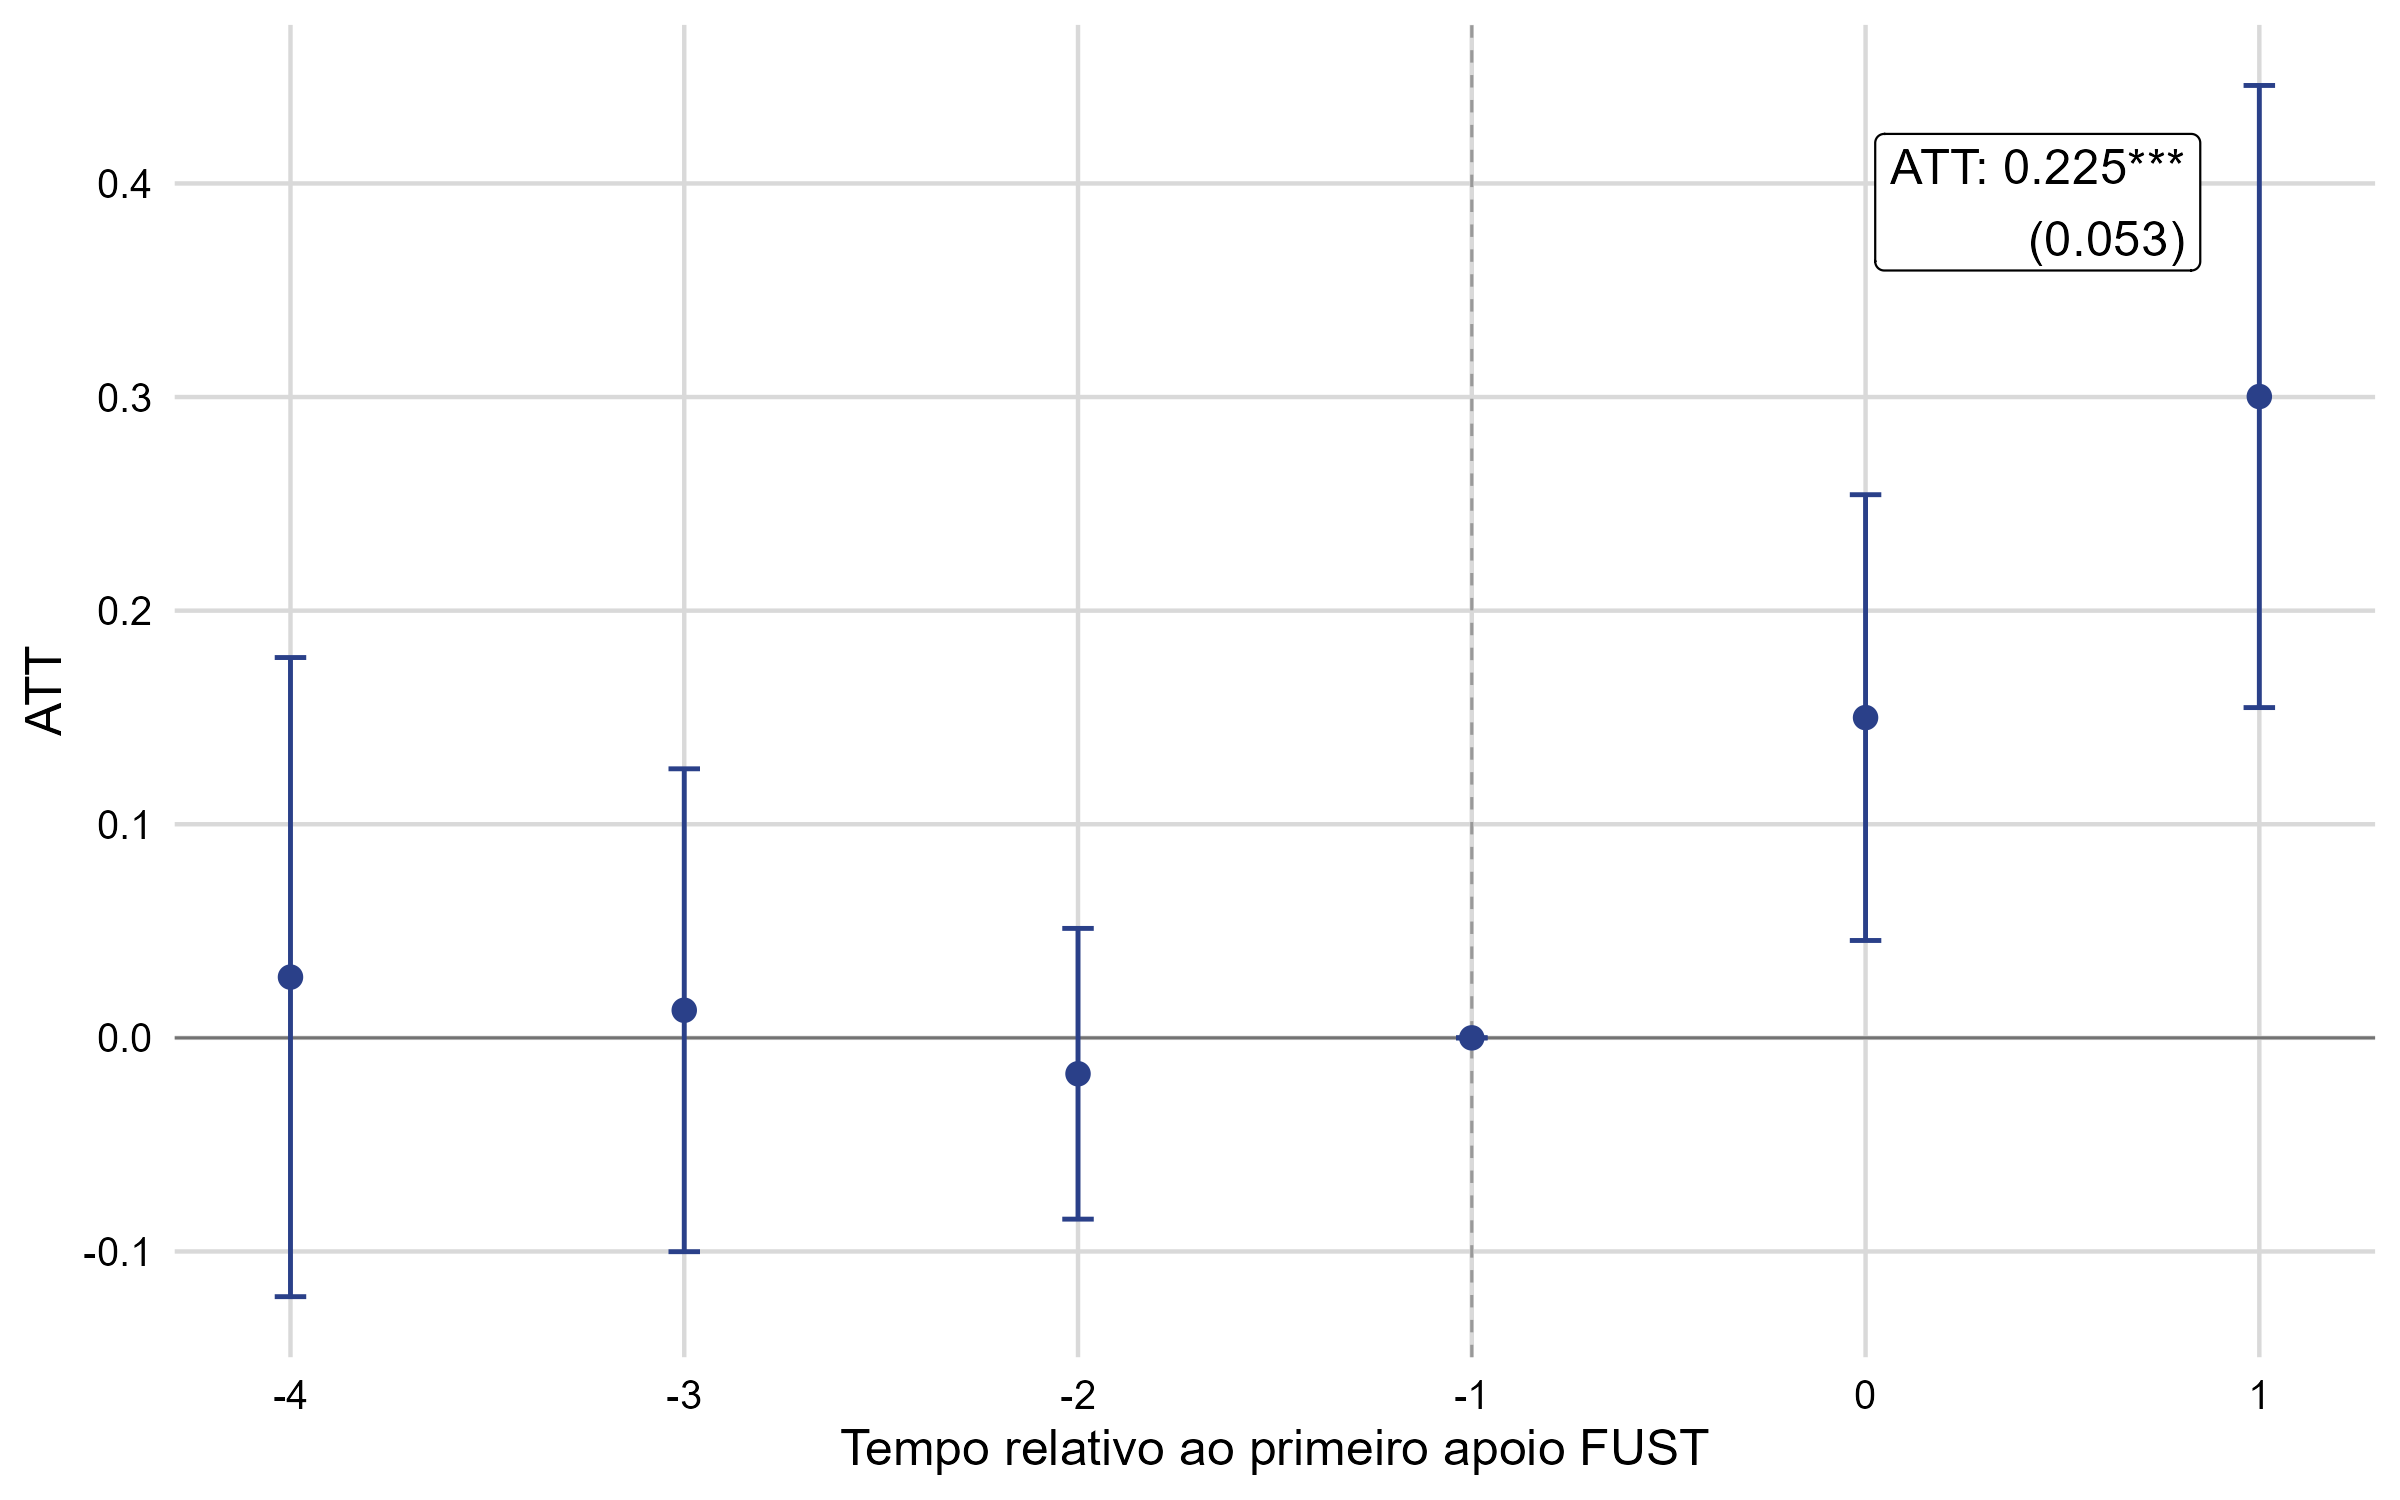
\includegraphics[width=0.96\textwidth]{Event study - CS - Log-emprego.png}
\caption{Estudo de evento: emprego}
\label{fig:es_emprego}
\figurenote{Estimador de Callaway--Sant'Anna. O período $e=-1$ é a referência. Pontos são ATTs por
tempo relativo e barras representam intervalos pontuais de 95\%.}
\end{figure}

\subsubsection{Massa salarial}

Os coeficientes anteriores ao tratamento oscilam em torno de zero e o teste conjunto não rejeita
pré-tendências nulas ($p=0{,}135$). O efeito é 0,276 no próprio ano do apoio, aproximadamente
\pct{31,8}, e 0,447 no ano seguinte, cerca de \pct{56,4}. A dinâmica acompanha a expansão do
emprego e também se torna mais intensa no segundo horizonte.

\begin{figure}[p]
\centering
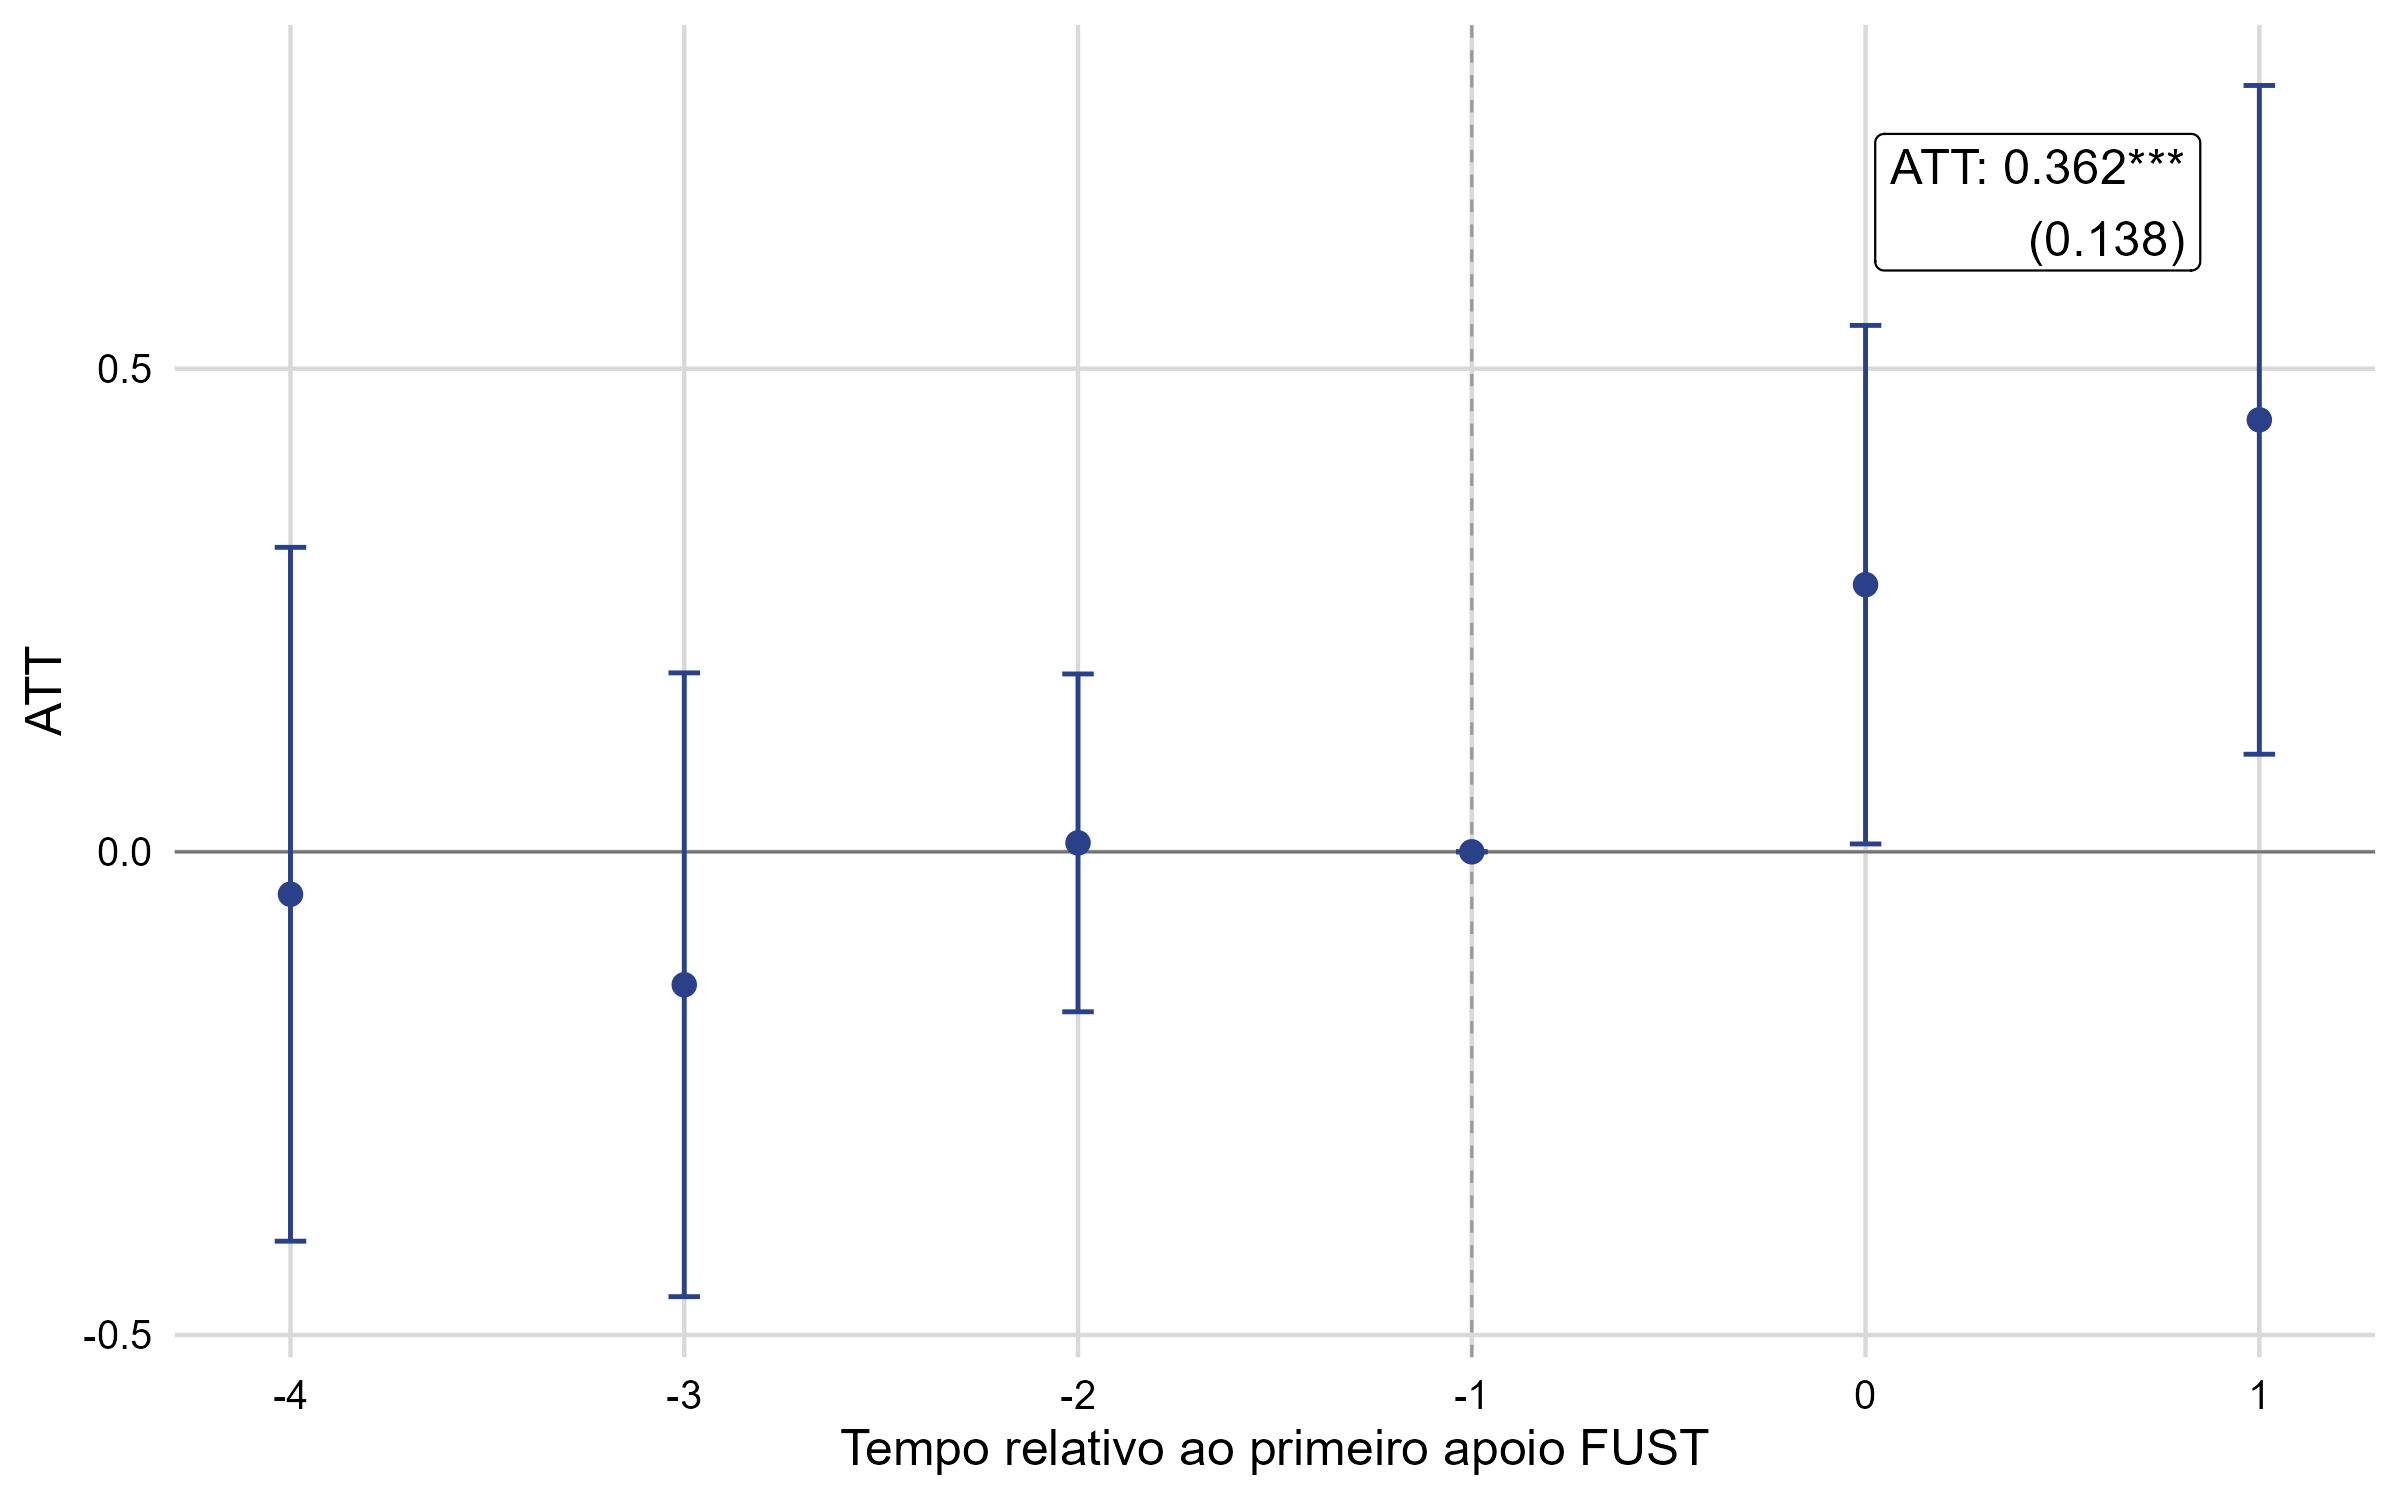
\includegraphics[width=0.96\textwidth]{Event study - CS - Log-massa-salarial.png}
\caption{Estudo de evento: massa salarial}
\label{fig:es_massa}
\figurenote{Estimador de Callaway--Sant'Anna. O período $e=-1$ é a referência. Pontos são ATTs por
tempo relativo e barras representam intervalos pontuais de 95\%.}
\end{figure}

\subsubsection{Salário médio}

Não há evidência de alteração do salário médio no ano do apoio ($-0,001$) ou no ano seguinte
($-0,022$). Os intervalos são compatíveis com efeitos positivos ou negativos modestos. O teste
conjunto de pré-tendências, entretanto, rejeita com força a hipótese nula ($p<0{,}001$), mesmo que
os intervalos pontuais dos três coeficientes pré-FUST incluam zero. Consequentemente, a conclusão
adequada é ausência de evidência robusta de aumento do salário médio, e não evidência definitiva
de efeito exatamente nulo.

\begin{figure}[p]
\centering
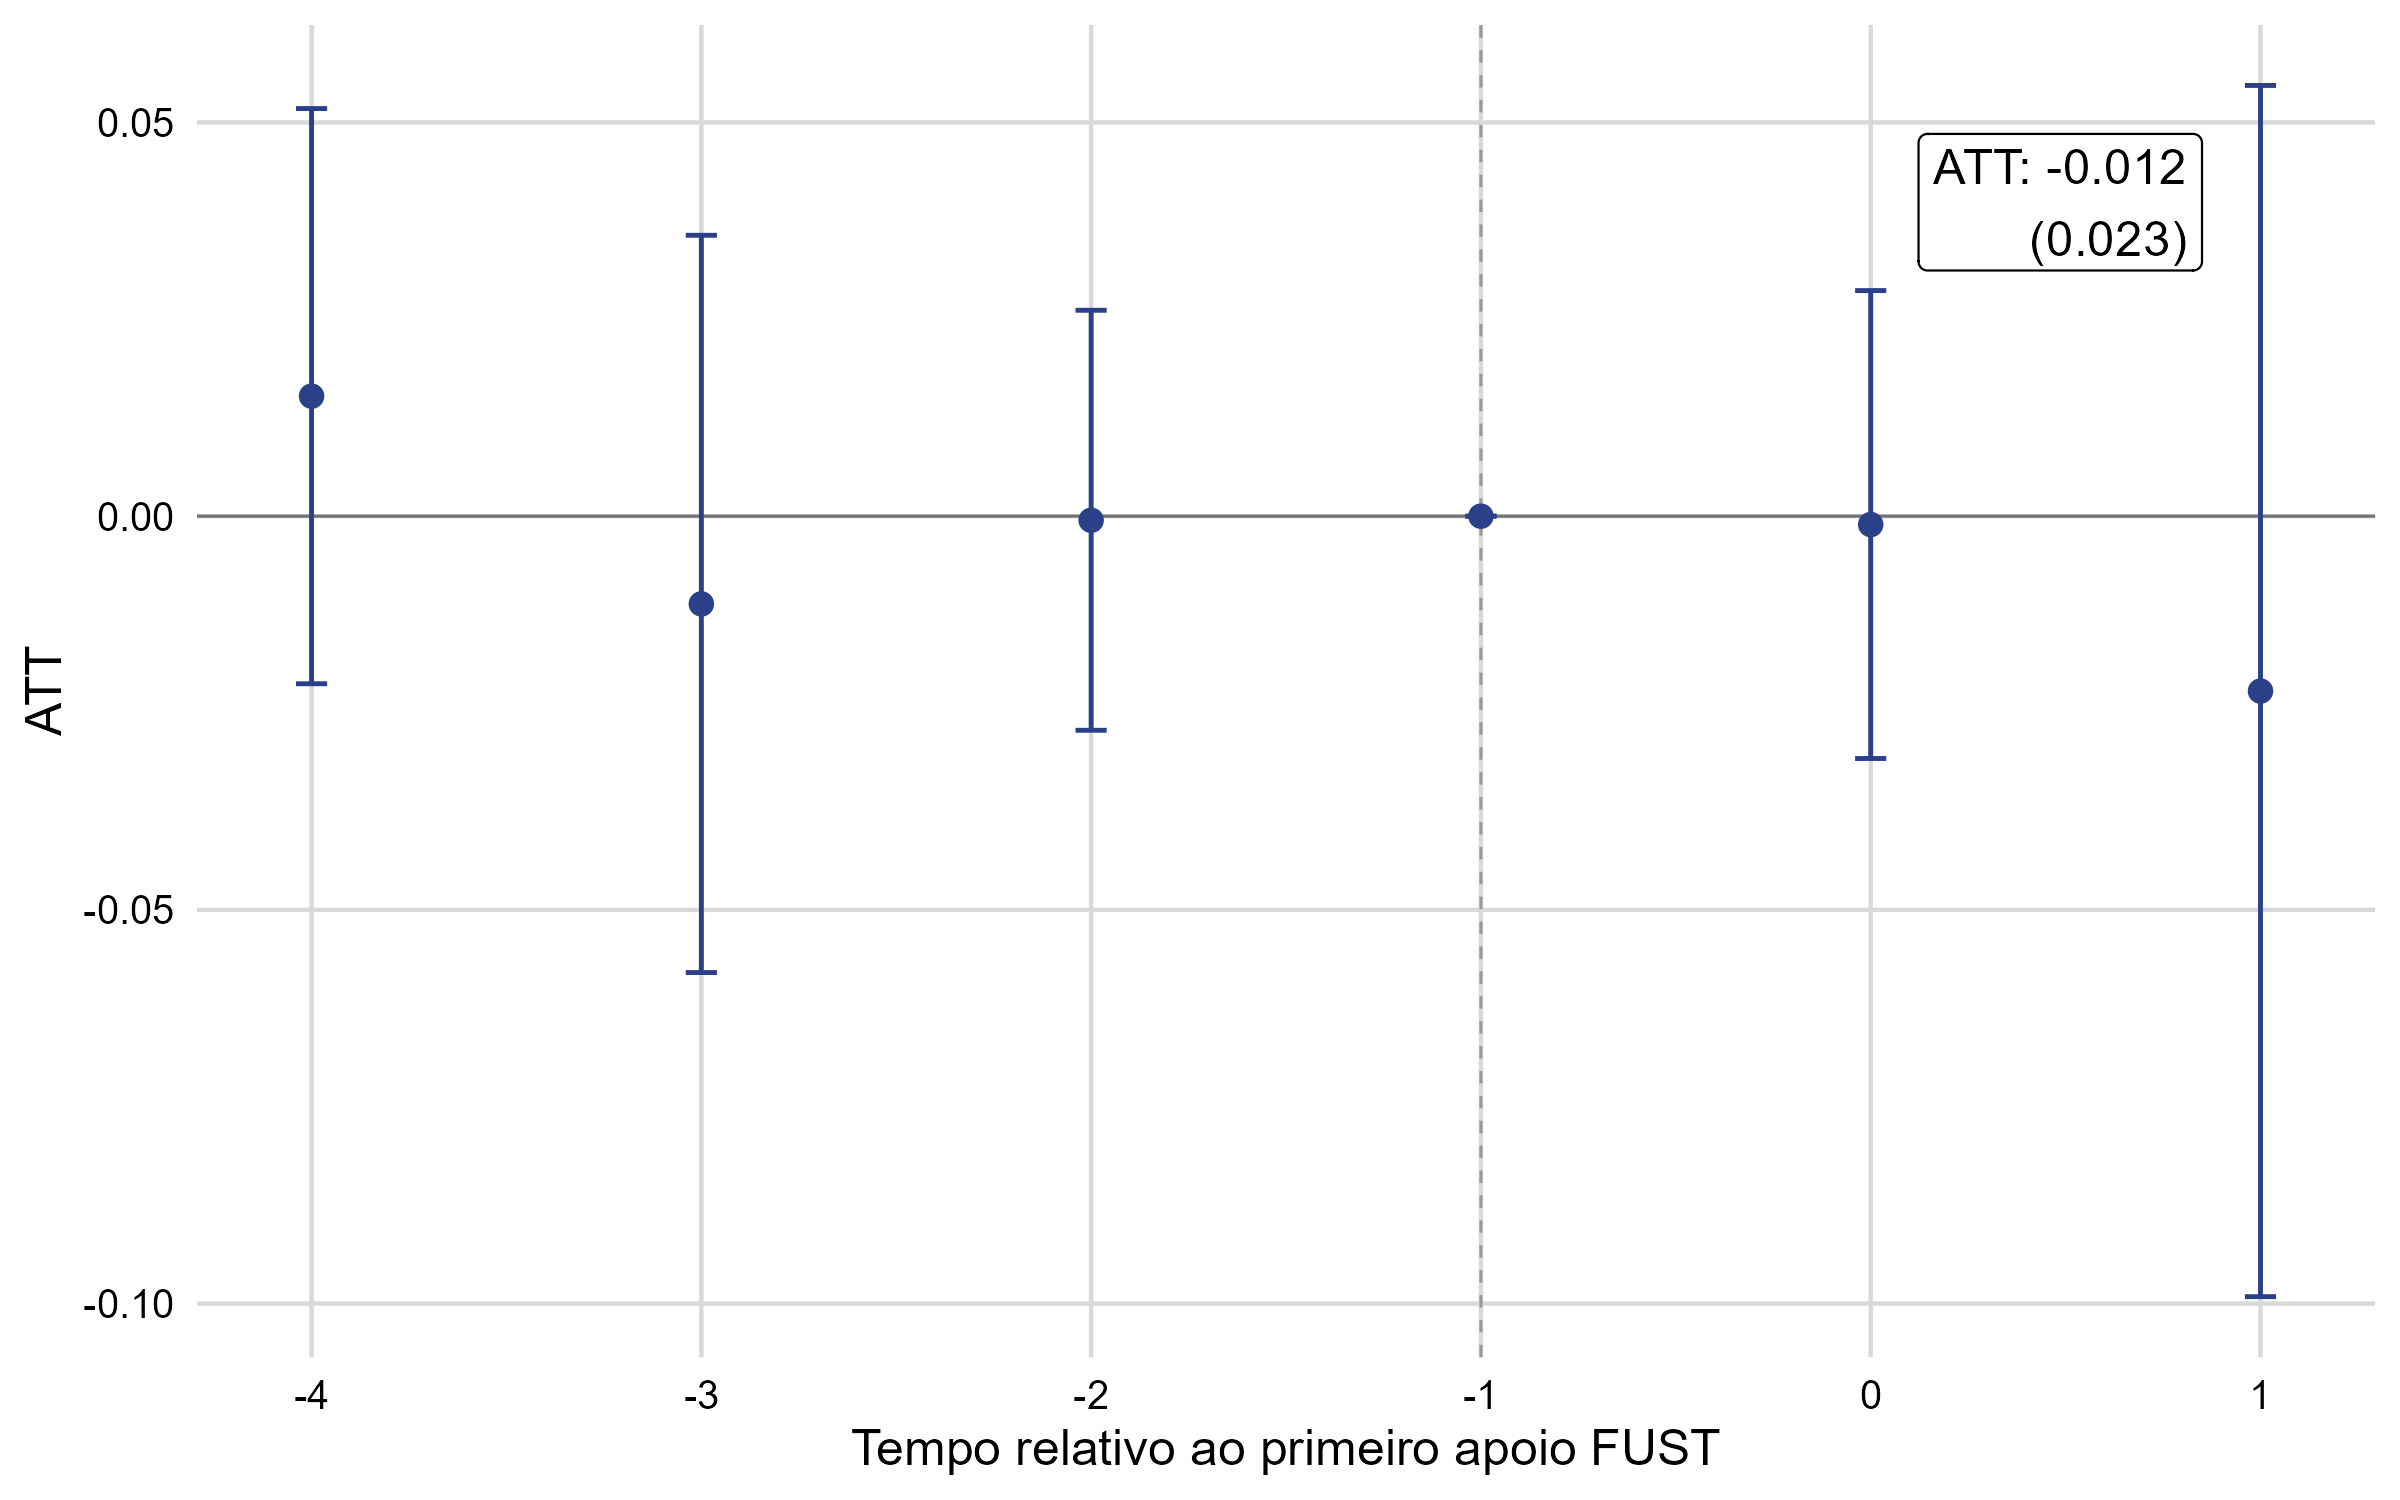
\includegraphics[width=0.96\textwidth]{Event study - CS - Log-salario-medio.png}
\caption{Estudo de evento: salário médio}
\label{fig:es_salario}
\figurenote{Estimador de Callaway--Sant'Anna. O período $e=-1$ é a referência. Pontos são ATTs por
tempo relativo e barras representam intervalos pontuais de 95\%.}
\end{figure}

\clearpage
\subsection{Heterogeneidade}

As heterogeneidades são estimadas refazendo o pareamento para cada subgrupo e coorte. O algoritmo
seleciona um vizinho por distância de Mahalanobis, com pareamento exato pela divisão da CNAE,
razão 1:1 e sem reposição; quando a distância de Mahalanobis não pode ser calculada, utiliza-se
propensity score mantendo a razão 1:1, a restrição setorial e a ausência de reposição. Assim, cada
amostra efetivamente estimada contém o mesmo número de tratadas e controles.

Uma auditoria da base final verificou 1.650 pares: todos contêm exatamente uma empresa tratada e
uma empresa controle, não há pares inválidos e nenhum controle é reutilizado dentro do mesmo
subgrupo. Quando não existe controle compatível em um estrato exato, a tratada correspondente
fica fora daquela estimação. Portanto, os avisos de escassez de controles reduzem o suporte do
subgrupo, mas não rompem a razão 1:1. Como cada heterogeneidade é uma análise independente, um
mesmo controle pode aparecer em recortes diferentes.

Os cortes também são definidos de forma explícita. A idade da firma é separada pela mediana entre
as tratadas: até 14 anos e maior que 14 anos. A qualificação corresponde à proporção de
trabalhadores com ensino superior no ano anterior ao tratamento; baixa qualificação significa até
23,75% e alta qualificação, mais de 23,75%. O porte segue a classificação do BNDES, reunindo
micro e pequena e mantendo média e grande separadas. Filiais distinguem uma unidade de mais de
uma unidade, com a informação do ano anterior ao apoio. Subcréditos distinguem empresas com um
subcrédito daquelas com mais de um, conforme a base operacional do FUST.

As figuras apresentam efeitos separados, mas não testes formais da diferença entre subgrupos.
Além disso, alguns recortes têm poucas tratadas, sobretudo porte grande (7), apoio direto (17),
região Sul (34) e mais de um subcrédito (47), gerando intervalos amplos.

\begin{table}[H]
\centering
\caption{Composição efetiva das amostras de heterogeneidade}
\label{tab:hetero_samples}
\footnotesize
\setlength{\tabcolsep}{7pt}
\begin{tabular}{llrr}
\toprule
Dimensão & Grupo & Tratadas & Controles \\
\midrule
Modalidade & Direta & 17 & 17 \\
Modalidade & Indireta & 207 & 207 \\
Porte BNDES & Micro e pequena & 79 & 79 \\
Porte BNDES & Média & 138 & 138 \\
Porte BNDES & Grande & 7 & 7 \\
Setor & Telecom por fio & 144 & 144 \\
Setor & Outras telecom & 66 & 66 \\
Região & Sul & 34 & 34 \\
Região & Sudeste & 78 & 78 \\
Região & Outras regiões & 54 & 54 \\
Idade da firma & Até 14 anos & 117 & 117 \\
Idade da firma & Maior que 14 anos & 70 & 70 \\
Qualificação & Até 23,75\% com ensino superior & 112 & 112 \\
Qualificação & Mais de 23,75\% com ensino superior & 79 & 79 \\
Filiais & Uma unidade & 159 & 159 \\
Filiais & Mais de uma unidade & 65 & 65 \\
Subcréditos & Um subcrédito & 177 & 177 \\
Subcréditos & Mais de um subcrédito & 47 & 47 \\
\bottomrule
\end{tabular}
\figurenote{Cada linha corresponde a uma estimação independente. As contagens são de CNPJ-raiz
únicos na amostra pareada final. A igualdade entre as duas últimas colunas confirma a razão 1:1.}
\end{table}

\subsubsection{Emprego}

Os efeitos sobre emprego são positivos em quase todos os grupos. Destacam-se outras atividades de
telecomunicações (aprox. \pct{48,5}), outras regiões fora do Sul e Sudeste (\pct{47,1}), empresas
micro ou pequenas pela classificação BNDES (\pct{45,1}) e empresas com alta qualificação prévia
(\pct{47,2}). O efeito é praticamente igual entre firmas com até 14 anos (\pct{32,8}) e com mais
de 14 anos (\pct{32,0}), e também próximo entre um subcrédito (\pct{27,5}) e mais de um
(\pct{31,1}). Empresas com uma unidade apresentam estimativa de \pct{31,8}, ante \pct{24,4}
naquelas com mais de uma unidade. A principal exceção é a região Sul, com estimativa de
$-4,5\%$ e intervalo que inclui zero. Esses contrastes são sugestivos, mas não constituem testes
formais de diferença entre grupos.

\begin{figure}[p]
\centering
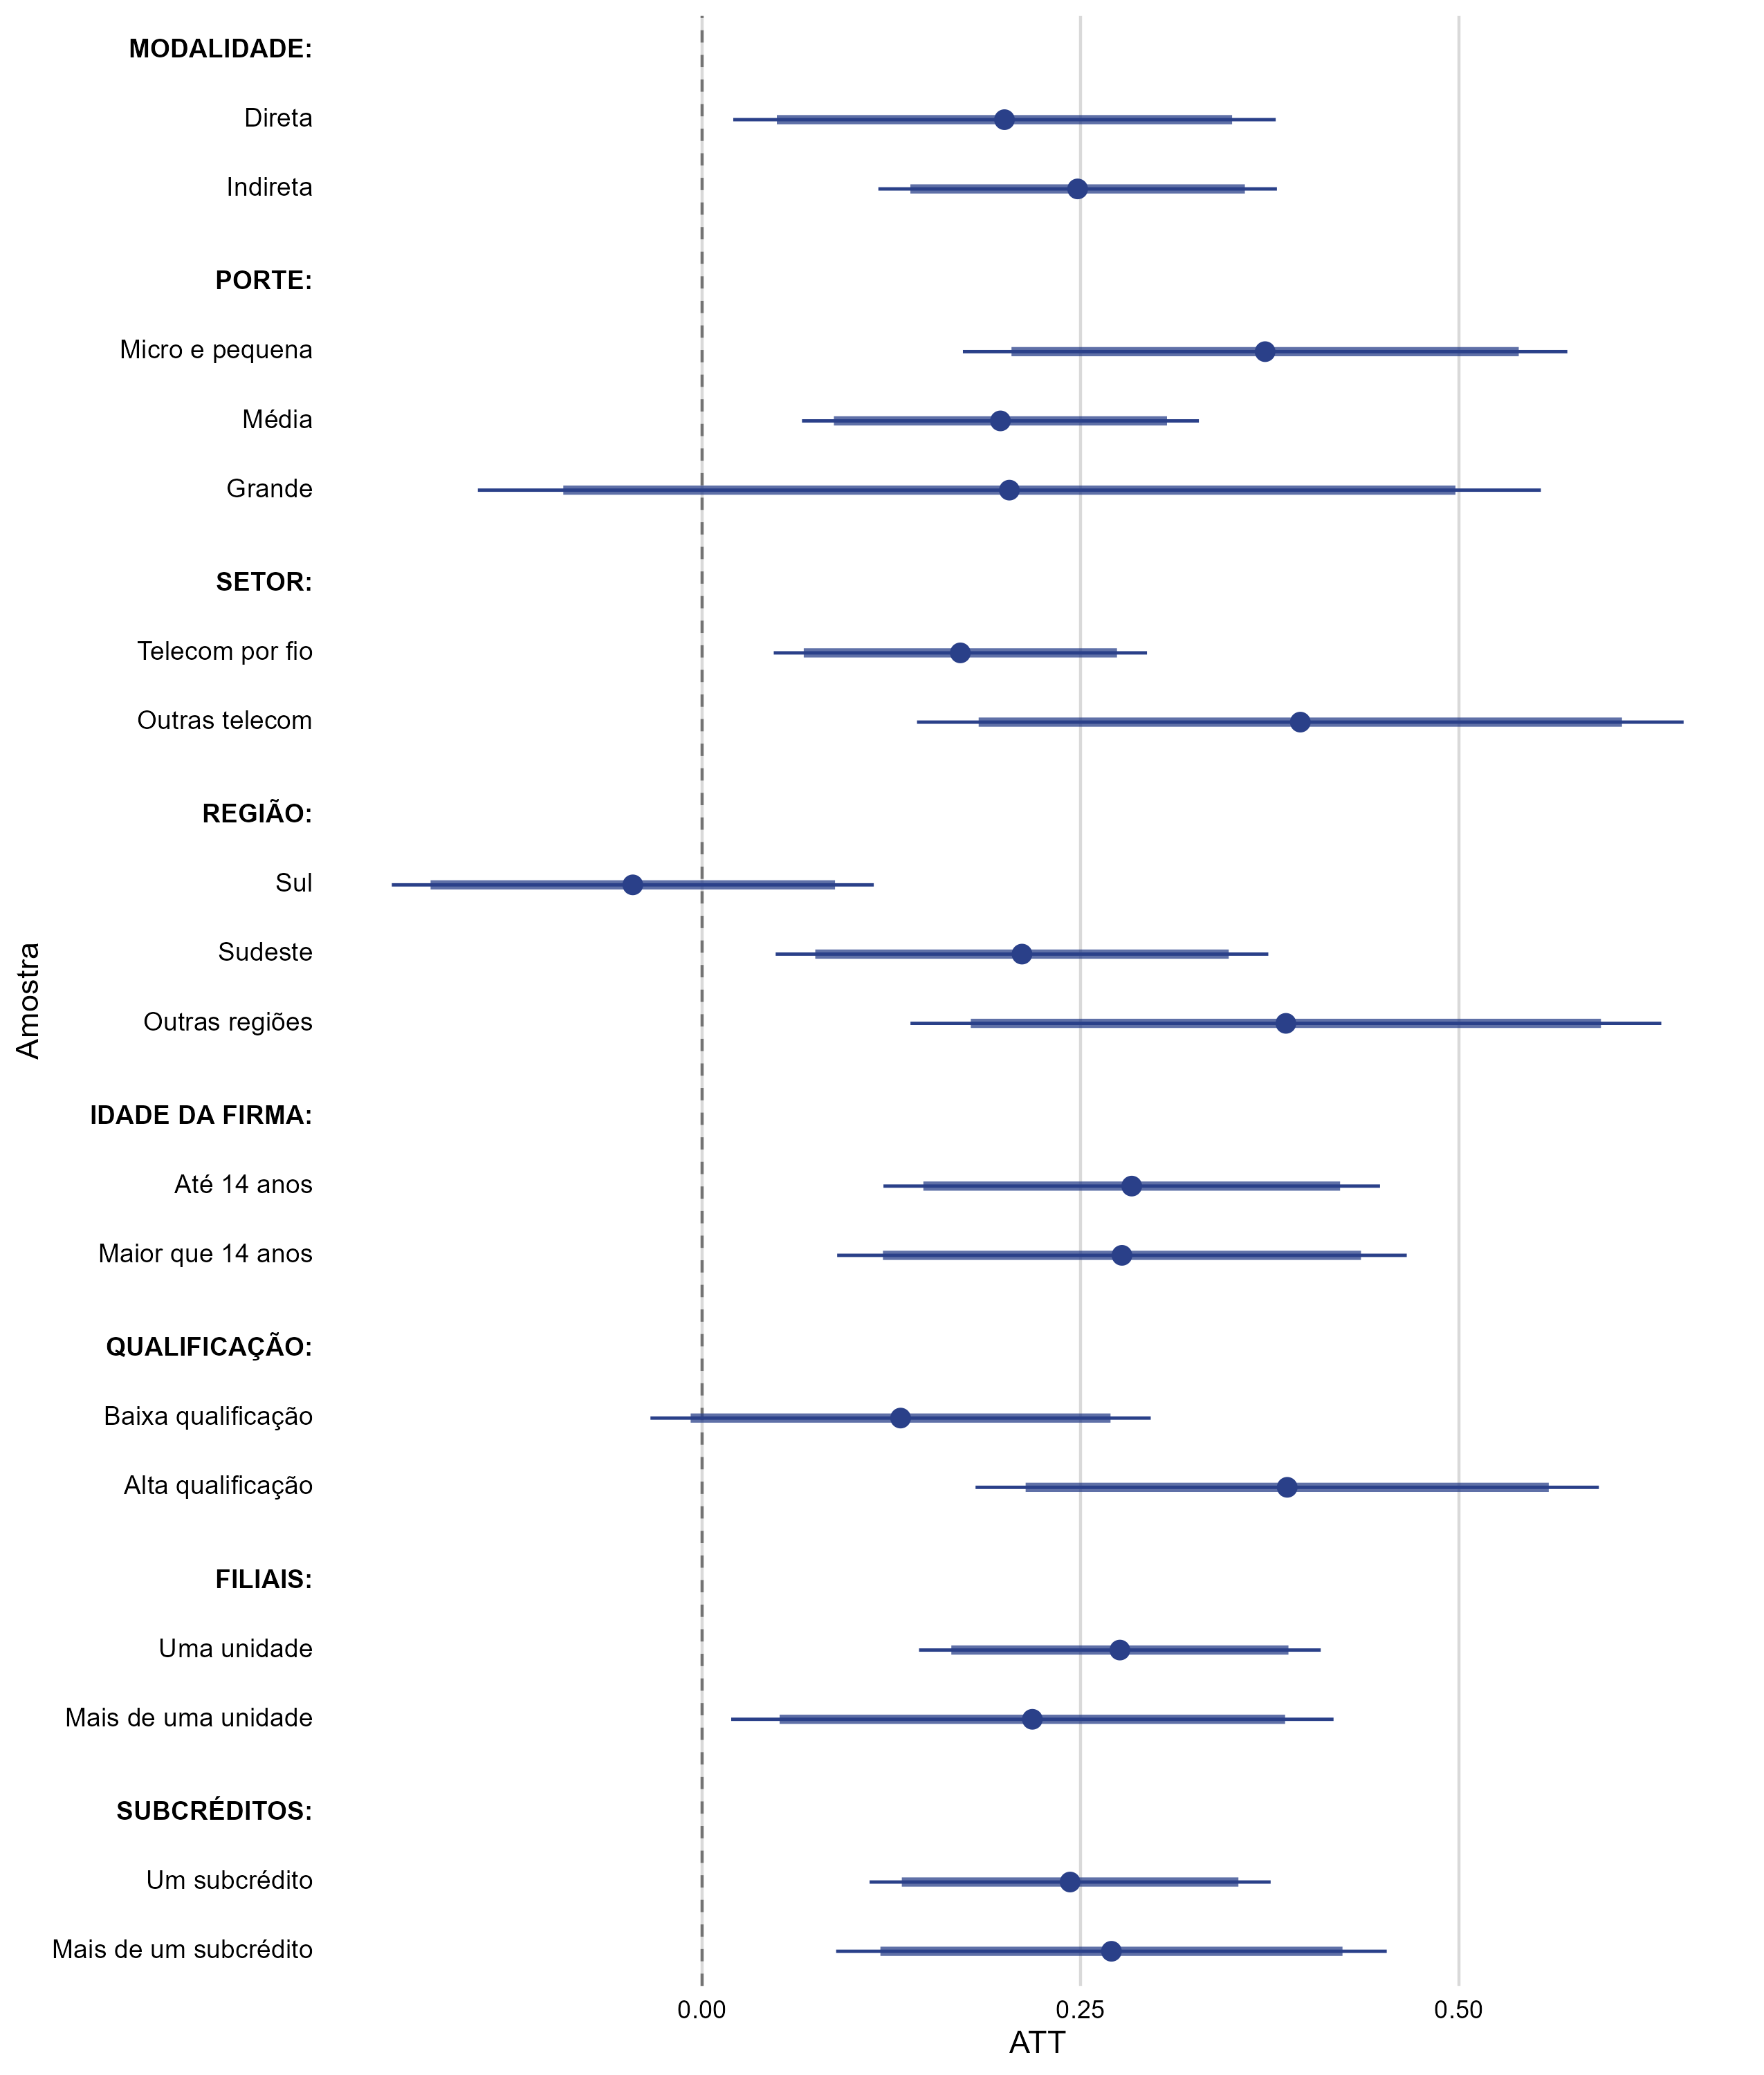
\includegraphics[width=\textwidth,height=0.82\textheight,keepaspectratio]{Heterogeneidades - Log-emprego.png}
\caption{Heterogeneidade dos efeitos sobre emprego}
\label{fig:het_emprego}
\figurenote{Cada ponto é o ATT médio de uma amostra pareada dentro do subgrupo. As barras grossas
e finas representam intervalos de 90\% e 95\%, respectivamente.}
\end{figure}

\subsubsection{Massa salarial}

As estimativas de massa salarial são, em geral, positivas, porém menos precisas. Há efeitos
estatisticamente significativos para apoio indireto (aprox. \pct{56,7}), porte médio
(\pct{71,0}), outras atividades de telecomunicações (\pct{87,0}), os dois grupos de idade,
empresas de alta qualificação (\pct{144,2}), unidades únicas (\pct{42,2}) e empresas com um
subcrédito (\pct{50,0}). Micro e pequenas apresentam estimativa de \pct{45,5}, enquanto grandes
apresentam \pct{26,1}; ambos os intervalos incluem zero, e o grupo de grandes contém apenas sete
pares. Firmas com mais de uma unidade e com mais de um subcrédito também têm estimativas positivas,
mas intervalos mais largos. As magnitudes elevadas em alguns recortes não devem ser lidas como um
ranking preciso.

\begin{figure}[p]
\centering
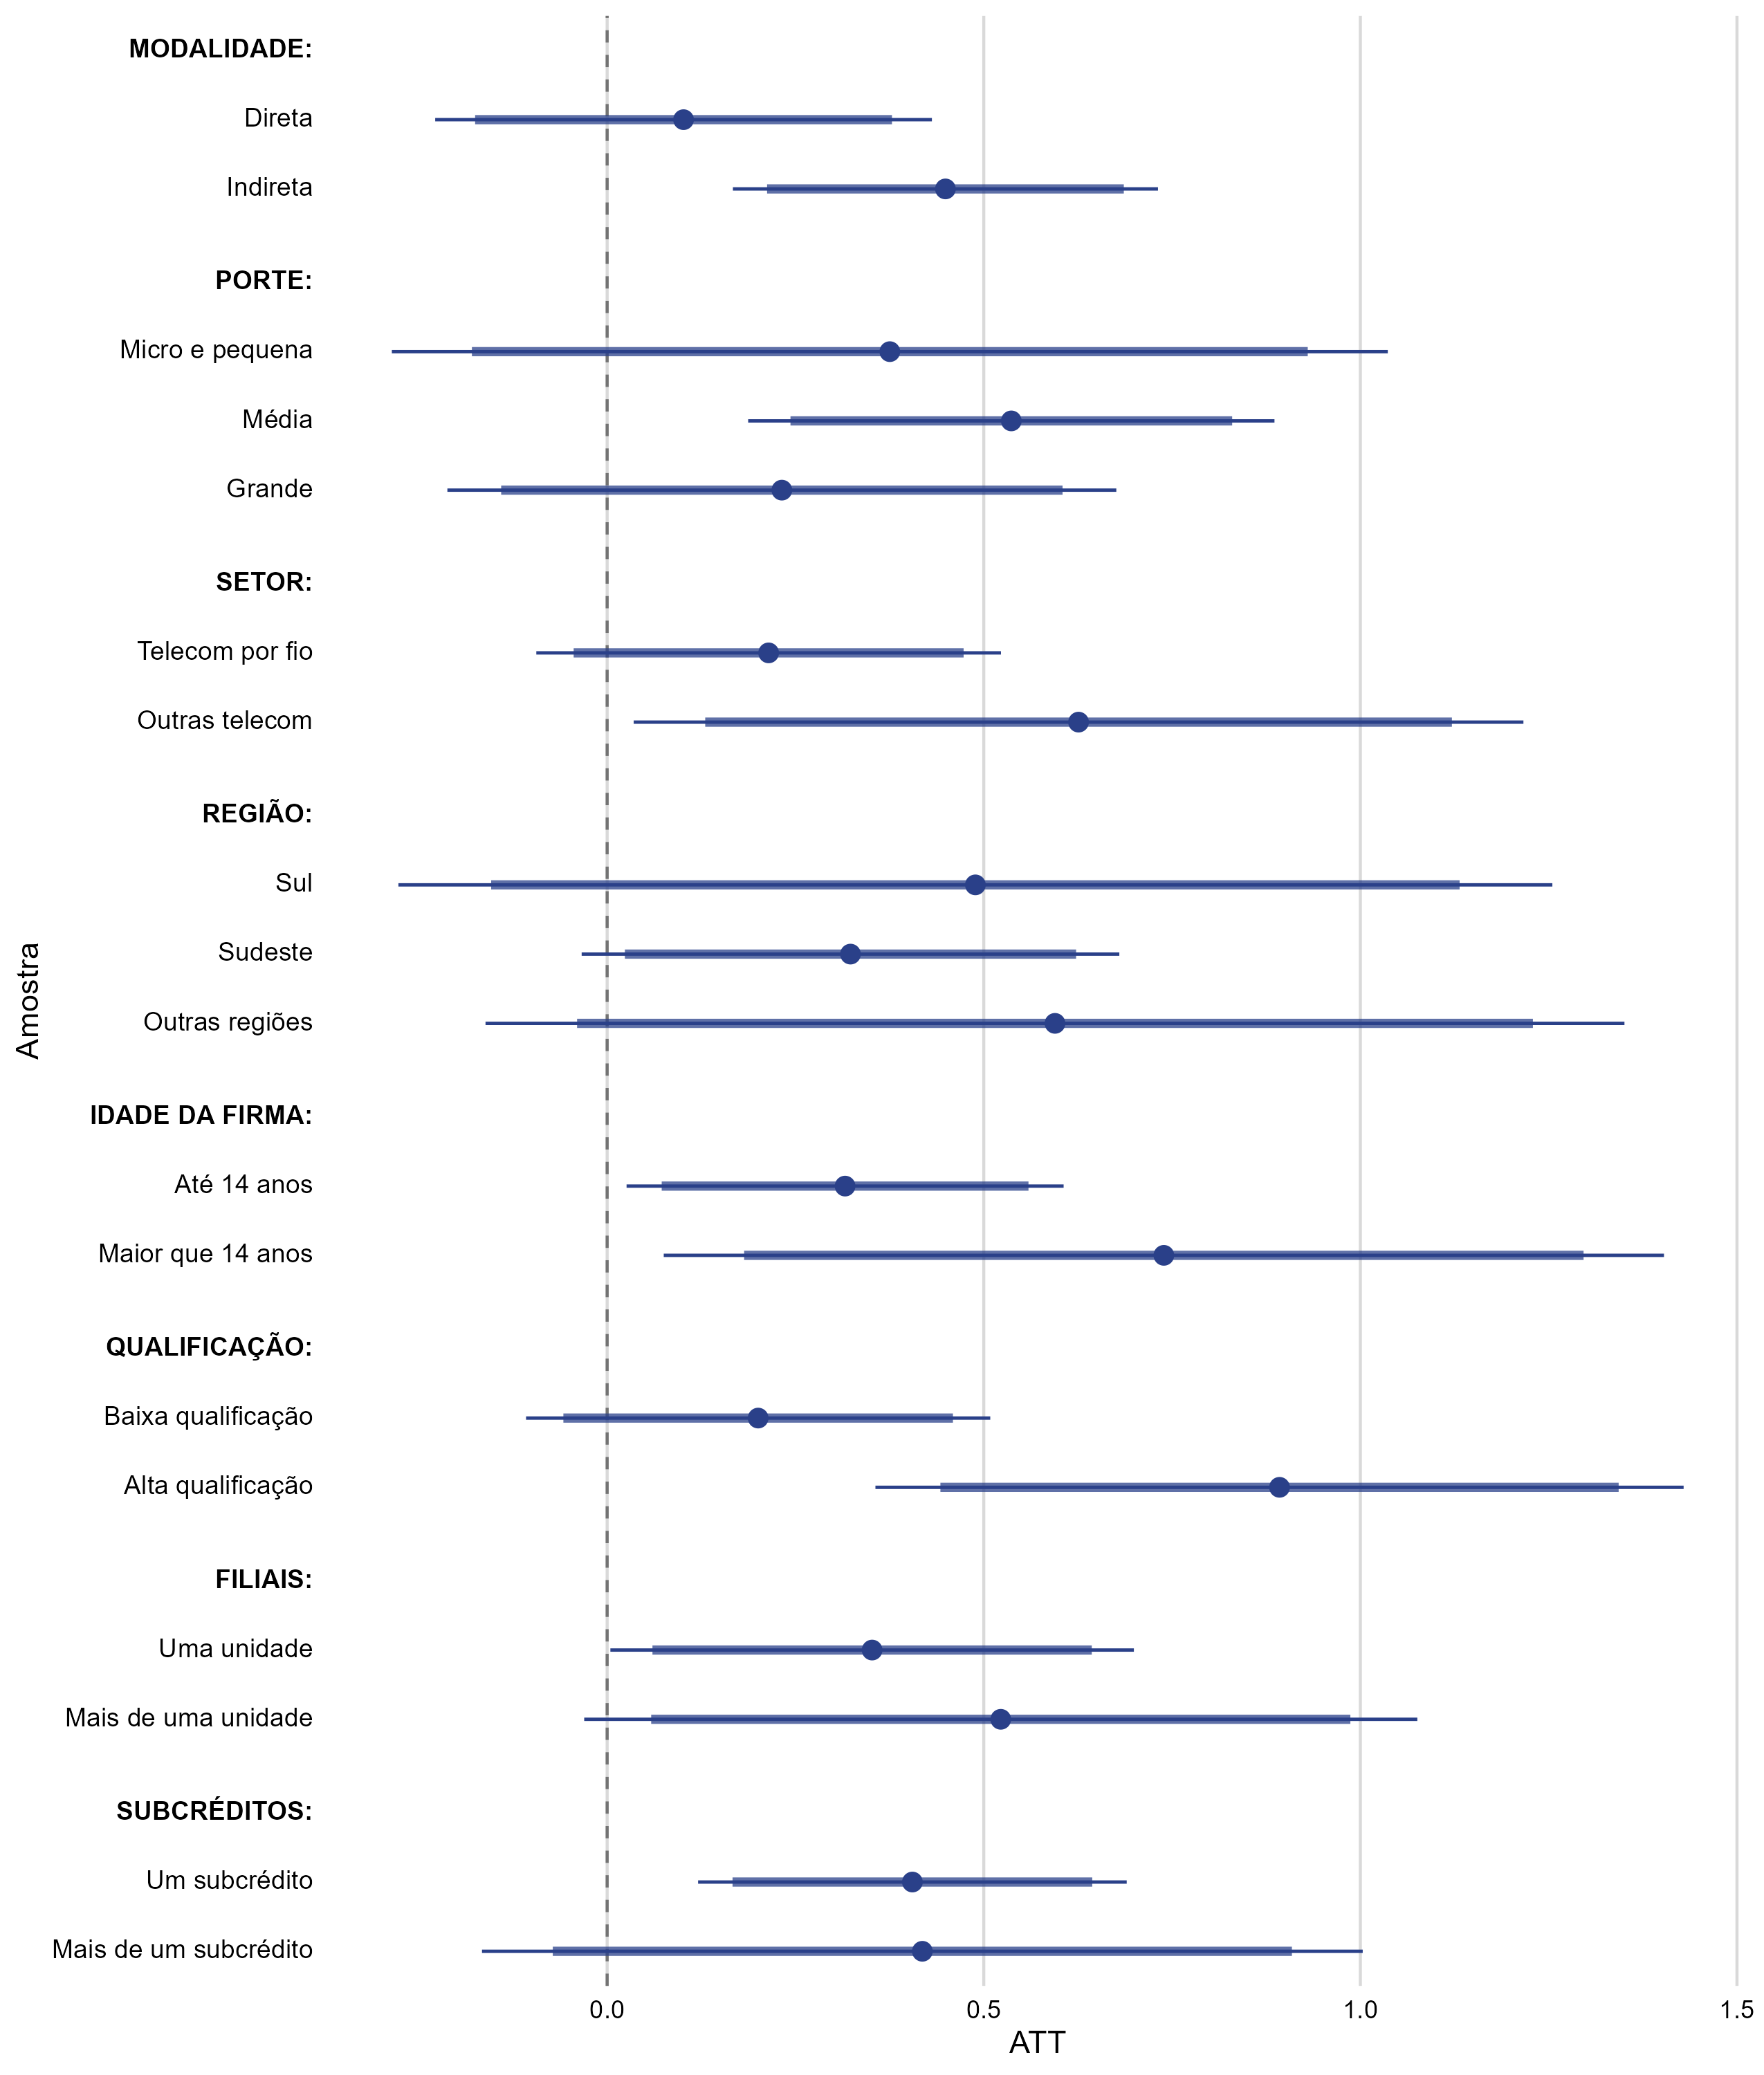
\includegraphics[width=\textwidth,height=0.82\textheight,keepaspectratio]{Heterogeneidades - Log-massa-salarial.png}
\caption{Heterogeneidade dos efeitos sobre massa salarial}
\label{fig:het_massa}
\figurenote{Cada ponto é o ATT médio de uma amostra pareada dentro do subgrupo. As barras grossas
e finas representam intervalos de 90\% e 95\%, respectivamente.}
\end{figure}

\subsubsection{Salário médio}

Para quase todos os recortes, o efeito sobre salário médio permanece próximo de zero e impreciso.
Duas exceções se destacam. Na região Sul, a estimativa é 0,053 (aprox. \pct{5,5}) e o limite
inferior do intervalo de 95\% fica muito próximo de zero. Para empresas de grande porte, a
estimativa é $-0,063$ (aprox. $-6,1\%$) e o intervalo de 95\% não inclui zero; esse resultado,
contudo, se apoia em apenas sete pares. Os dois achados devem ser vistos como hipóteses para
investigação adicional, sobretudo porque não houve correção para múltiplas comparações.

\begin{figure}[p]
\centering
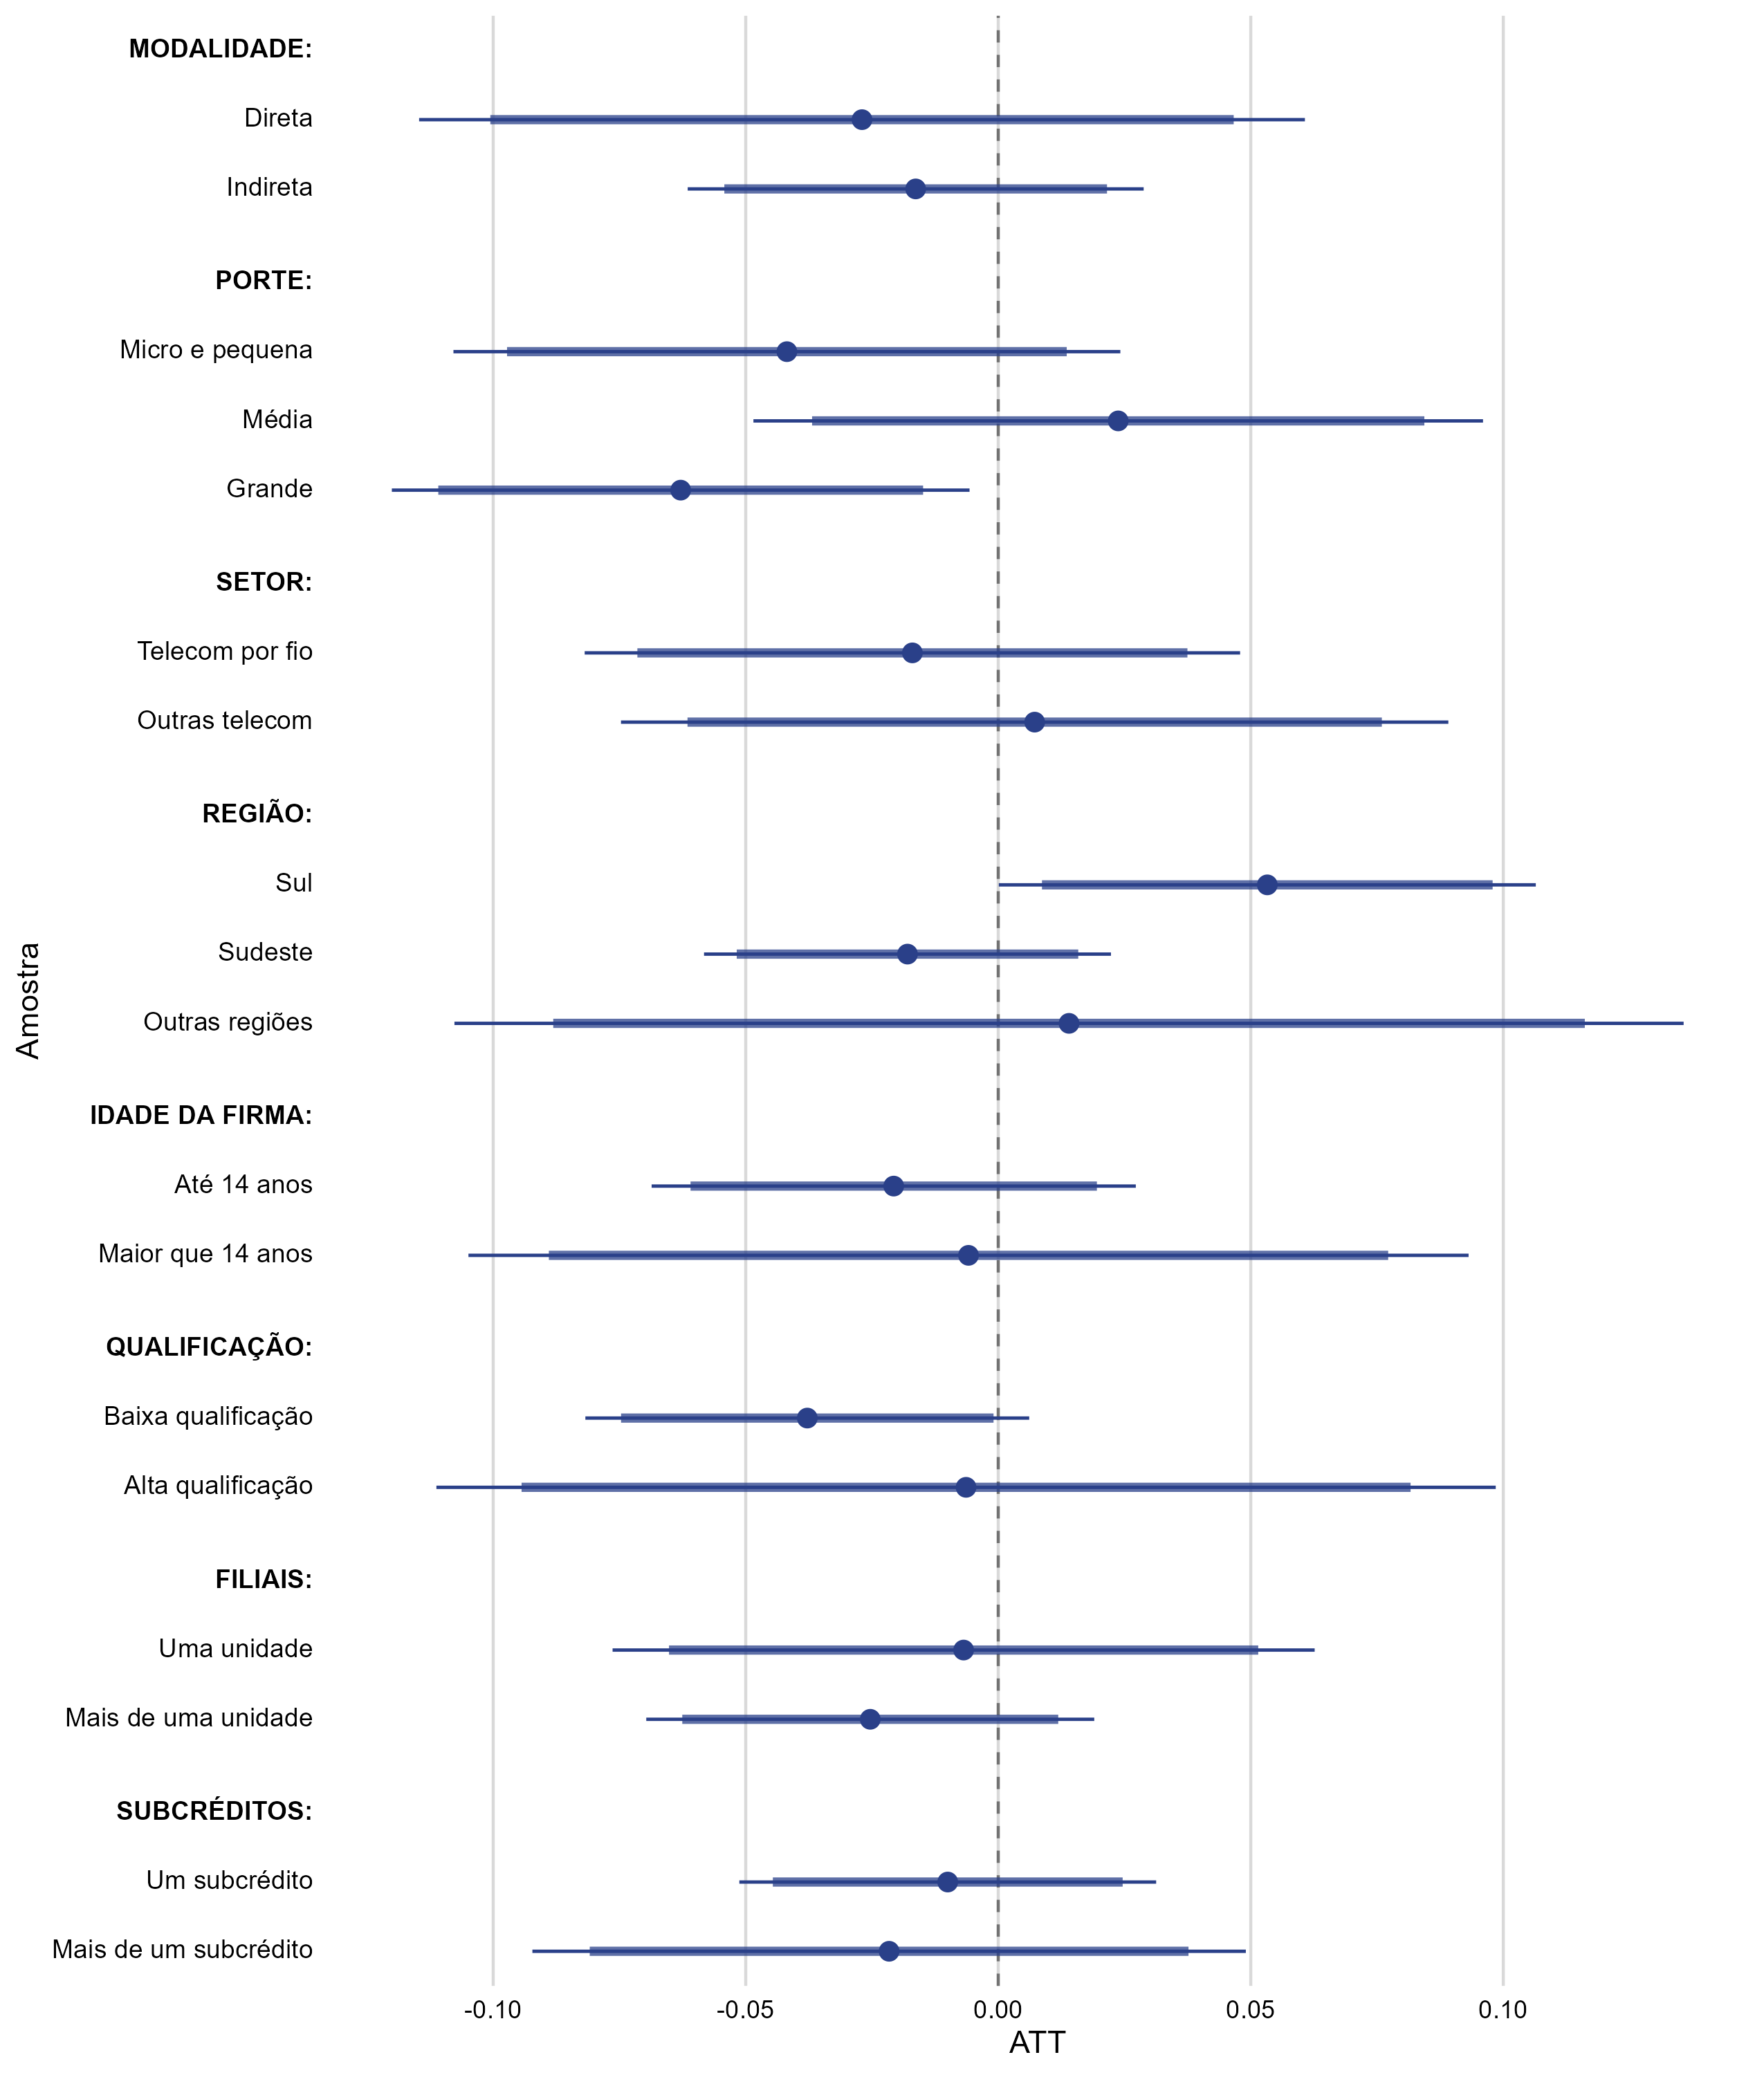
\includegraphics[width=\textwidth,height=0.82\textheight,keepaspectratio]{Heterogeneidades - Log-salario-medio.png}
\caption{Heterogeneidade dos efeitos sobre salário médio}
\label{fig:het_salario}
\figurenote{Cada ponto é o ATT médio de uma amostra pareada dentro do subgrupo. As barras grossas
e finas representam intervalos de 90\% e 95\%, respectivamente.}
\end{figure}

\clearpage
\subsection{Interpretação conjunta}

O conjunto dos resultados é consistente com expansão de curto prazo das empresas apoiadas. O
emprego cresce no ano do apoio e mais ainda no ano seguinte; a massa salarial apresenta dinâmica
semelhante; e o salário médio não mostra aumento sistemático. A evidência é mais estável para
emprego, inclusive nas análises de sensibilidade. Para massa salarial, a direção positiva é
recorrente, mas a precisão é menor. Para salário médio, especificações alternativas chegam a
indicar queda no ano seguinte, de modo que a conclusão deve permanecer agnóstica quanto a um
efeito salarial positivo.

As limitações centrais são a janela pós-tratamento curta, o balanceamento incompleto em duas
covariadas, a rejeição dos testes conjuntos de pré-tendências para emprego e salário médio e a
pequena dimensão de alguns subgrupos. Esses pontos não eliminam os resultados, mas condicionam a
linguagem causal: a expansão do emprego é o achado mais robusto; as demais conclusões exigem maior
prudência.

% -----------------------------------------------------------------------------
\clearpage
\appendix
\renewcommand{\thefigure}{A\arabic{figure}}
\setcounter{figure}{0}
\renewcommand{\thetable}{A\arabic{table}}
\setcounter{table}{0}

\section{Apêndice: testes de robustez}

Este apêndice reúne todas as doze figuras de robustez disponíveis em \texttt{analysis}. Elas
avaliam inferência e controles alternativos, regras de pareamento, estimadores alternativos e
sensibilidade a violações de tendências paralelas.

\subsection{Inferência, controles, dependência espacial e placebo}

Para emprego, o efeito permanece positivo e significativo com agrupamento por município ou UF,
erros de Conley com raio de 200 km e controles pré-FUST interagidos com ano. As estimativas dessas
especificações TWFE ficam entre 0,303 e 0,318. O placebo que antecipa artificialmente o tratamento
em dois anos é pequeno e não significativo (0,029; erro-padrão 0,056).

Para massa salarial, as alternativas produzem estimativas entre 0,443 e 0,504, todas positivas e
significativas; o placebo é 0,210 e não significativo. Para salário médio, a conclusão é menos
uniforme: a estimativa principal é nula, enquanto a especificação TWFE agrupada por município
indica $-0,063$ e significância a 5\%; com agrupamento por UF, Conley e controles, a evidência é
limítrofe ou não significativa a 5\%. O placebo permanece nulo.

\begin{figure}[p]
\centering
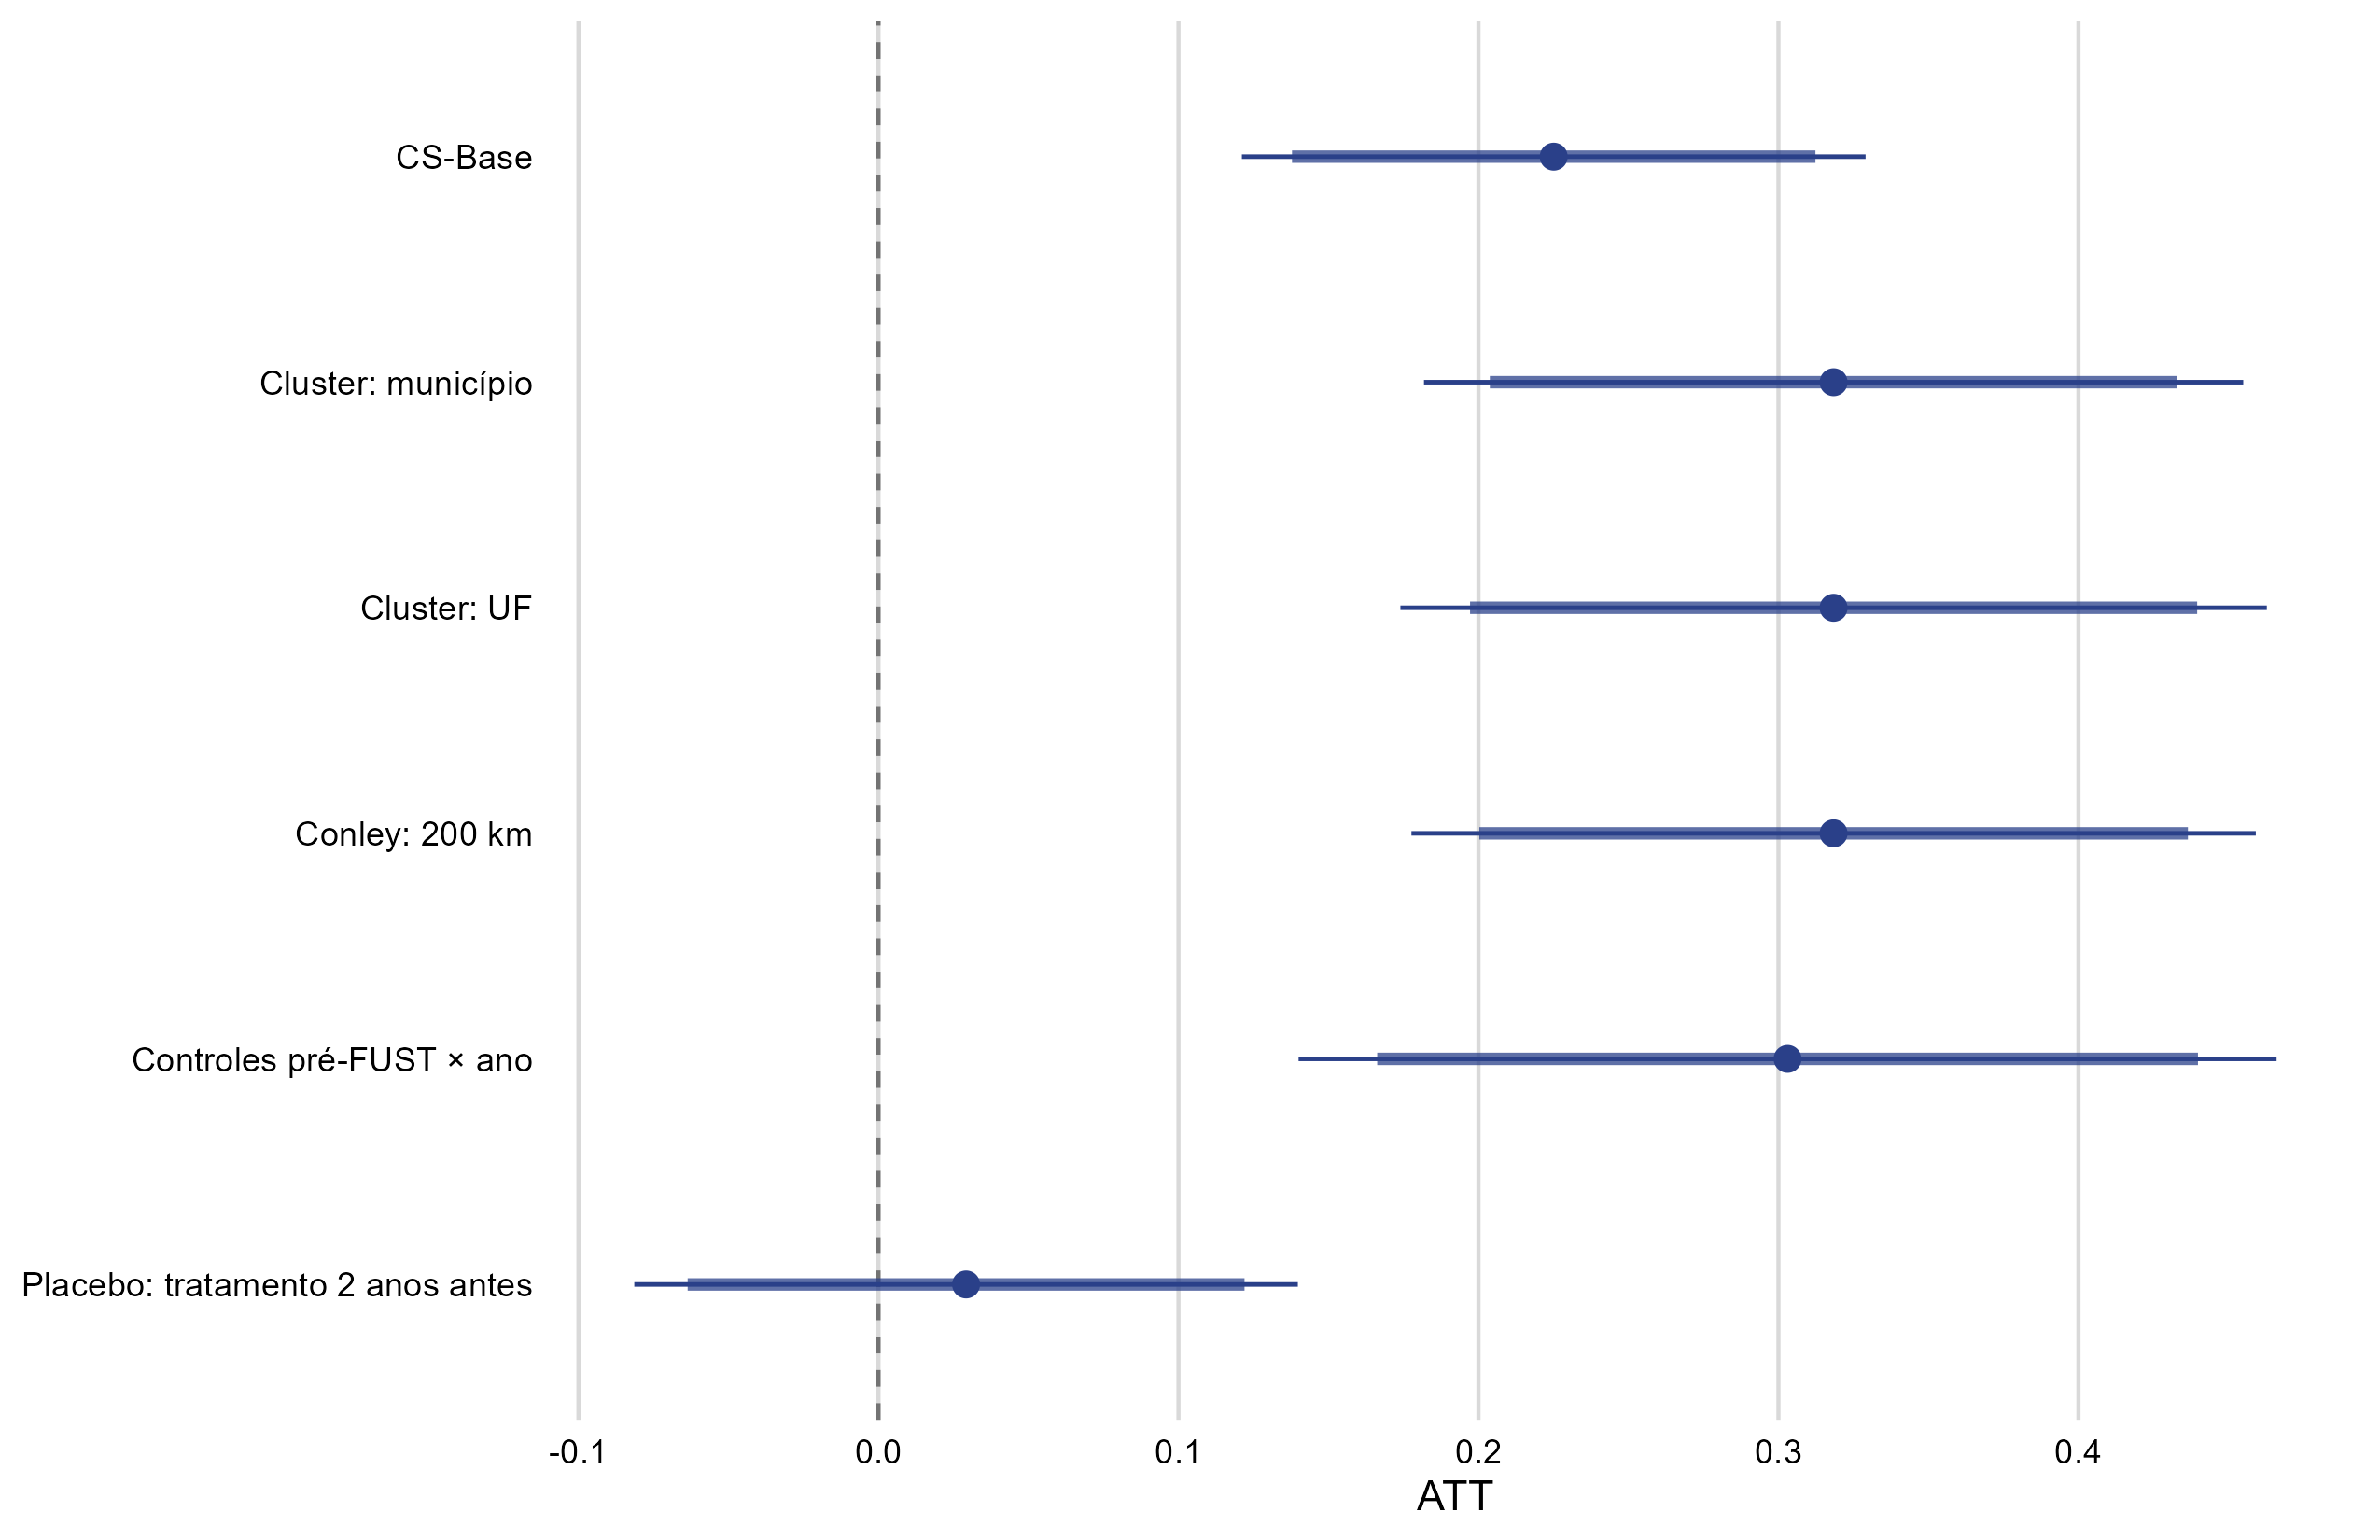
\includegraphics[width=0.96\textwidth]{Robustez - Log-emprego.png}
\caption{Robustez geral: emprego}
\label{fig:rob_geral_emp}
\figurenote{Barras grossas e finas: intervalos de 90\% e 95\%. A linha CS-Base usa o estimador
principal; as linhas de agrupamento, Conley e controles usam TWFE.}
\end{figure}

\begin{figure}[p]
\centering
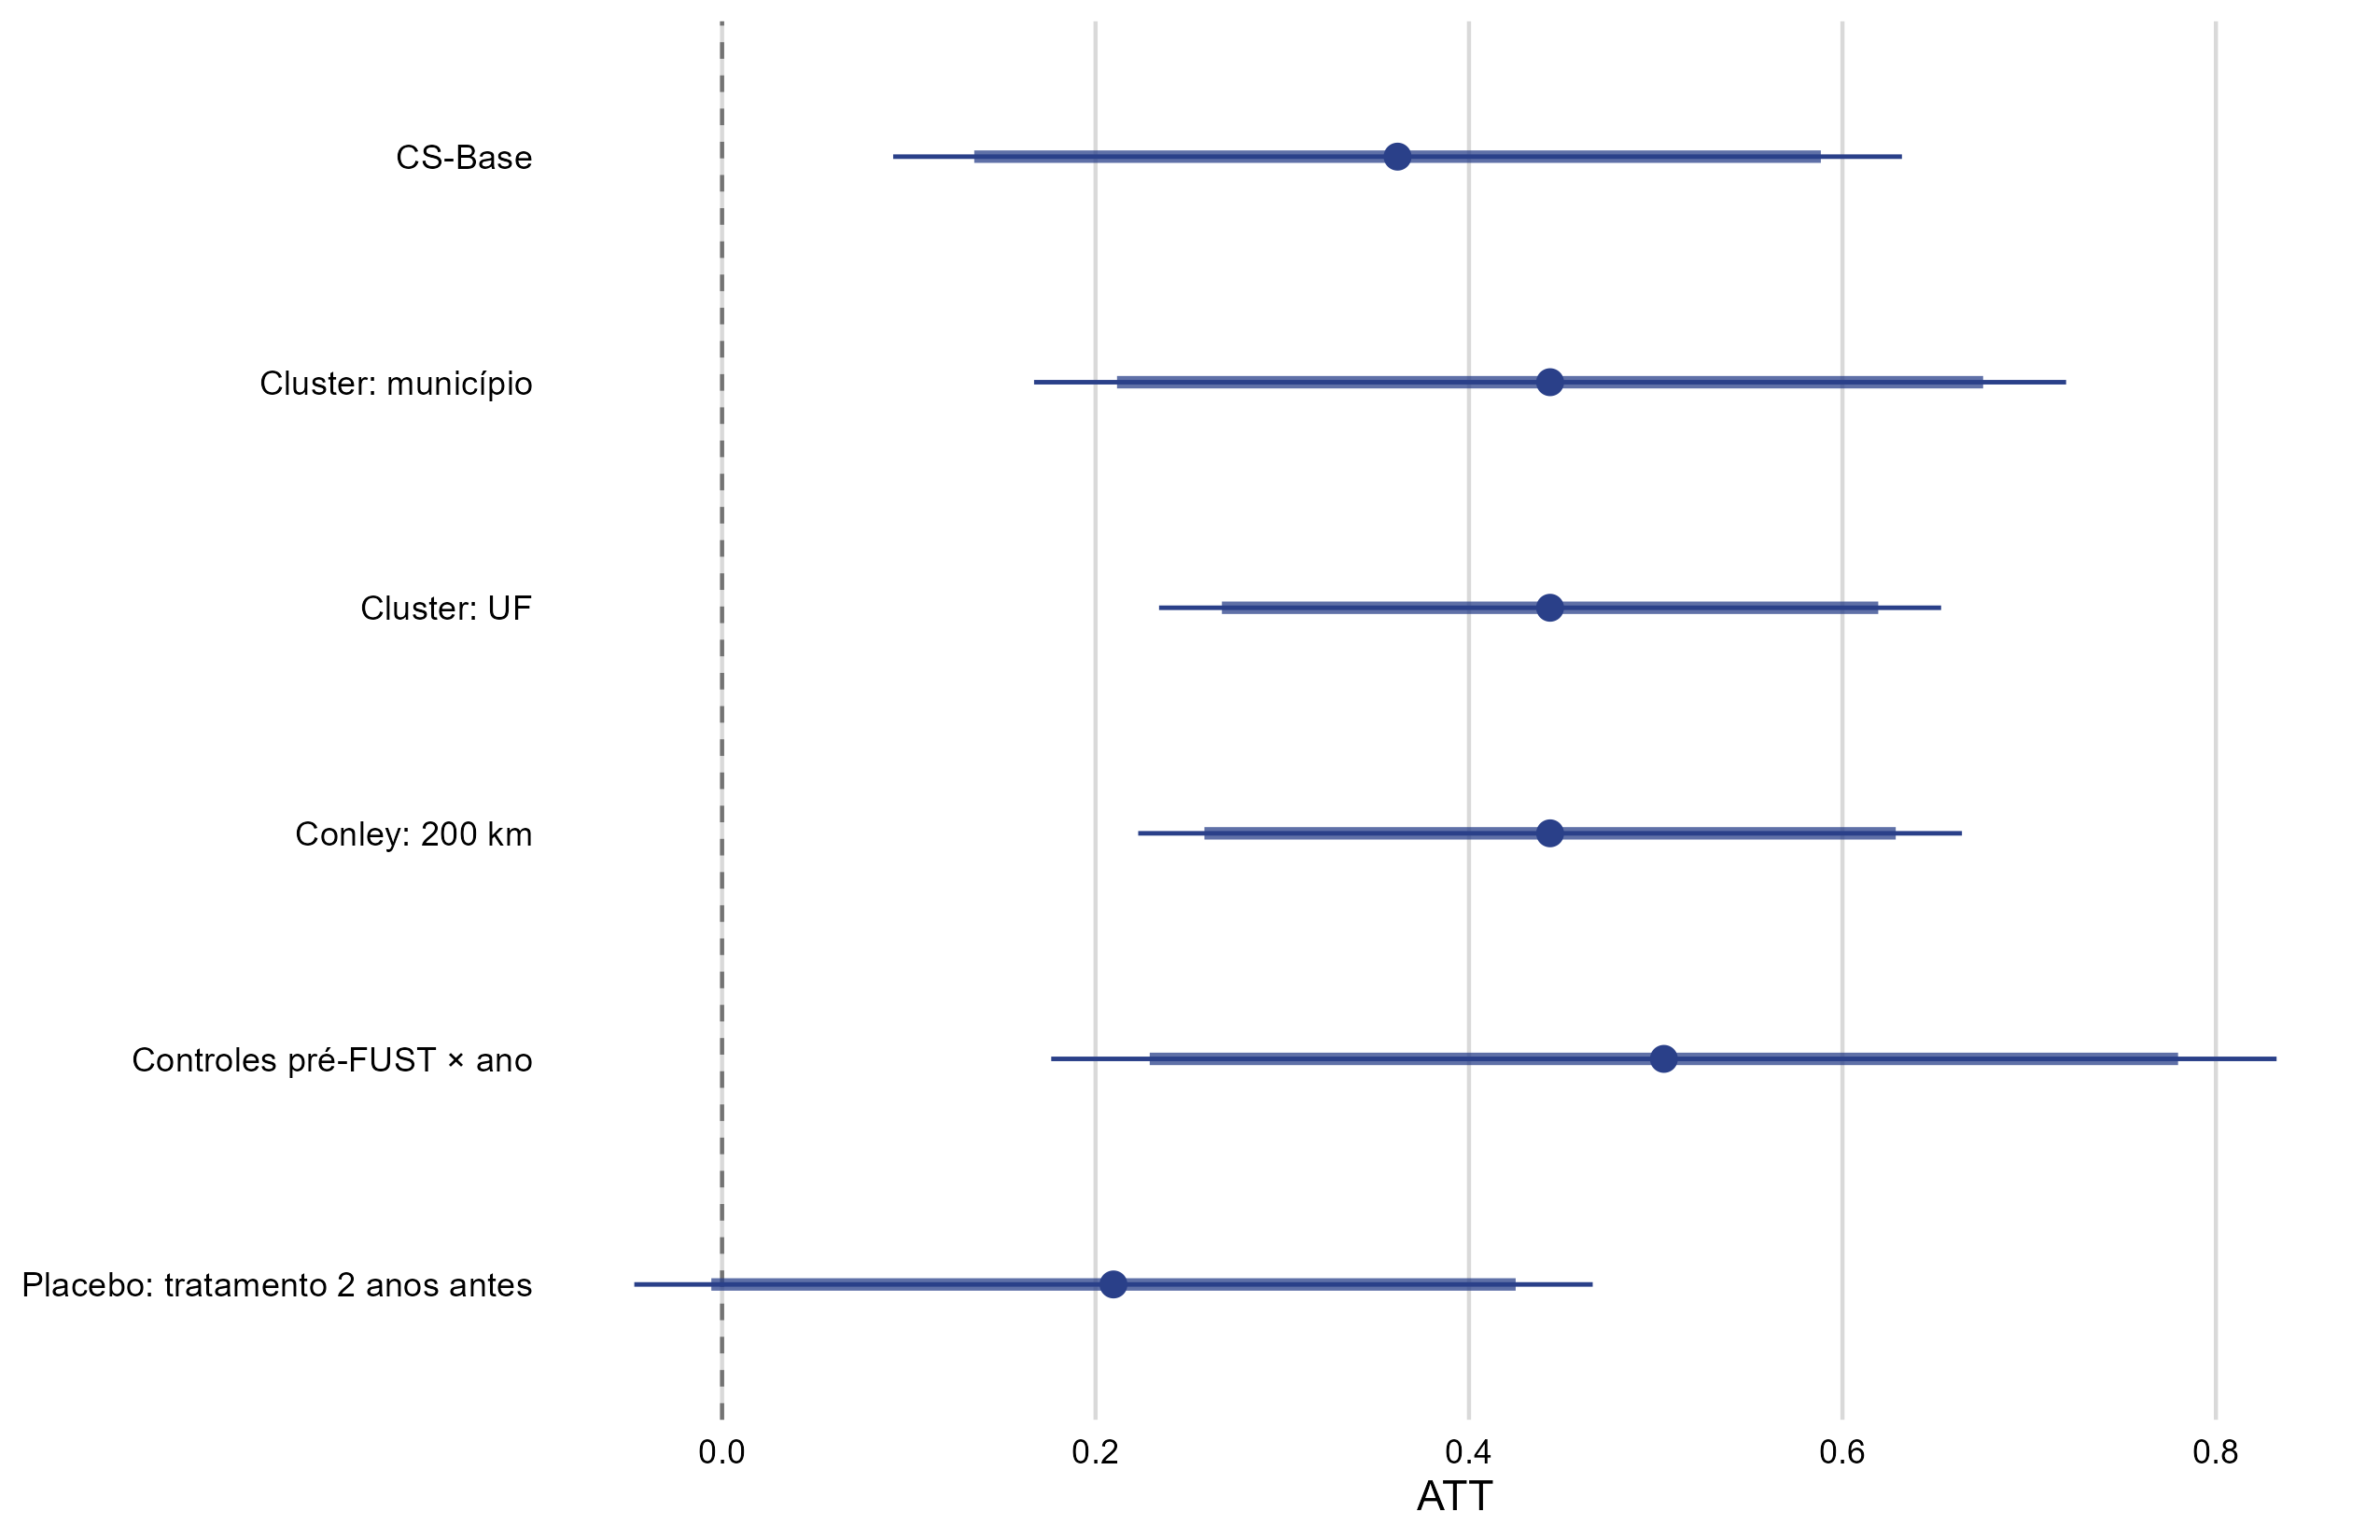
\includegraphics[width=0.96\textwidth]{Robustez - Log-massa-salarial.png}
\caption{Robustez geral: massa salarial}
\label{fig:rob_geral_massa}
\figurenote{Barras grossas e finas: intervalos de 90\% e 95\%. A linha CS-Base usa o estimador
principal; as linhas de agrupamento, Conley e controles usam TWFE.}
\end{figure}

\begin{figure}[p]
\centering
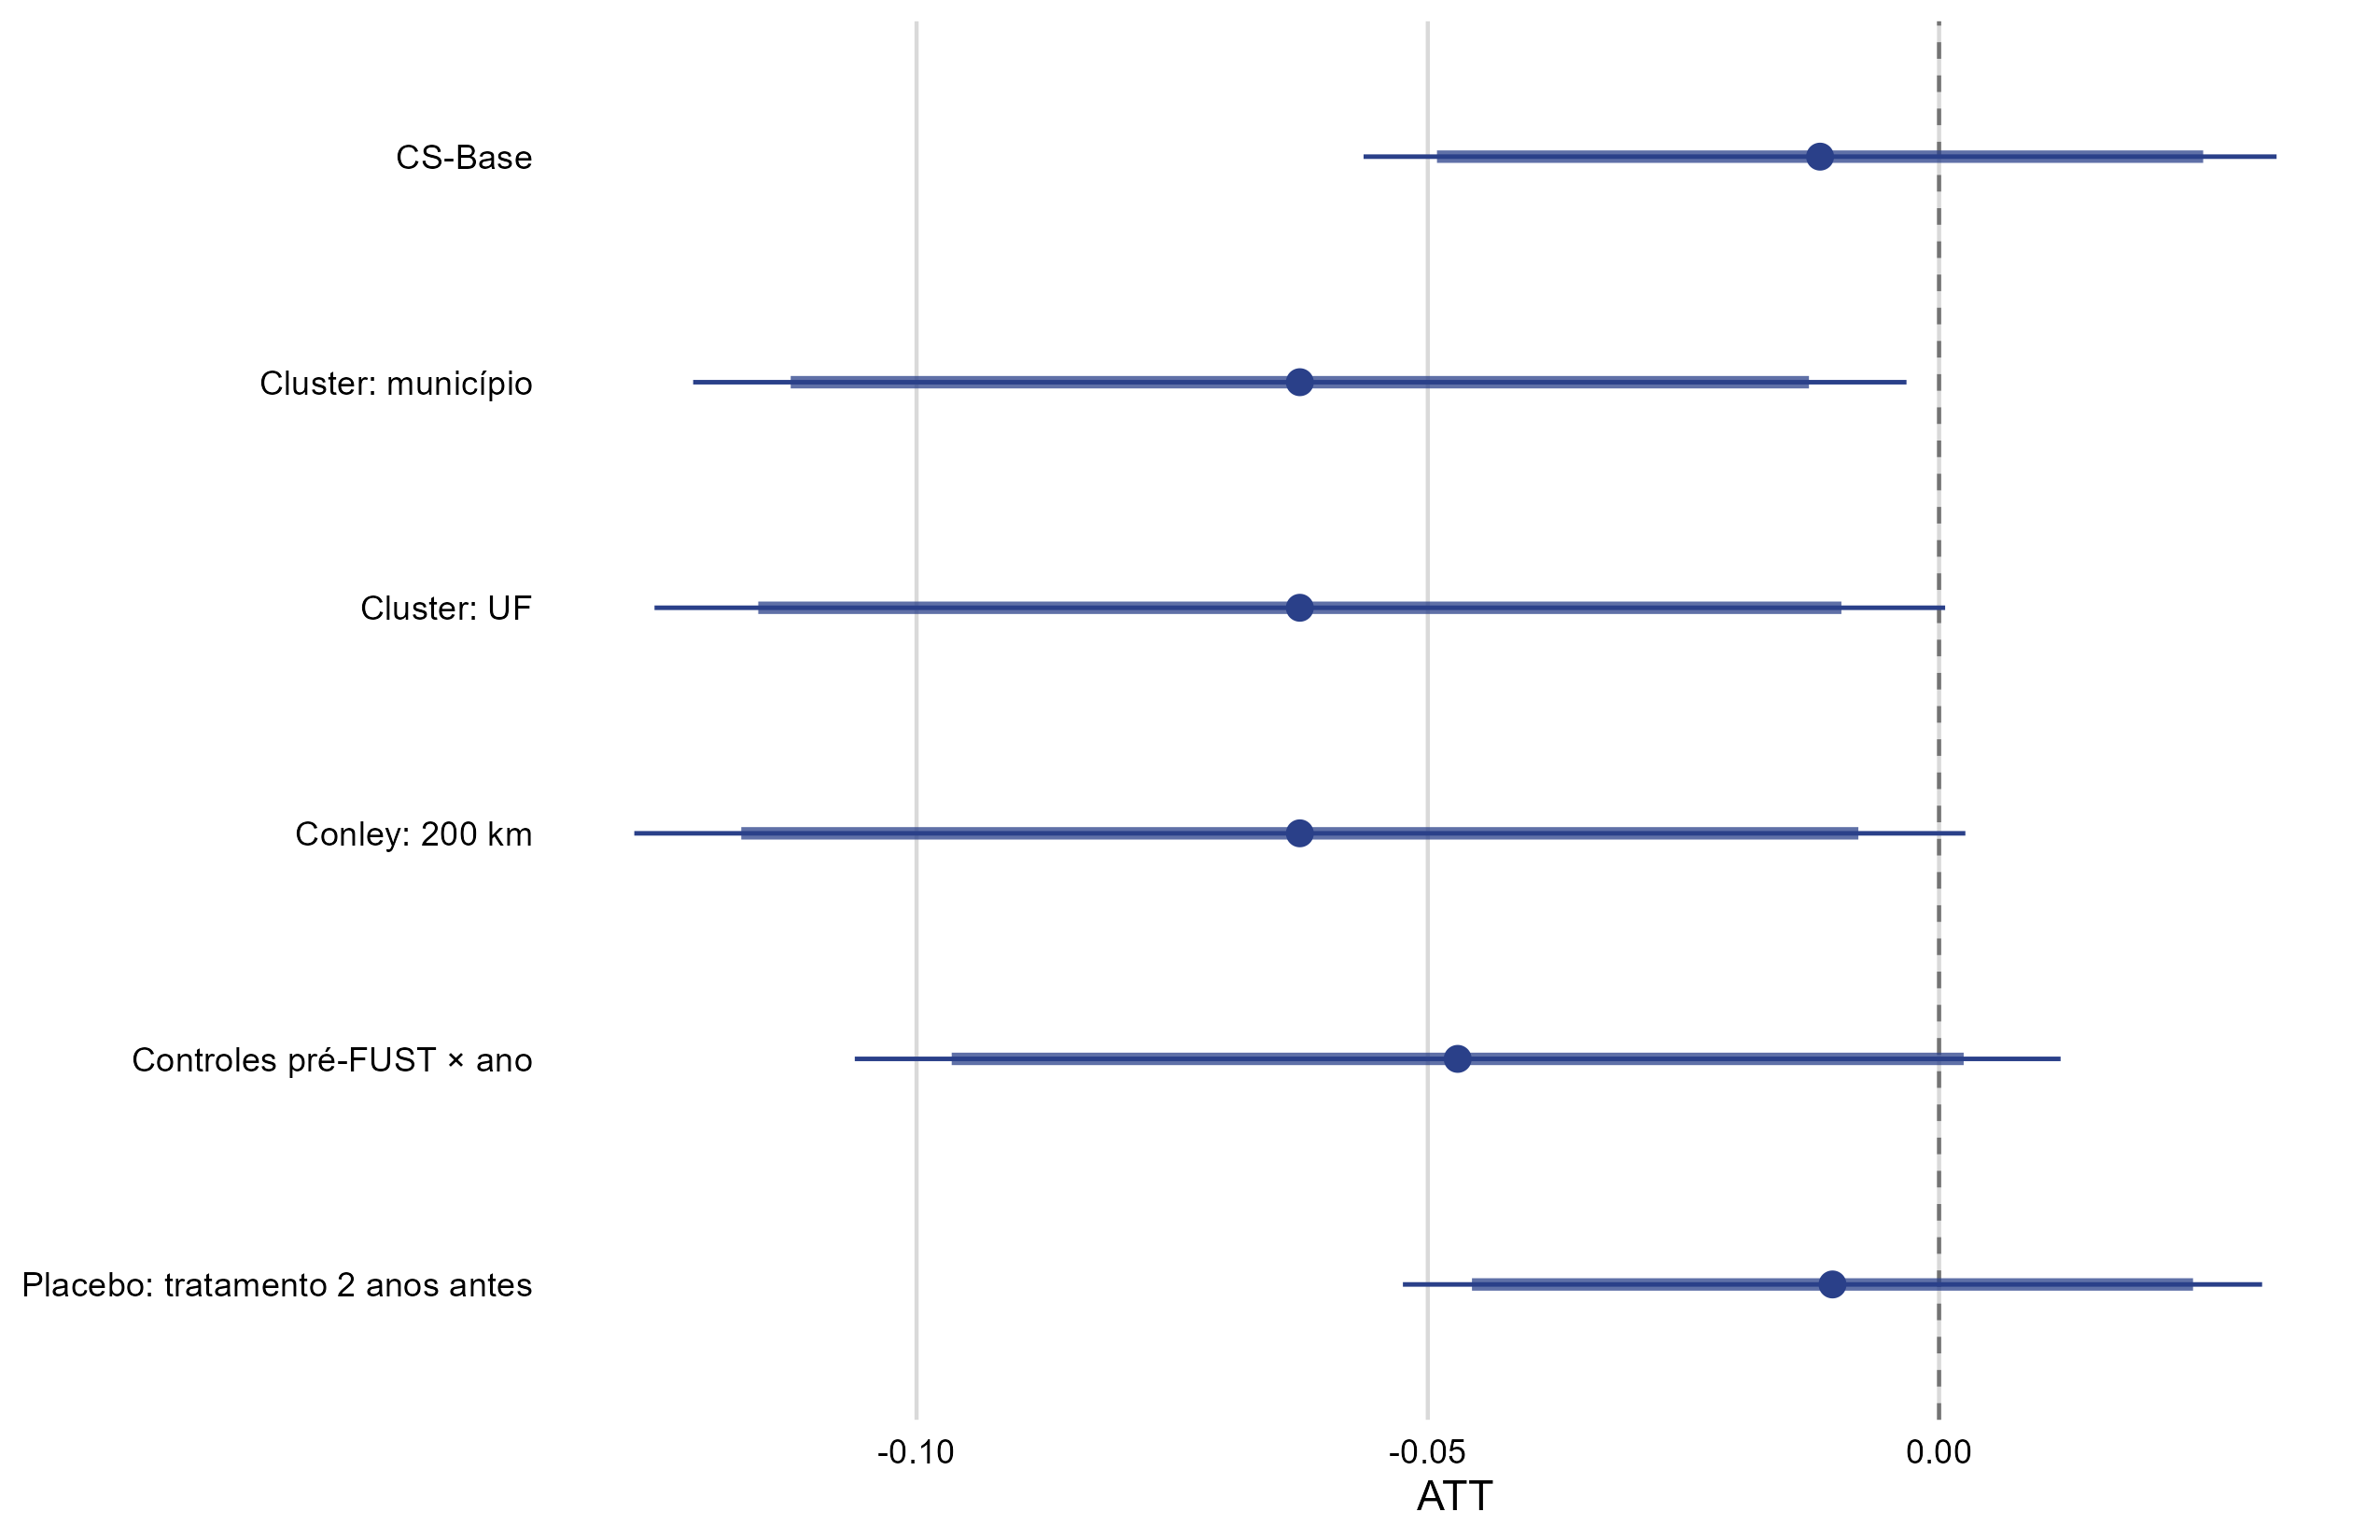
\includegraphics[width=0.96\textwidth]{Robustez - Log-salario-medio.png}
\caption{Robustez geral: salário médio}
\label{fig:rob_geral_salario}
\figurenote{Barras grossas e finas: intervalos de 90\% e 95\%. A linha CS-Base usa o estimador
principal; as linhas de agrupamento, Conley e controles usam TWFE.}
\end{figure}

\clearpage
\subsection{Especificações alternativas de pareamento}

São consideradas quatro alternativas: vizinho mais próximo com reposição, entropy matching,
painel balanceado e propensity score 1:1. O emprego é extremamente estável: os ATTs médios ficam
entre 0,231 e 0,235 e são significativos em todas as alternativas. A massa salarial permanece
positiva, com estimativas entre 0,414 e 0,557. O salário médio continua nulo em três alternativas;
no painel balanceado, surge efeito negativo de $-0,036$ ($p=0{,}015$).

Os testes conjuntos de pré-tendências seguem um padrão importante: não rejeitam para massa
salarial, mas rejeitam para emprego e salário médio em todas as regras de pareamento. Assim, a
estabilidade das magnitudes não substitui a análise de sensibilidade a desvios de tendências
paralelas.

\begin{figure}[p]
\centering
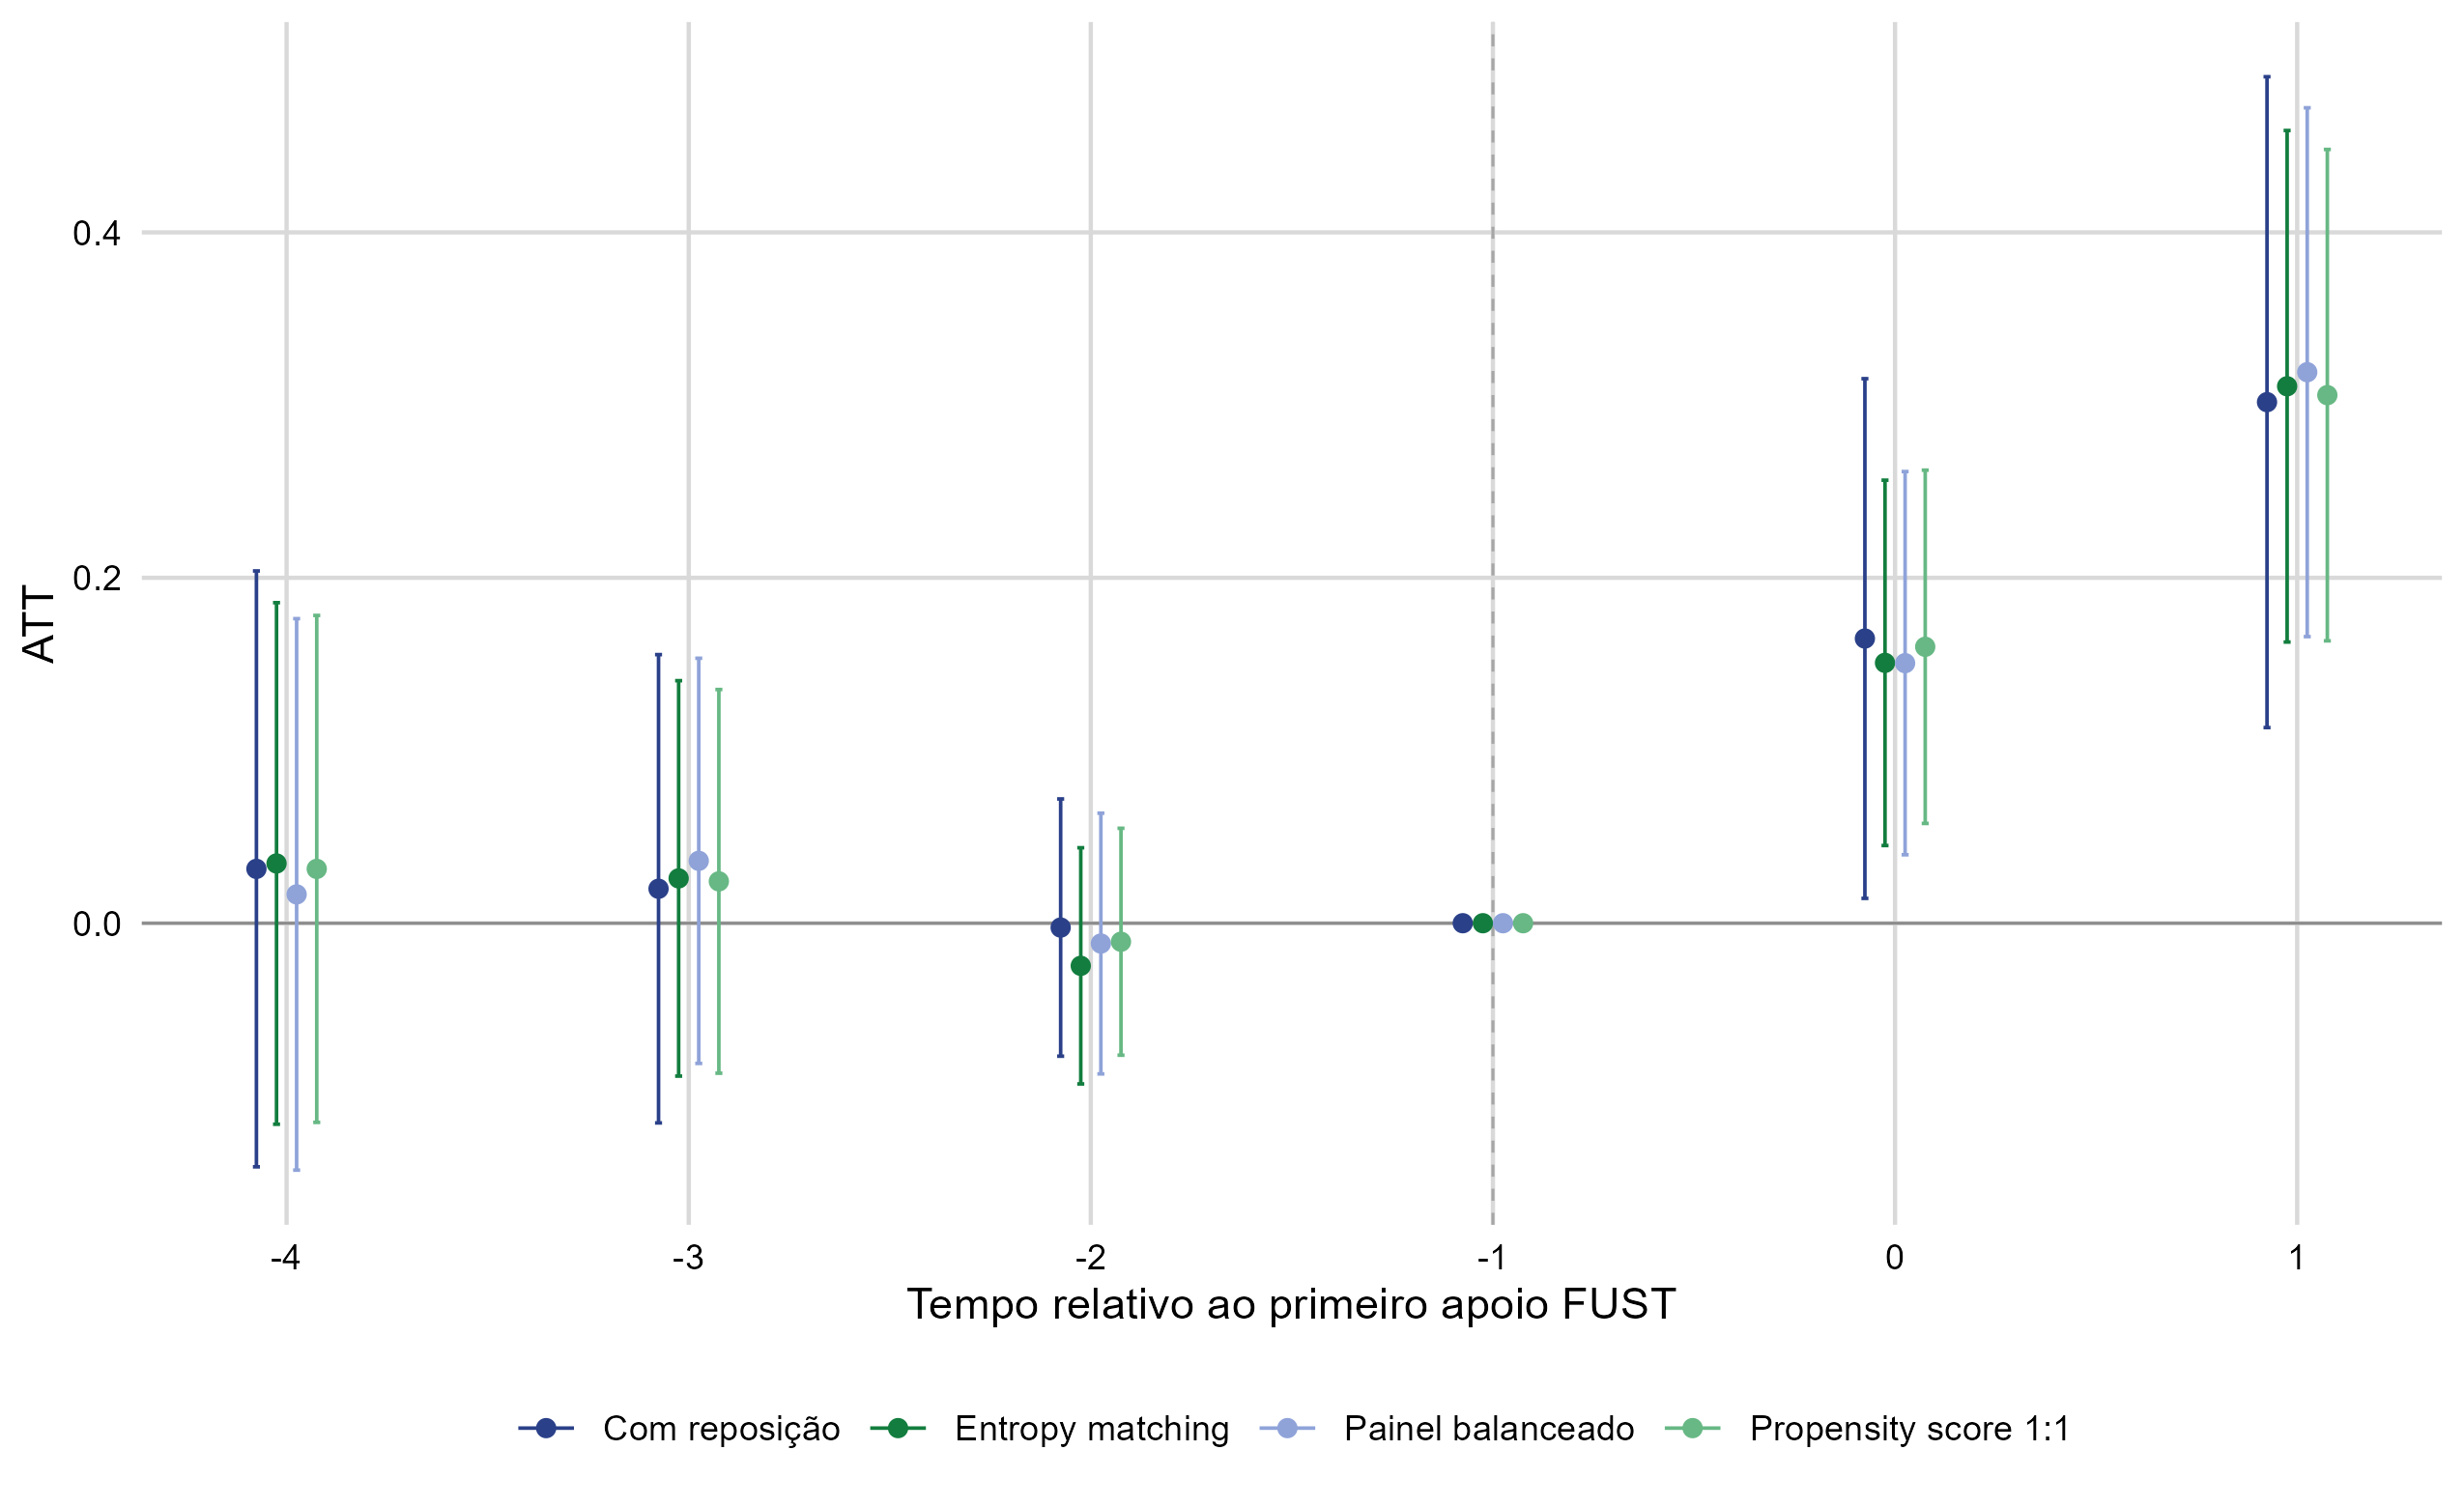
\includegraphics[width=0.96\textwidth]{Robustez - Especificacoes de matching - Event study - Log-emprego.png}
\caption{Pareamentos alternativos: emprego}
\label{fig:rob_match_emp}
\figurenote{Estudos de evento sob quatro regras alternativas de construção do grupo de controle;
intervalos pontuais de 95\%.}
\end{figure}

\begin{figure}[p]
\centering
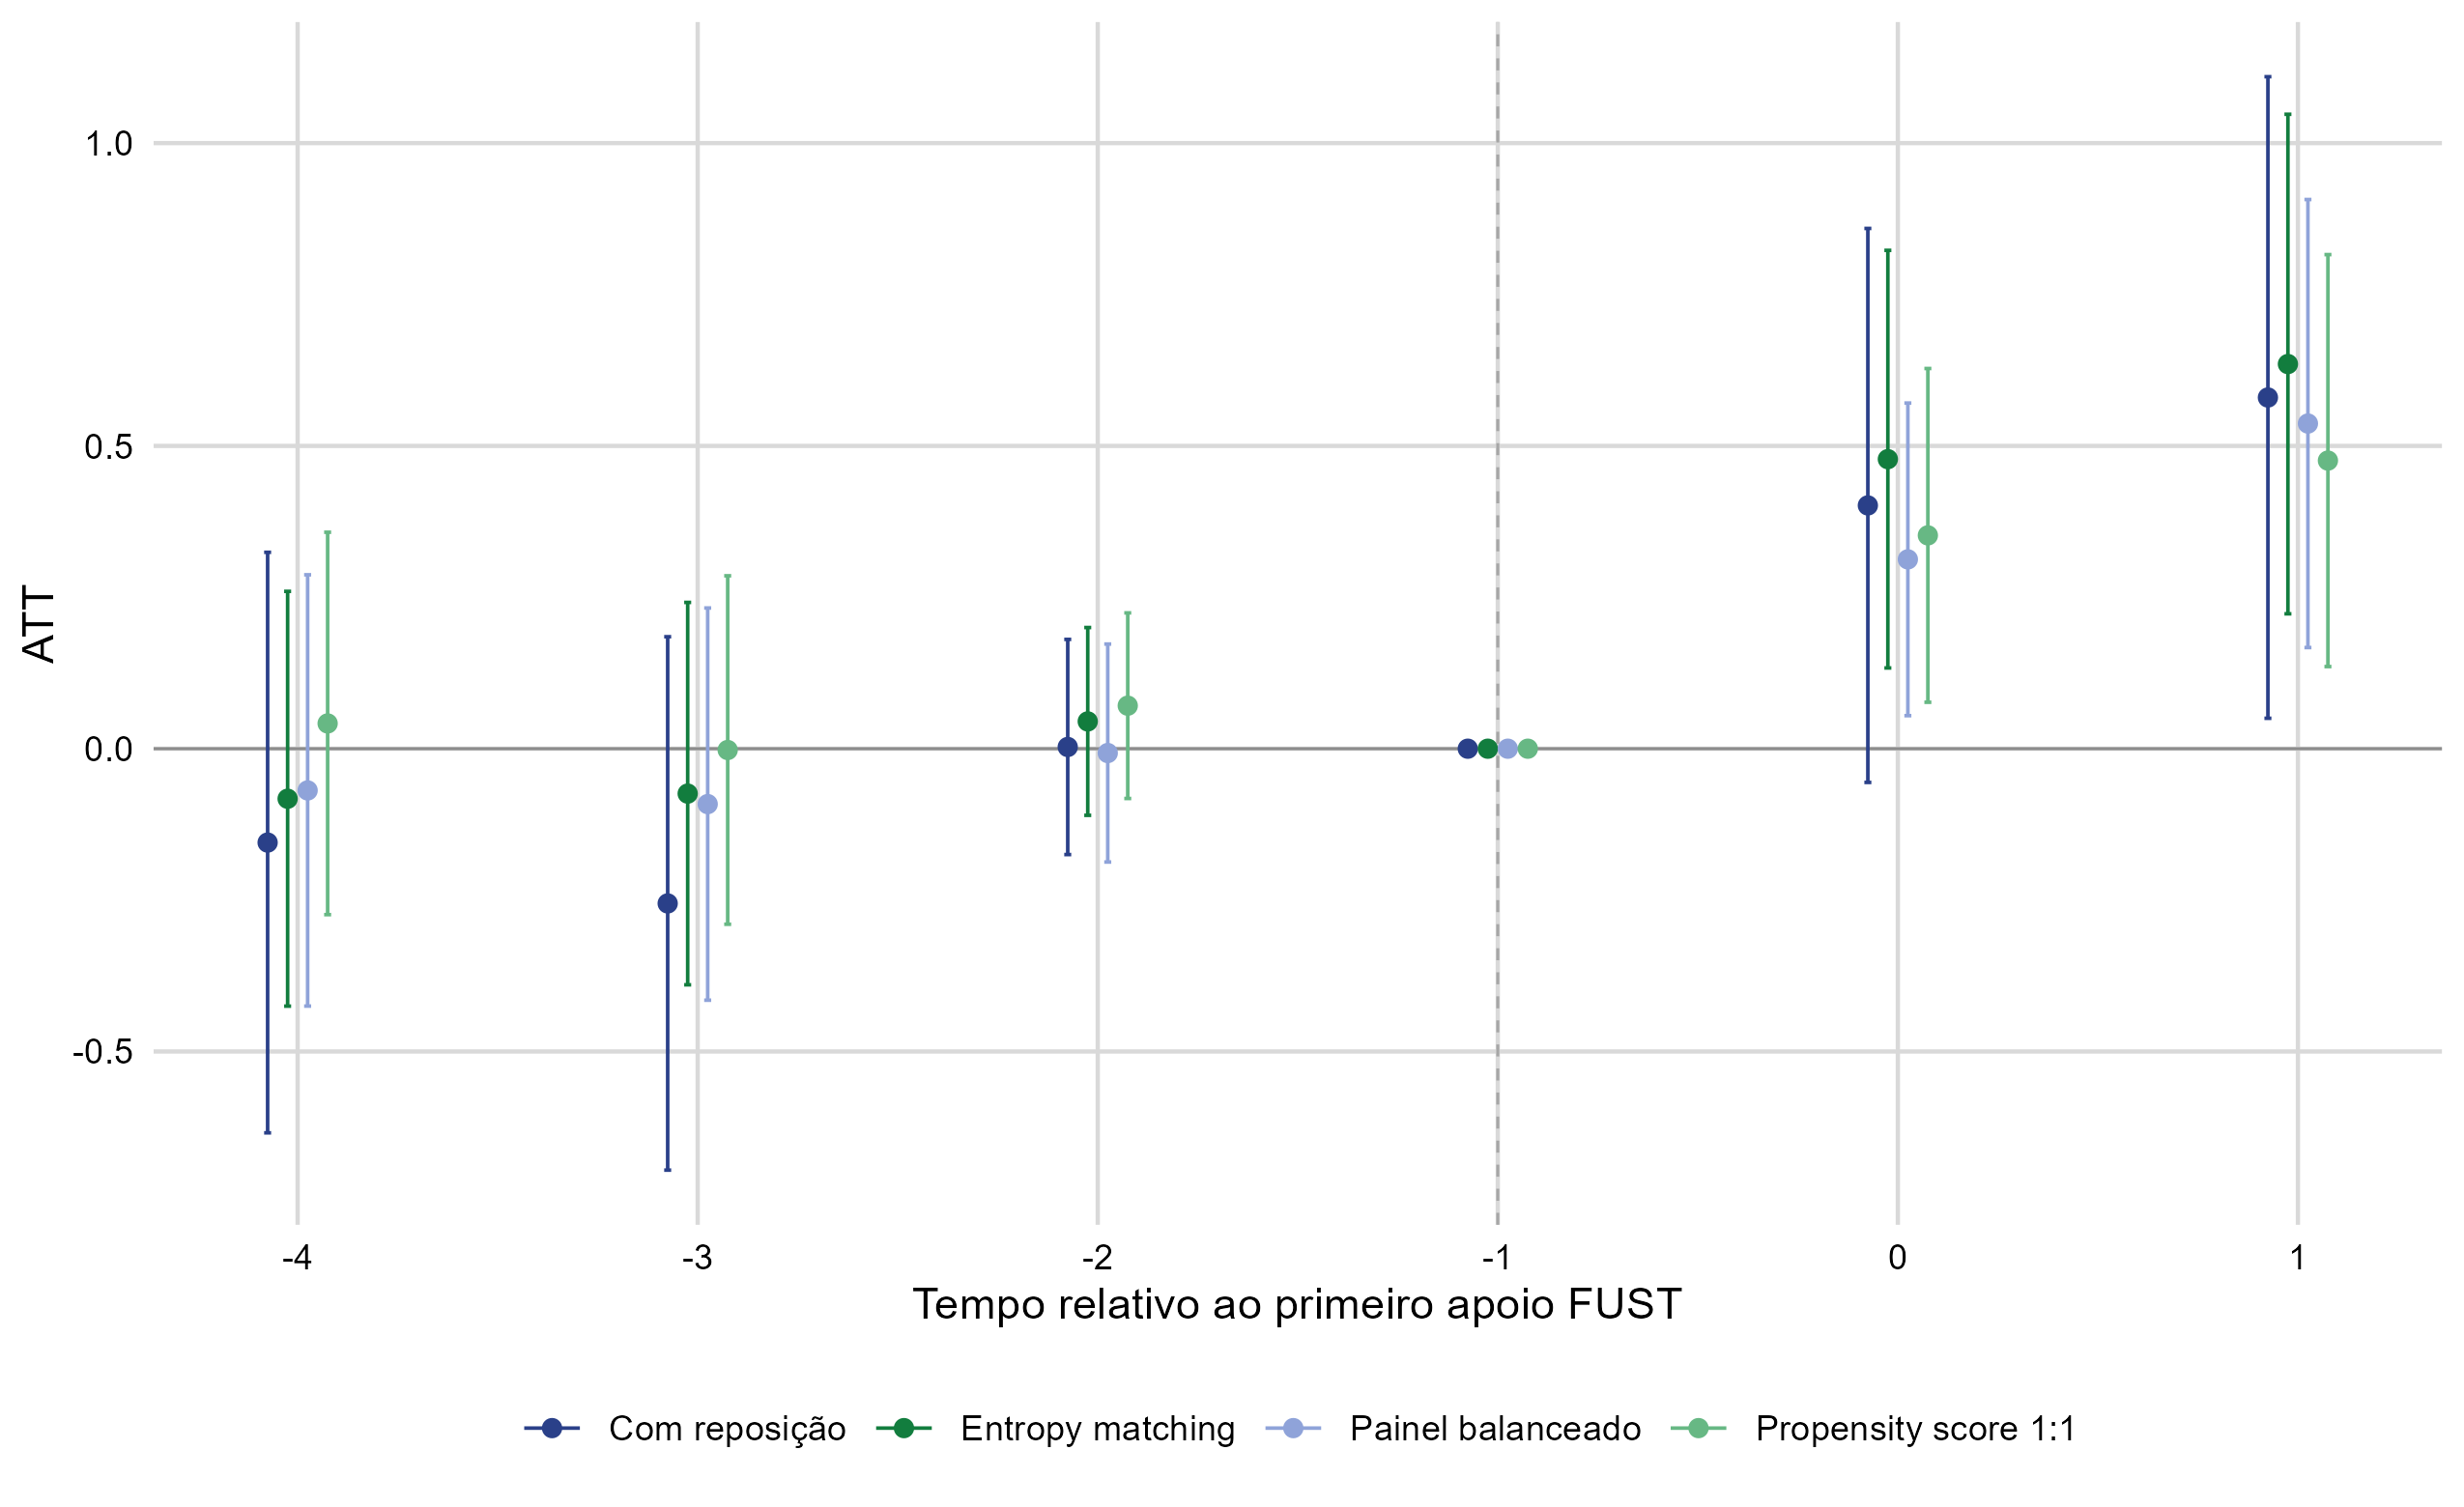
\includegraphics[width=0.96\textwidth]{Robustez - Especificacoes de matching - Event study - Log-massa-salarial.png}
\caption{Pareamentos alternativos: massa salarial}
\label{fig:rob_match_massa}
\figurenote{Estudos de evento sob quatro regras alternativas de construção do grupo de controle;
intervalos pontuais de 95\%.}
\end{figure}

\begin{figure}[p]
\centering
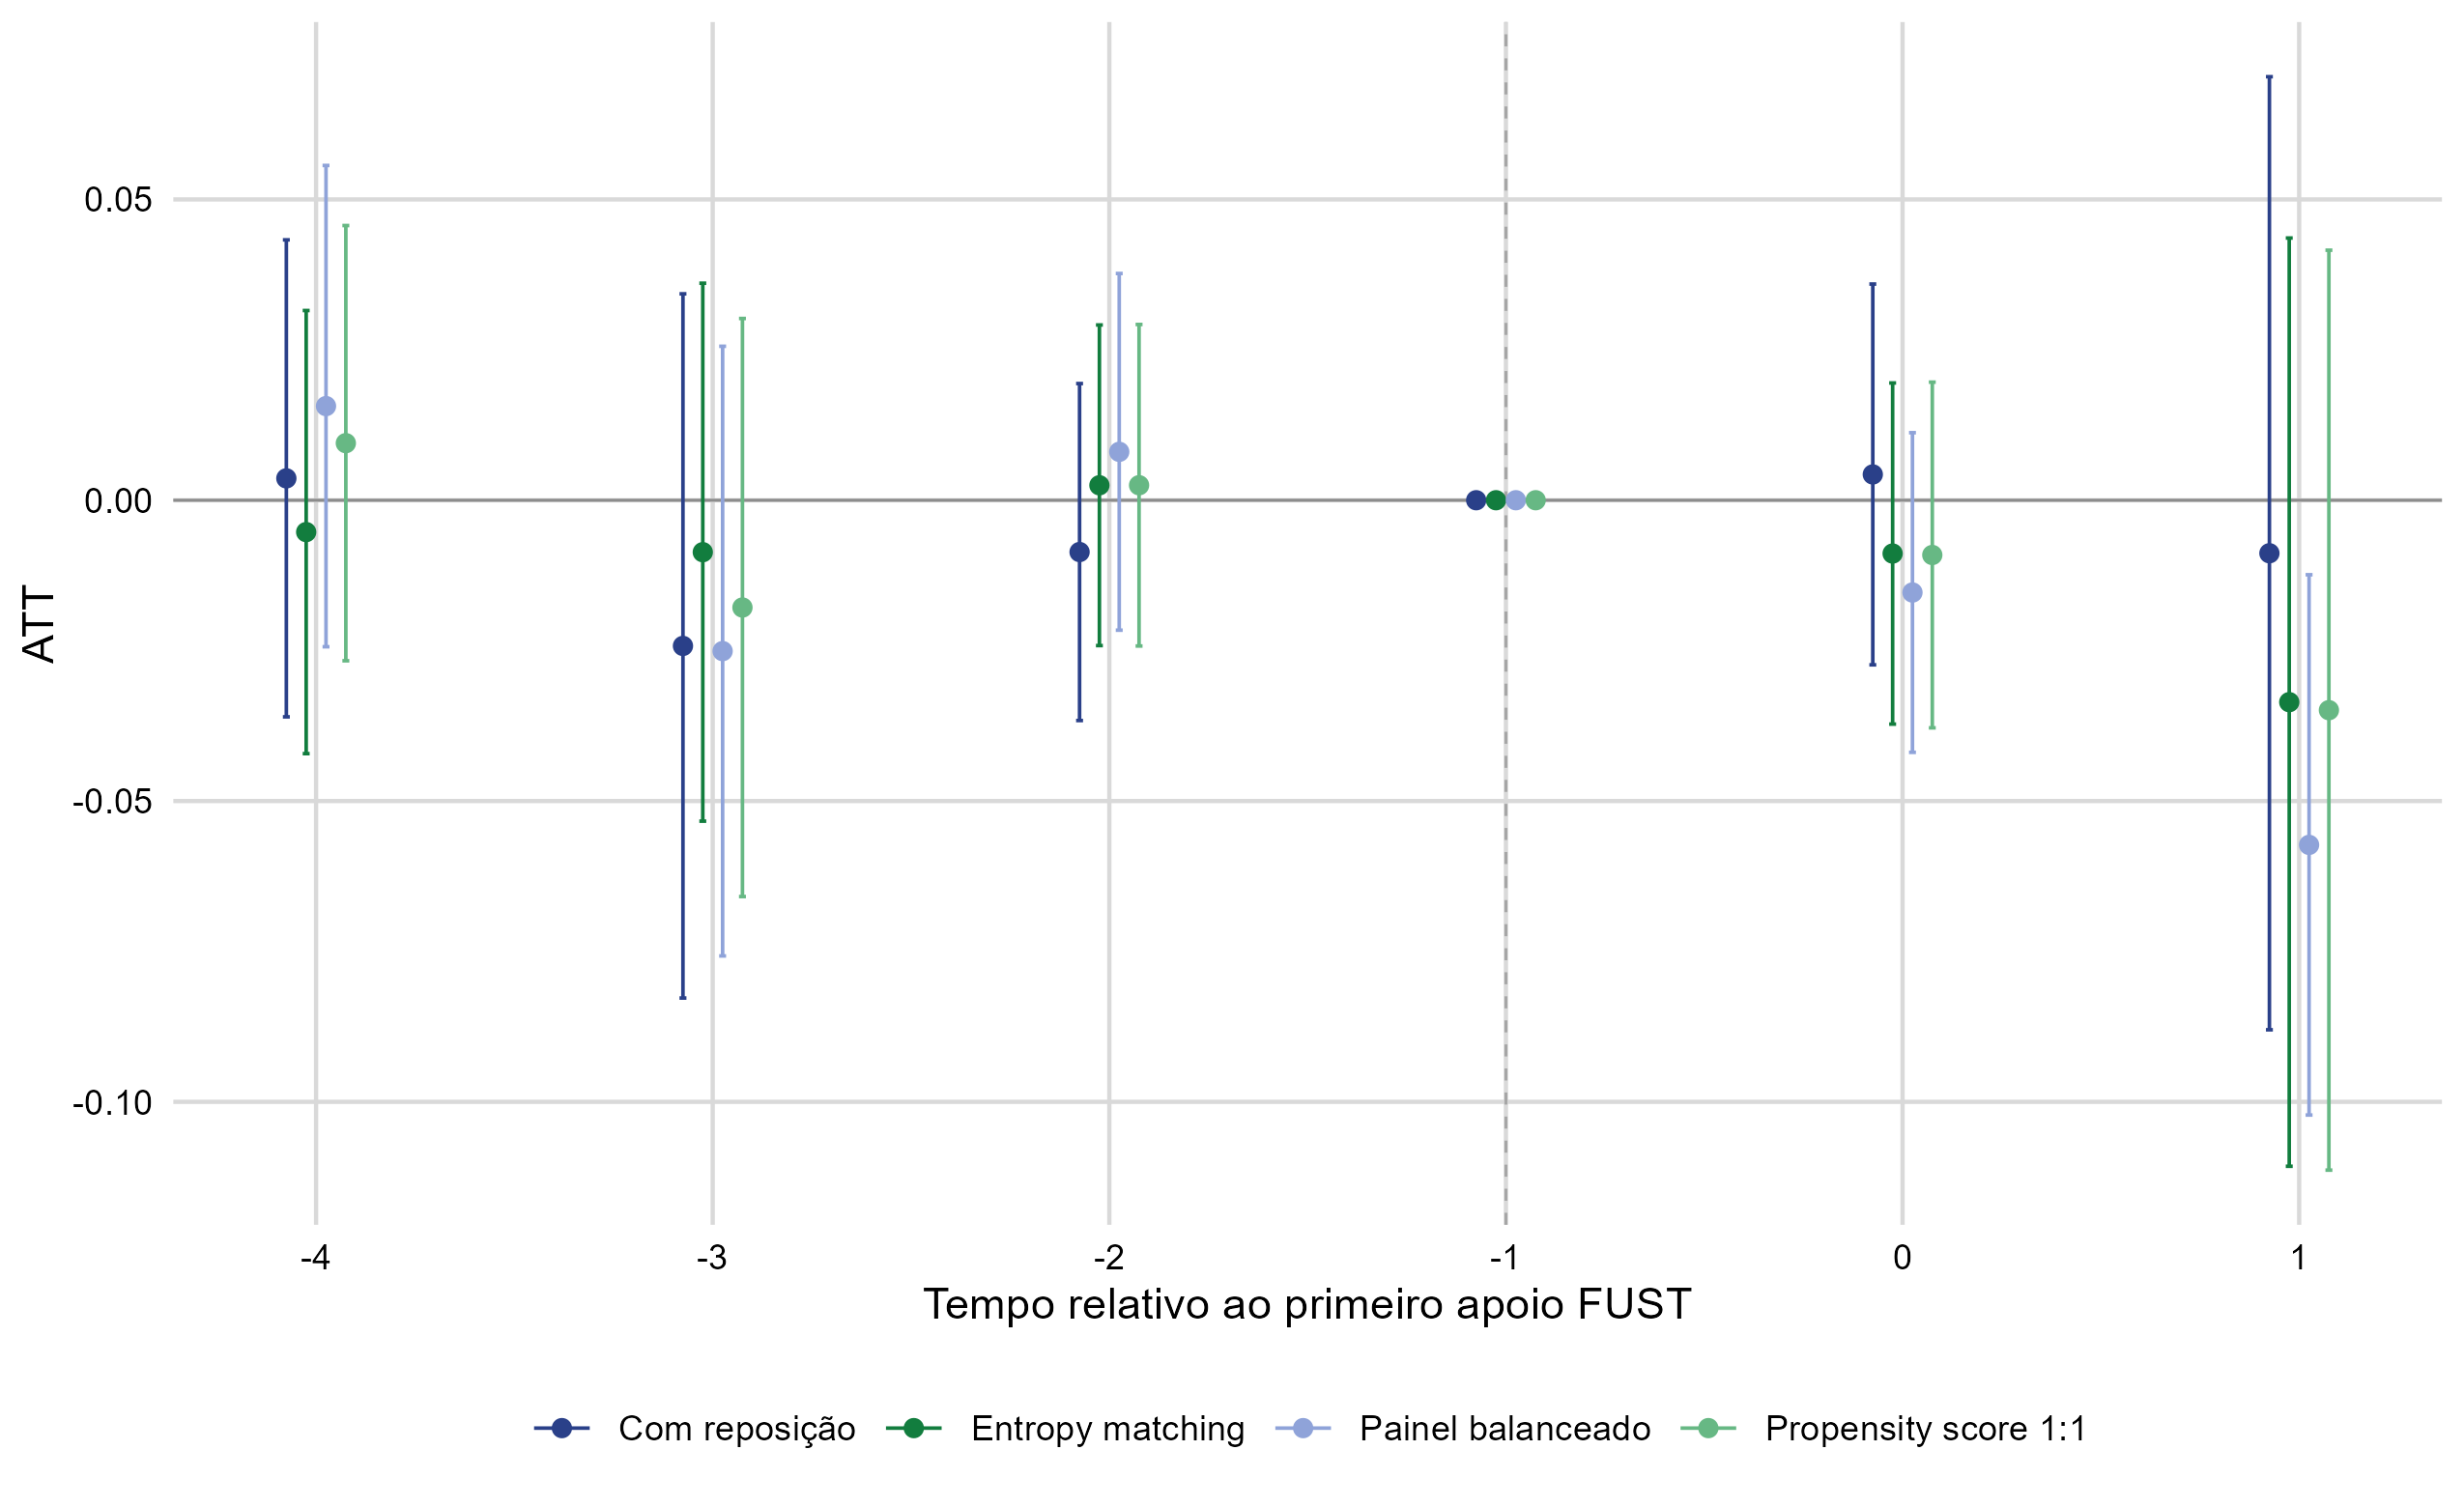
\includegraphics[width=0.96\textwidth]{Robustez - Especificacoes de matching - Event study - Log-salario-medio.png}
\caption{Pareamentos alternativos: salário médio}
\label{fig:rob_match_salario}
\figurenote{Estudos de evento sob quatro regras alternativas de construção do grupo de controle;
intervalos pontuais de 95\%.}
\end{figure}

\clearpage
\subsection{Estimadores alternativos}

Os resultados são reestimados por efeitos fixos de duas vias (TWFE), Gardner/did2s,
Borusyak--Jaravel--Spiess por imputação e diferença-em-diferenças sintética (SDID). Para emprego,
todos apontam efeito contemporâneo entre 0,130 e 0,140 e crescimento no ano seguinte, entre 0,325
e 0,522. Para massa salarial, o efeito contemporâneo varia entre 0,219 e 0,281 e o efeito em
$e=1$ entre 0,536 e 0,705; a incerteza é maior em $e=0$, mas o segundo horizonte é positivo.

Para salário médio, todos os estimadores produzem efeito contemporâneo pequeno e não
significativo. Em $e=1$, TWFE, Gardner e imputação indicam queda próxima de 0,11 ponto de log;
SDID também é negativo ($-0,058$), mas seu intervalo inclui zero. Esse resultado mostra que a
ausência de efeito no ATT médio principal encobre possível redução no segundo horizonte e reforça
a necessidade de acompanhar coortes por mais anos.

\begin{figure}[p]
\centering
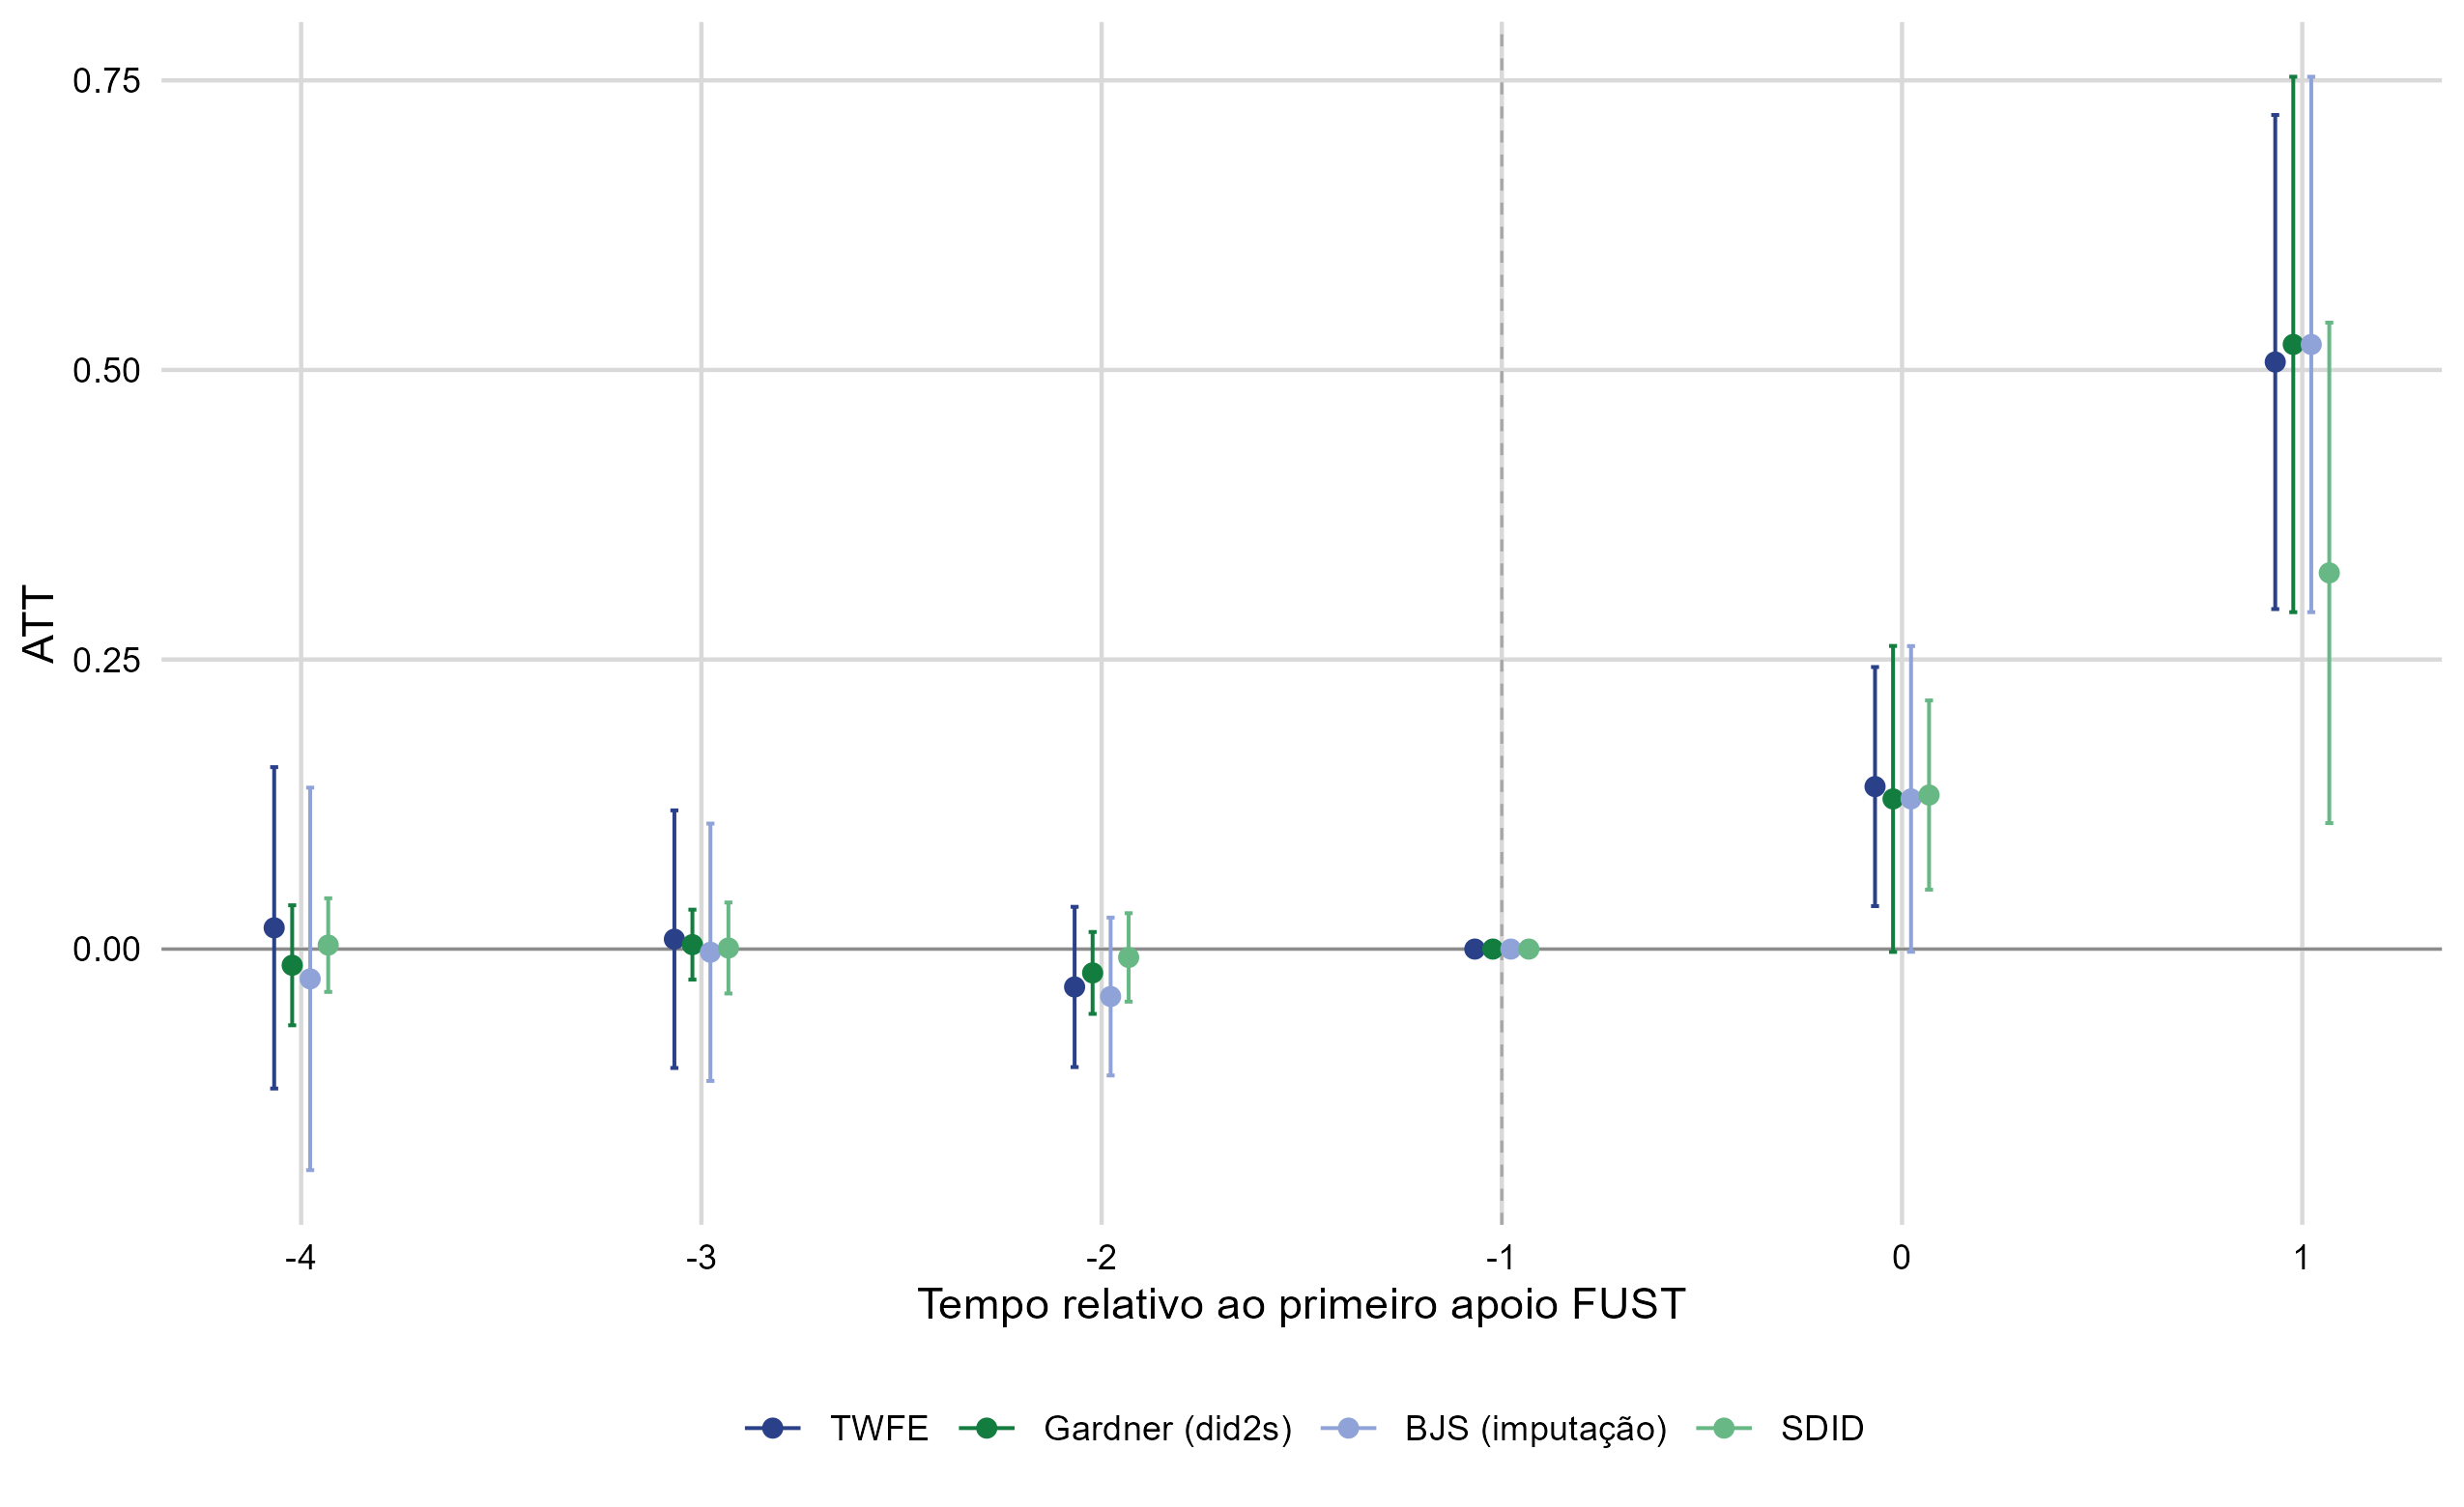
\includegraphics[width=0.96\textwidth]{Robustez - Estimadores - Log-emprego.png}
\caption{Estimadores alternativos: emprego}
\label{fig:rob_est_emp}
\figurenote{TWFE, Gardner/did2s, BJS por imputação e SDID; intervalos pontuais de 95\%.}
\end{figure}

\begin{figure}[p]
\centering
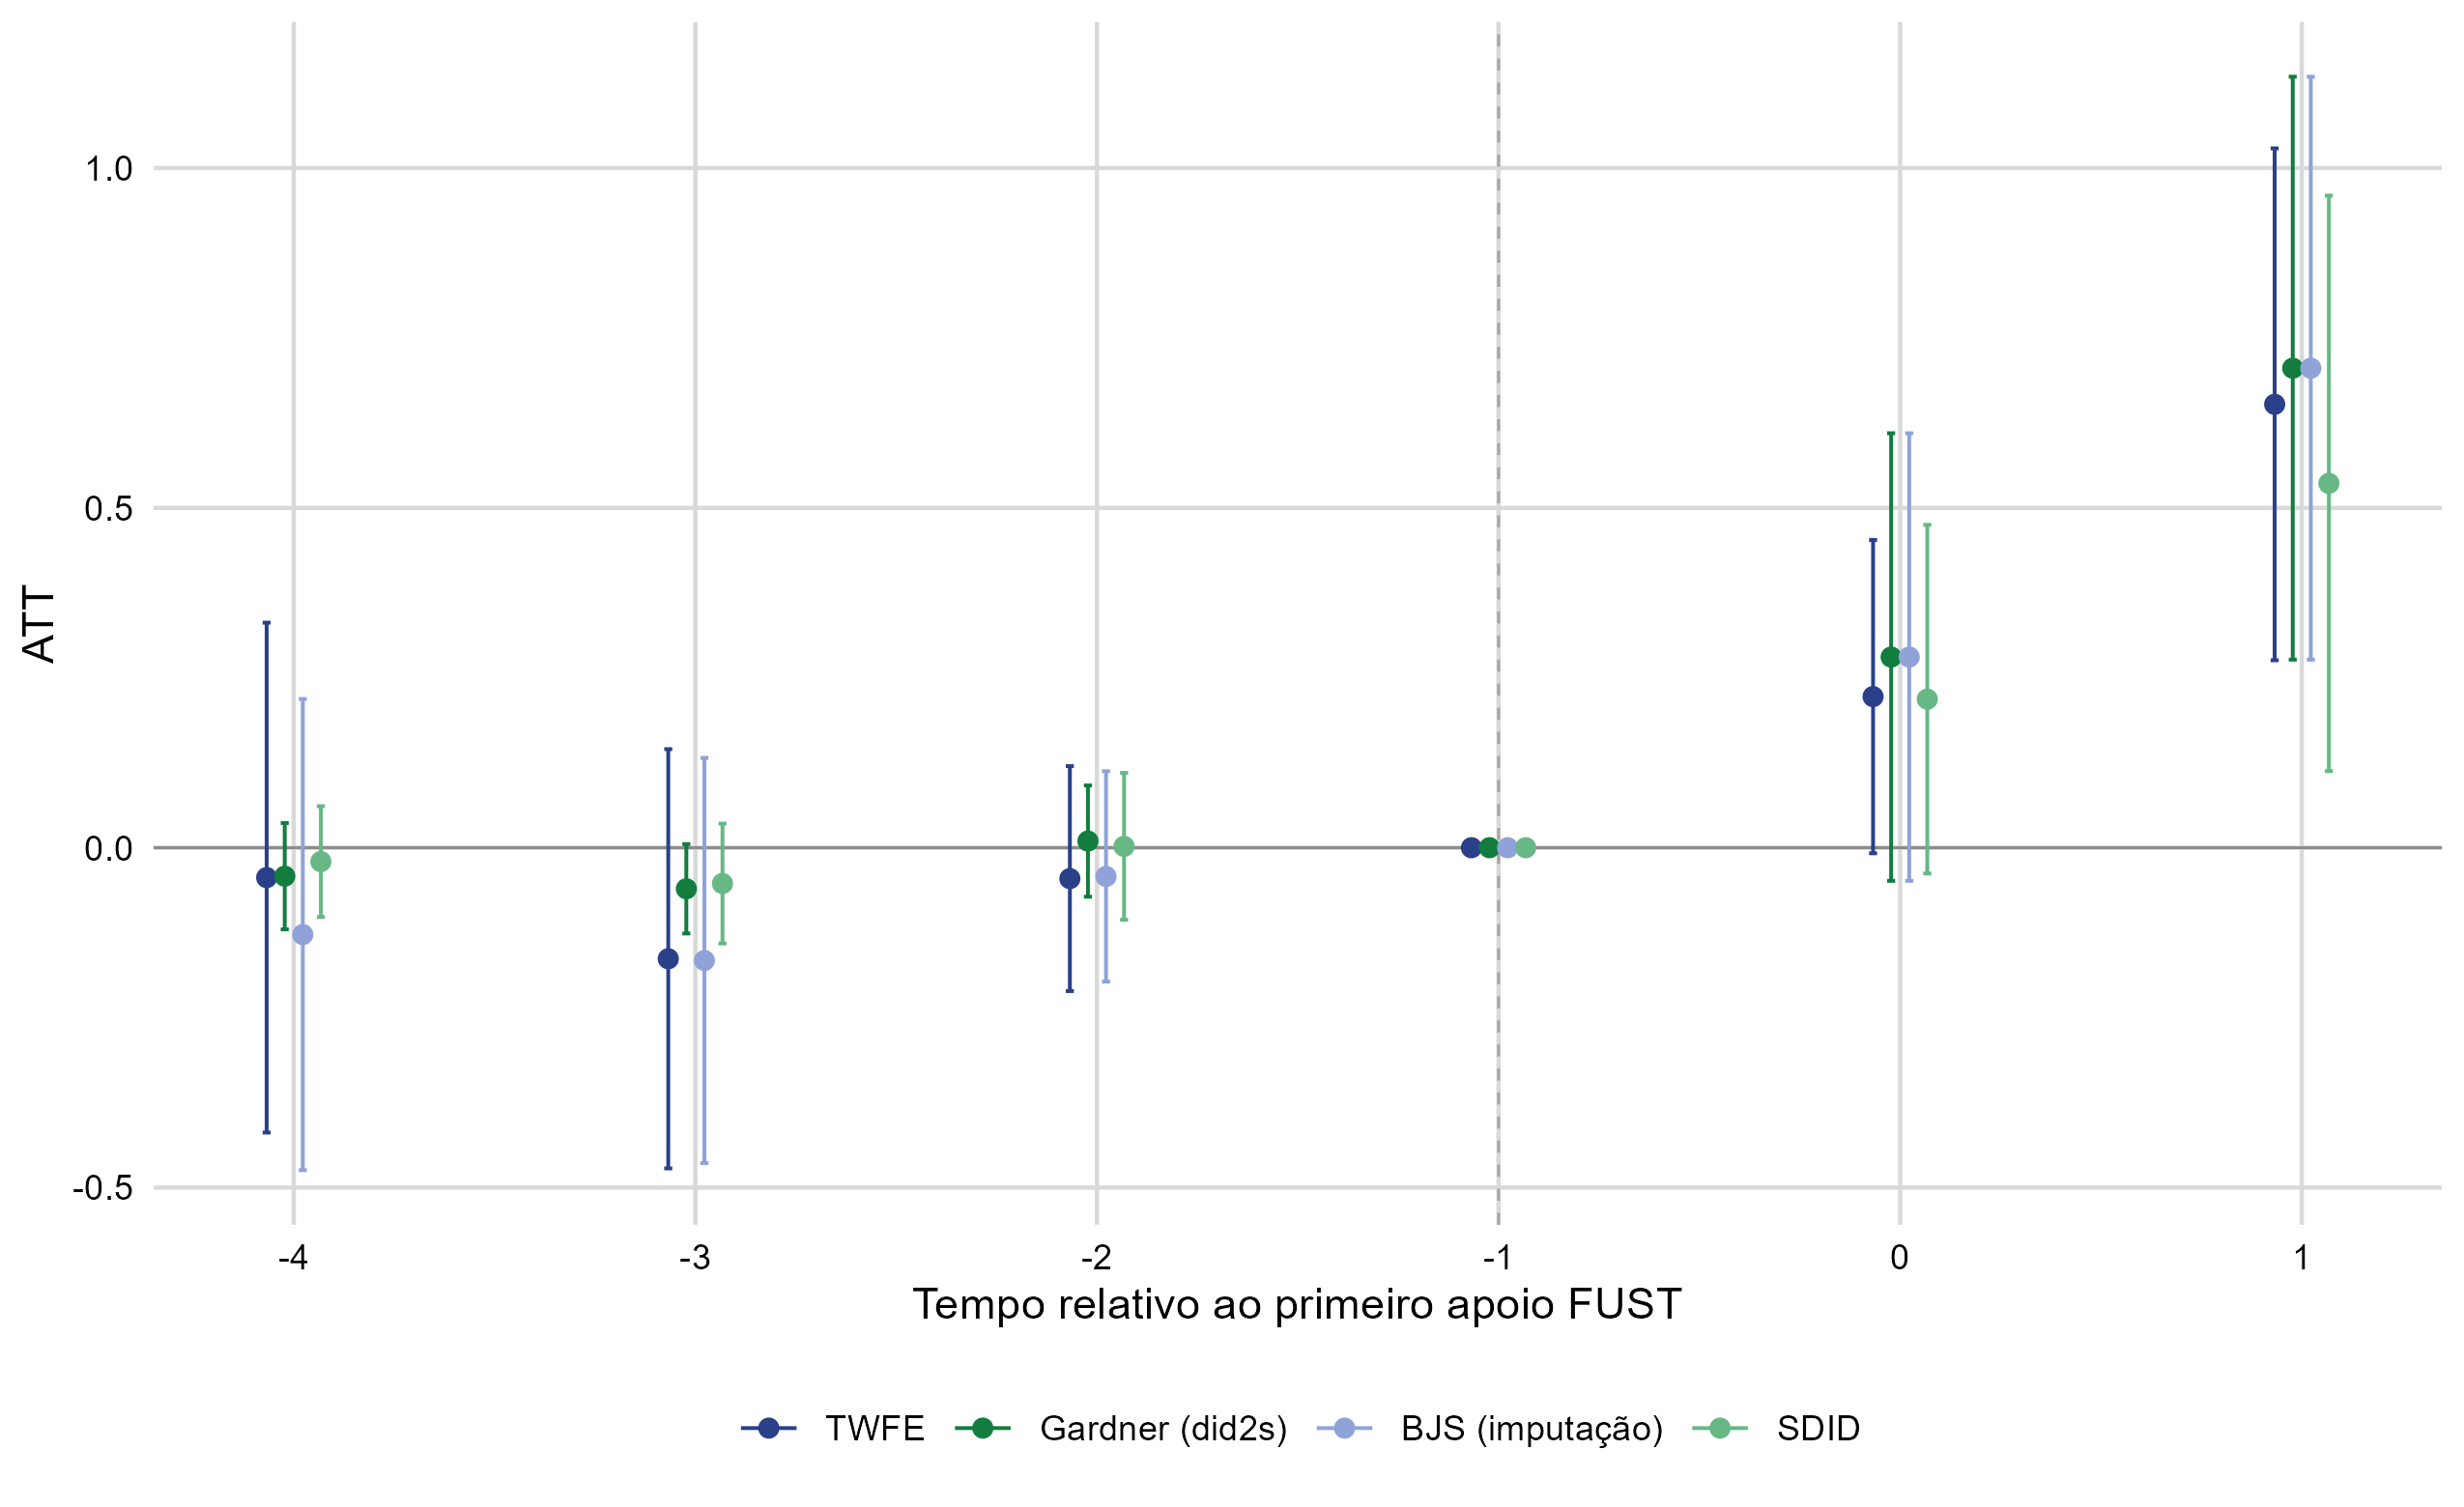
\includegraphics[width=0.96\textwidth]{Robustez - Estimadores - Log-massa-salarial.png}
\caption{Estimadores alternativos: massa salarial}
\label{fig:rob_est_massa}
\figurenote{TWFE, Gardner/did2s, BJS por imputação e SDID; intervalos pontuais de 95\%.}
\end{figure}

\begin{figure}[p]
\centering
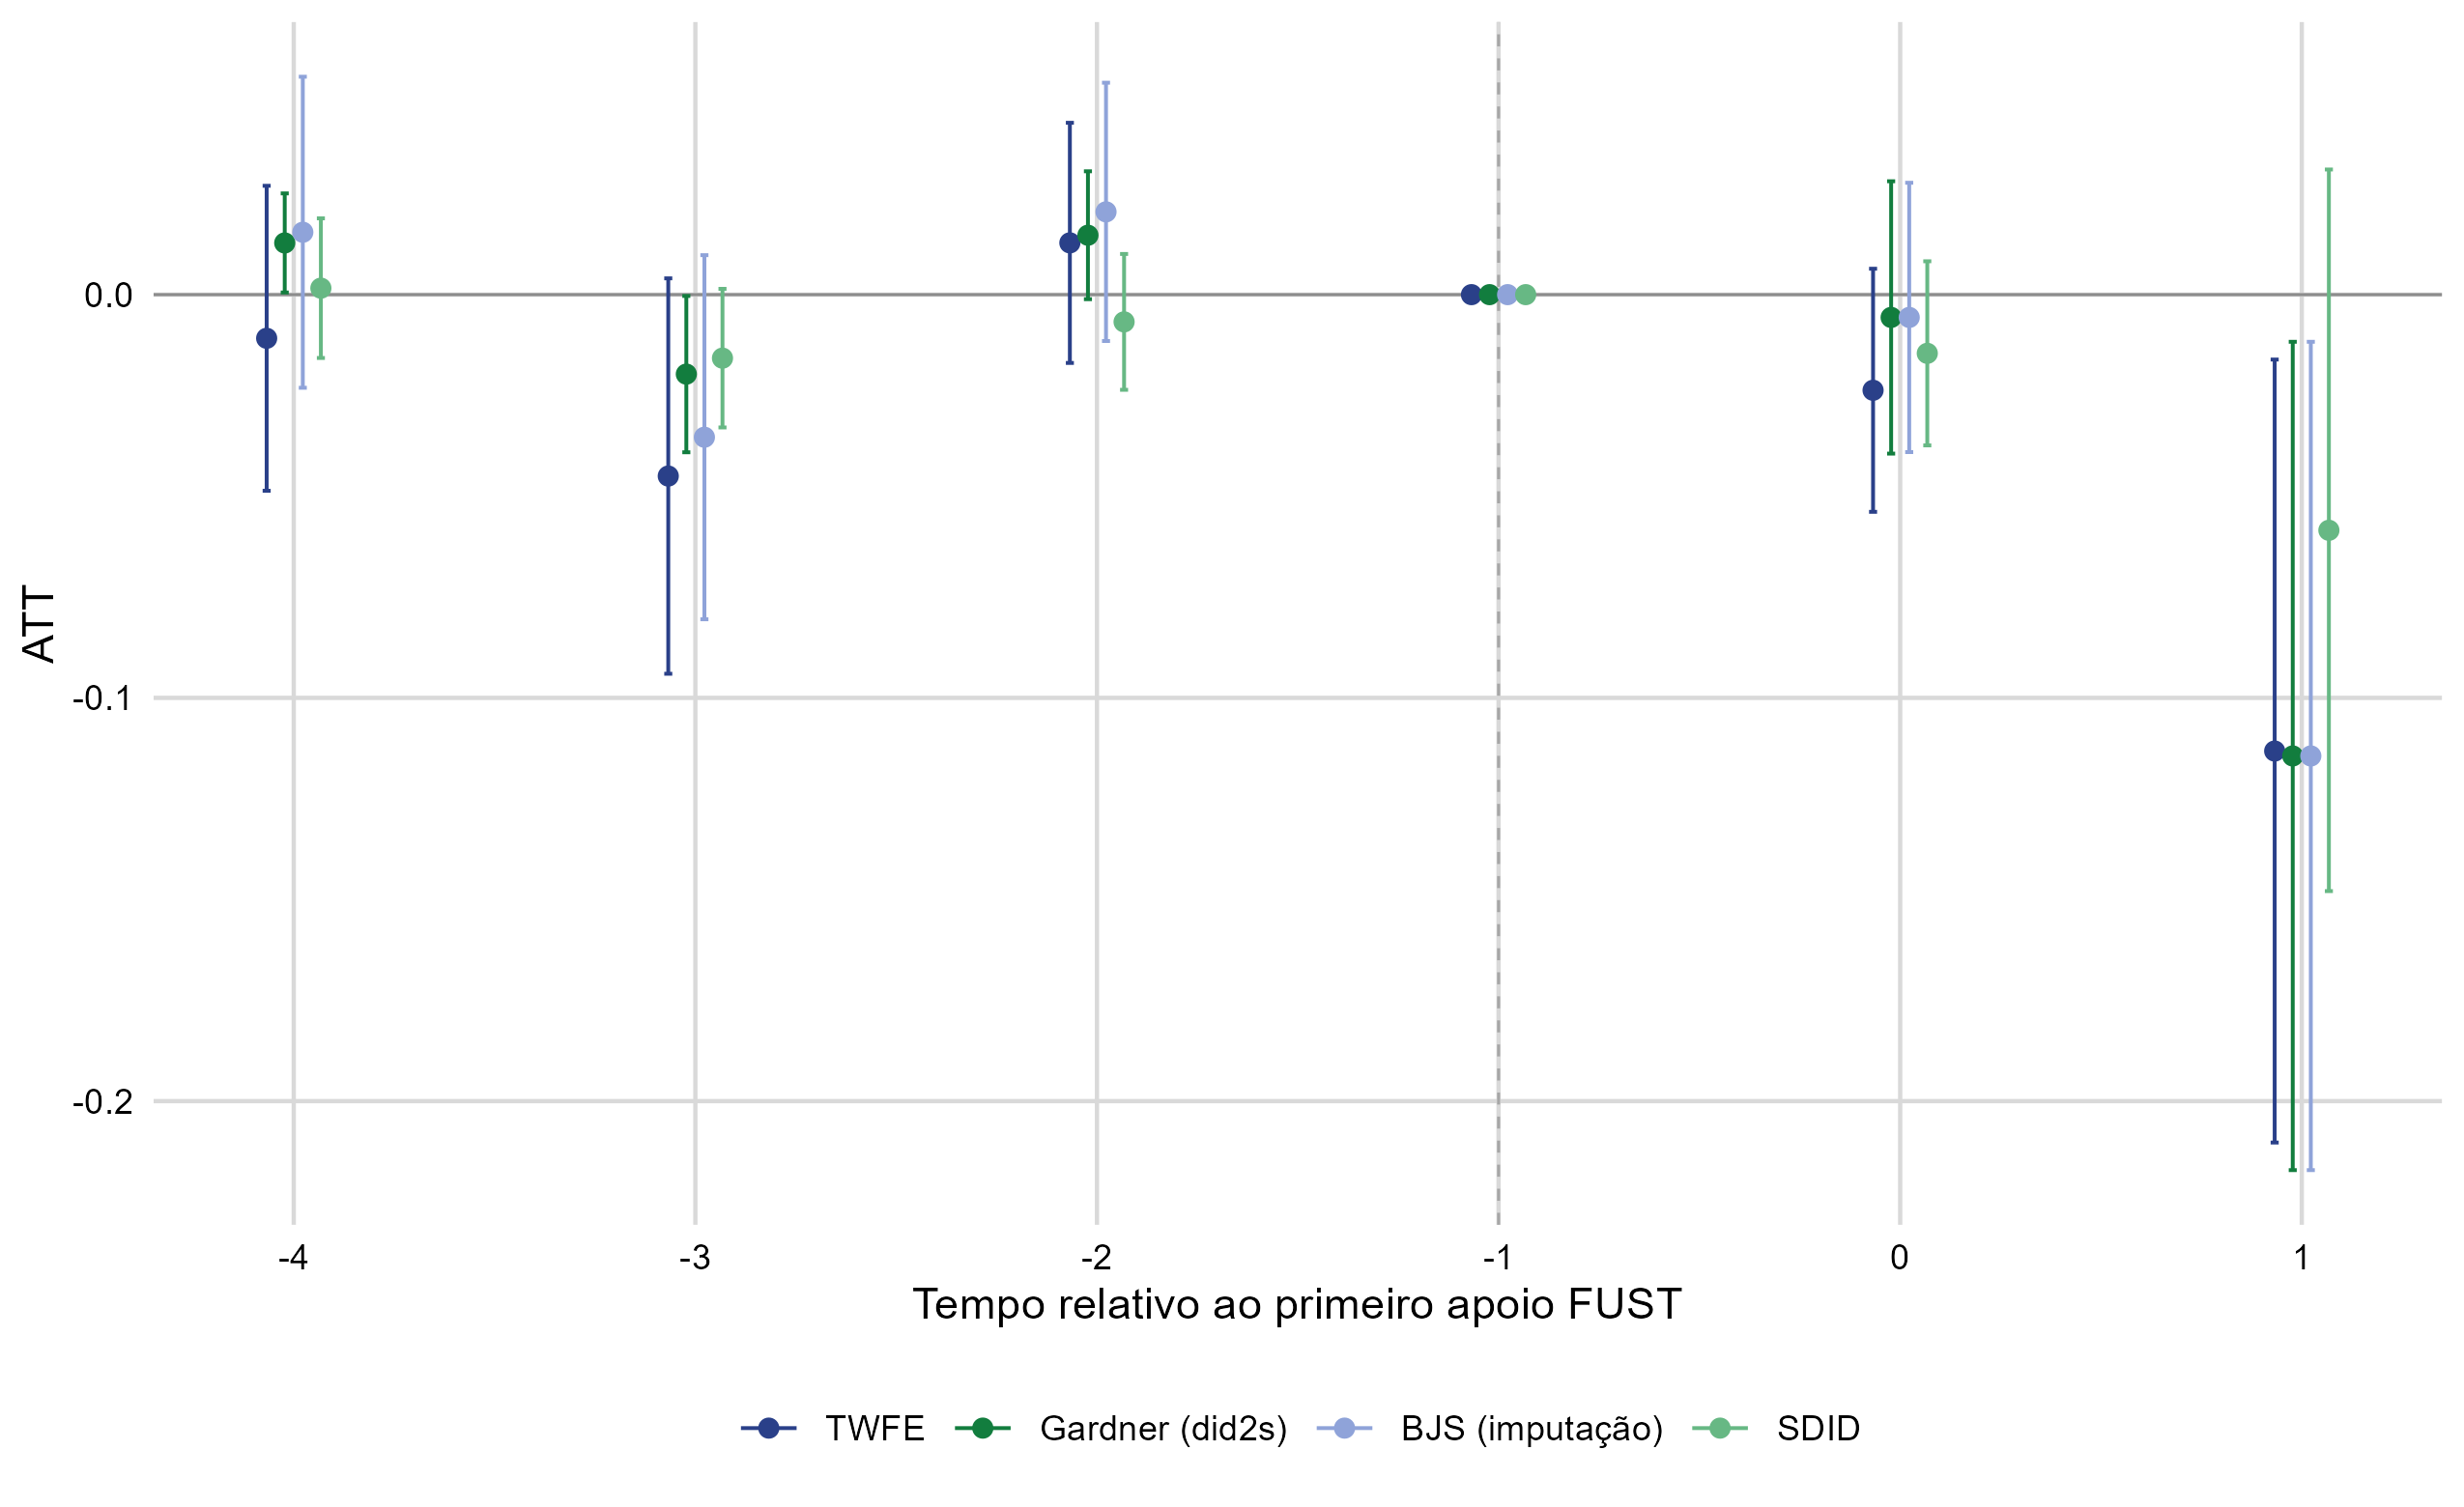
\includegraphics[width=0.96\textwidth]{Robustez - Estimadores - Log-salario-medio.png}
\caption{Estimadores alternativos: salário médio}
\label{fig:rob_est_salario}
\figurenote{TWFE, Gardner/did2s, BJS por imputação e SDID; intervalos pontuais de 95\%.}
\end{figure}

\clearpage
\subsection{HonestDiD}

O HonestDiD de Rambachan--Roth constrói intervalos robustos permitindo que a violação
pós-tratamento das tendências paralelas seja até $\bar M$ vezes a maior violação observada antes
do tratamento. Valores maiores de $\bar M$ representam desvios mais severos.

O efeito médio de emprego permanece positivo mesmo em $\bar M=1$, sinal de robustez substantiva.
Para massa salarial, o limite inferior se aproxima de zero em $\bar M=0{,}7$ e passa a incluir
zero aproximadamente a partir de $\bar M=0{,}8$; o resultado é robusto a violações moderadas, mas
não às mais severas consideradas. Para salário médio, o intervalo original já inclui zero e a
conclusão permanece sem significância em toda a grade.

\begin{figure}[p]
\centering
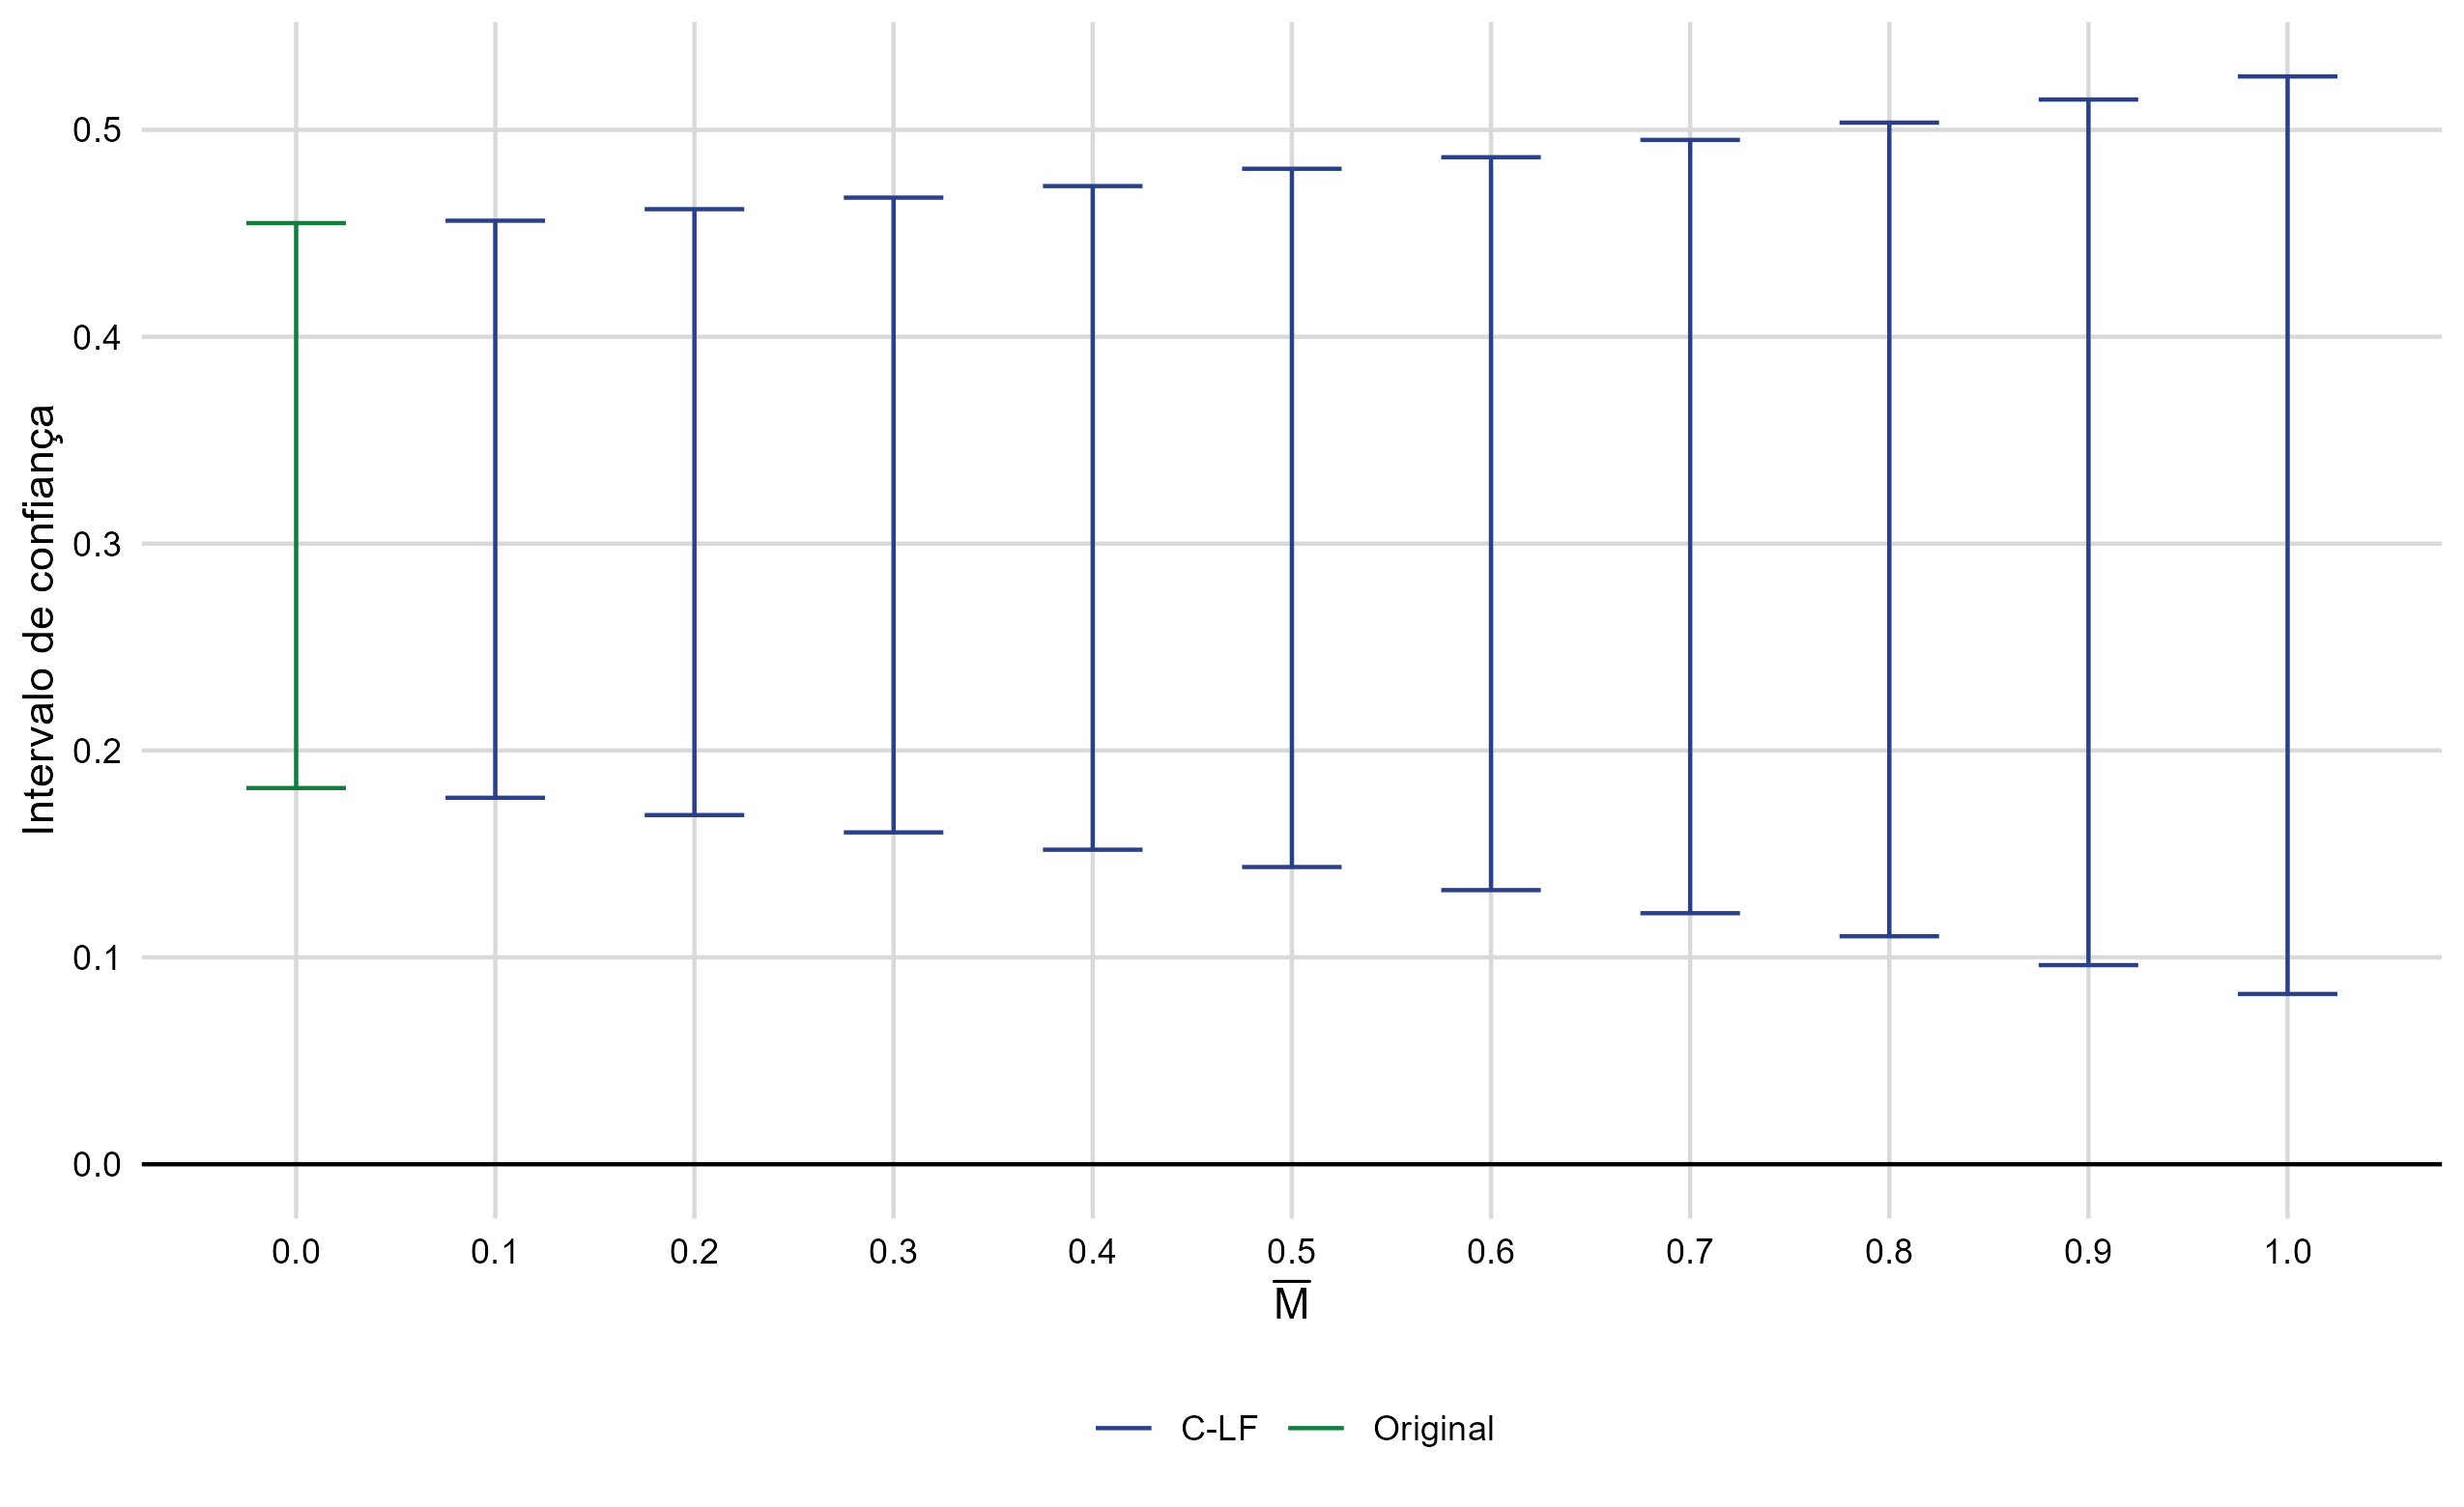
\includegraphics[width=0.96\textwidth]{HonestDiD - Log-emprego.png}
\caption{HonestDiD: emprego}
\label{fig:honest_emp}
\figurenote{Intervalos de confiança robustos a desvios relativos de tendências paralelas. Verde:
intervalo original; azul: intervalo C-LF para cada $\bar M$.}
\end{figure}

\begin{figure}[p]
\centering
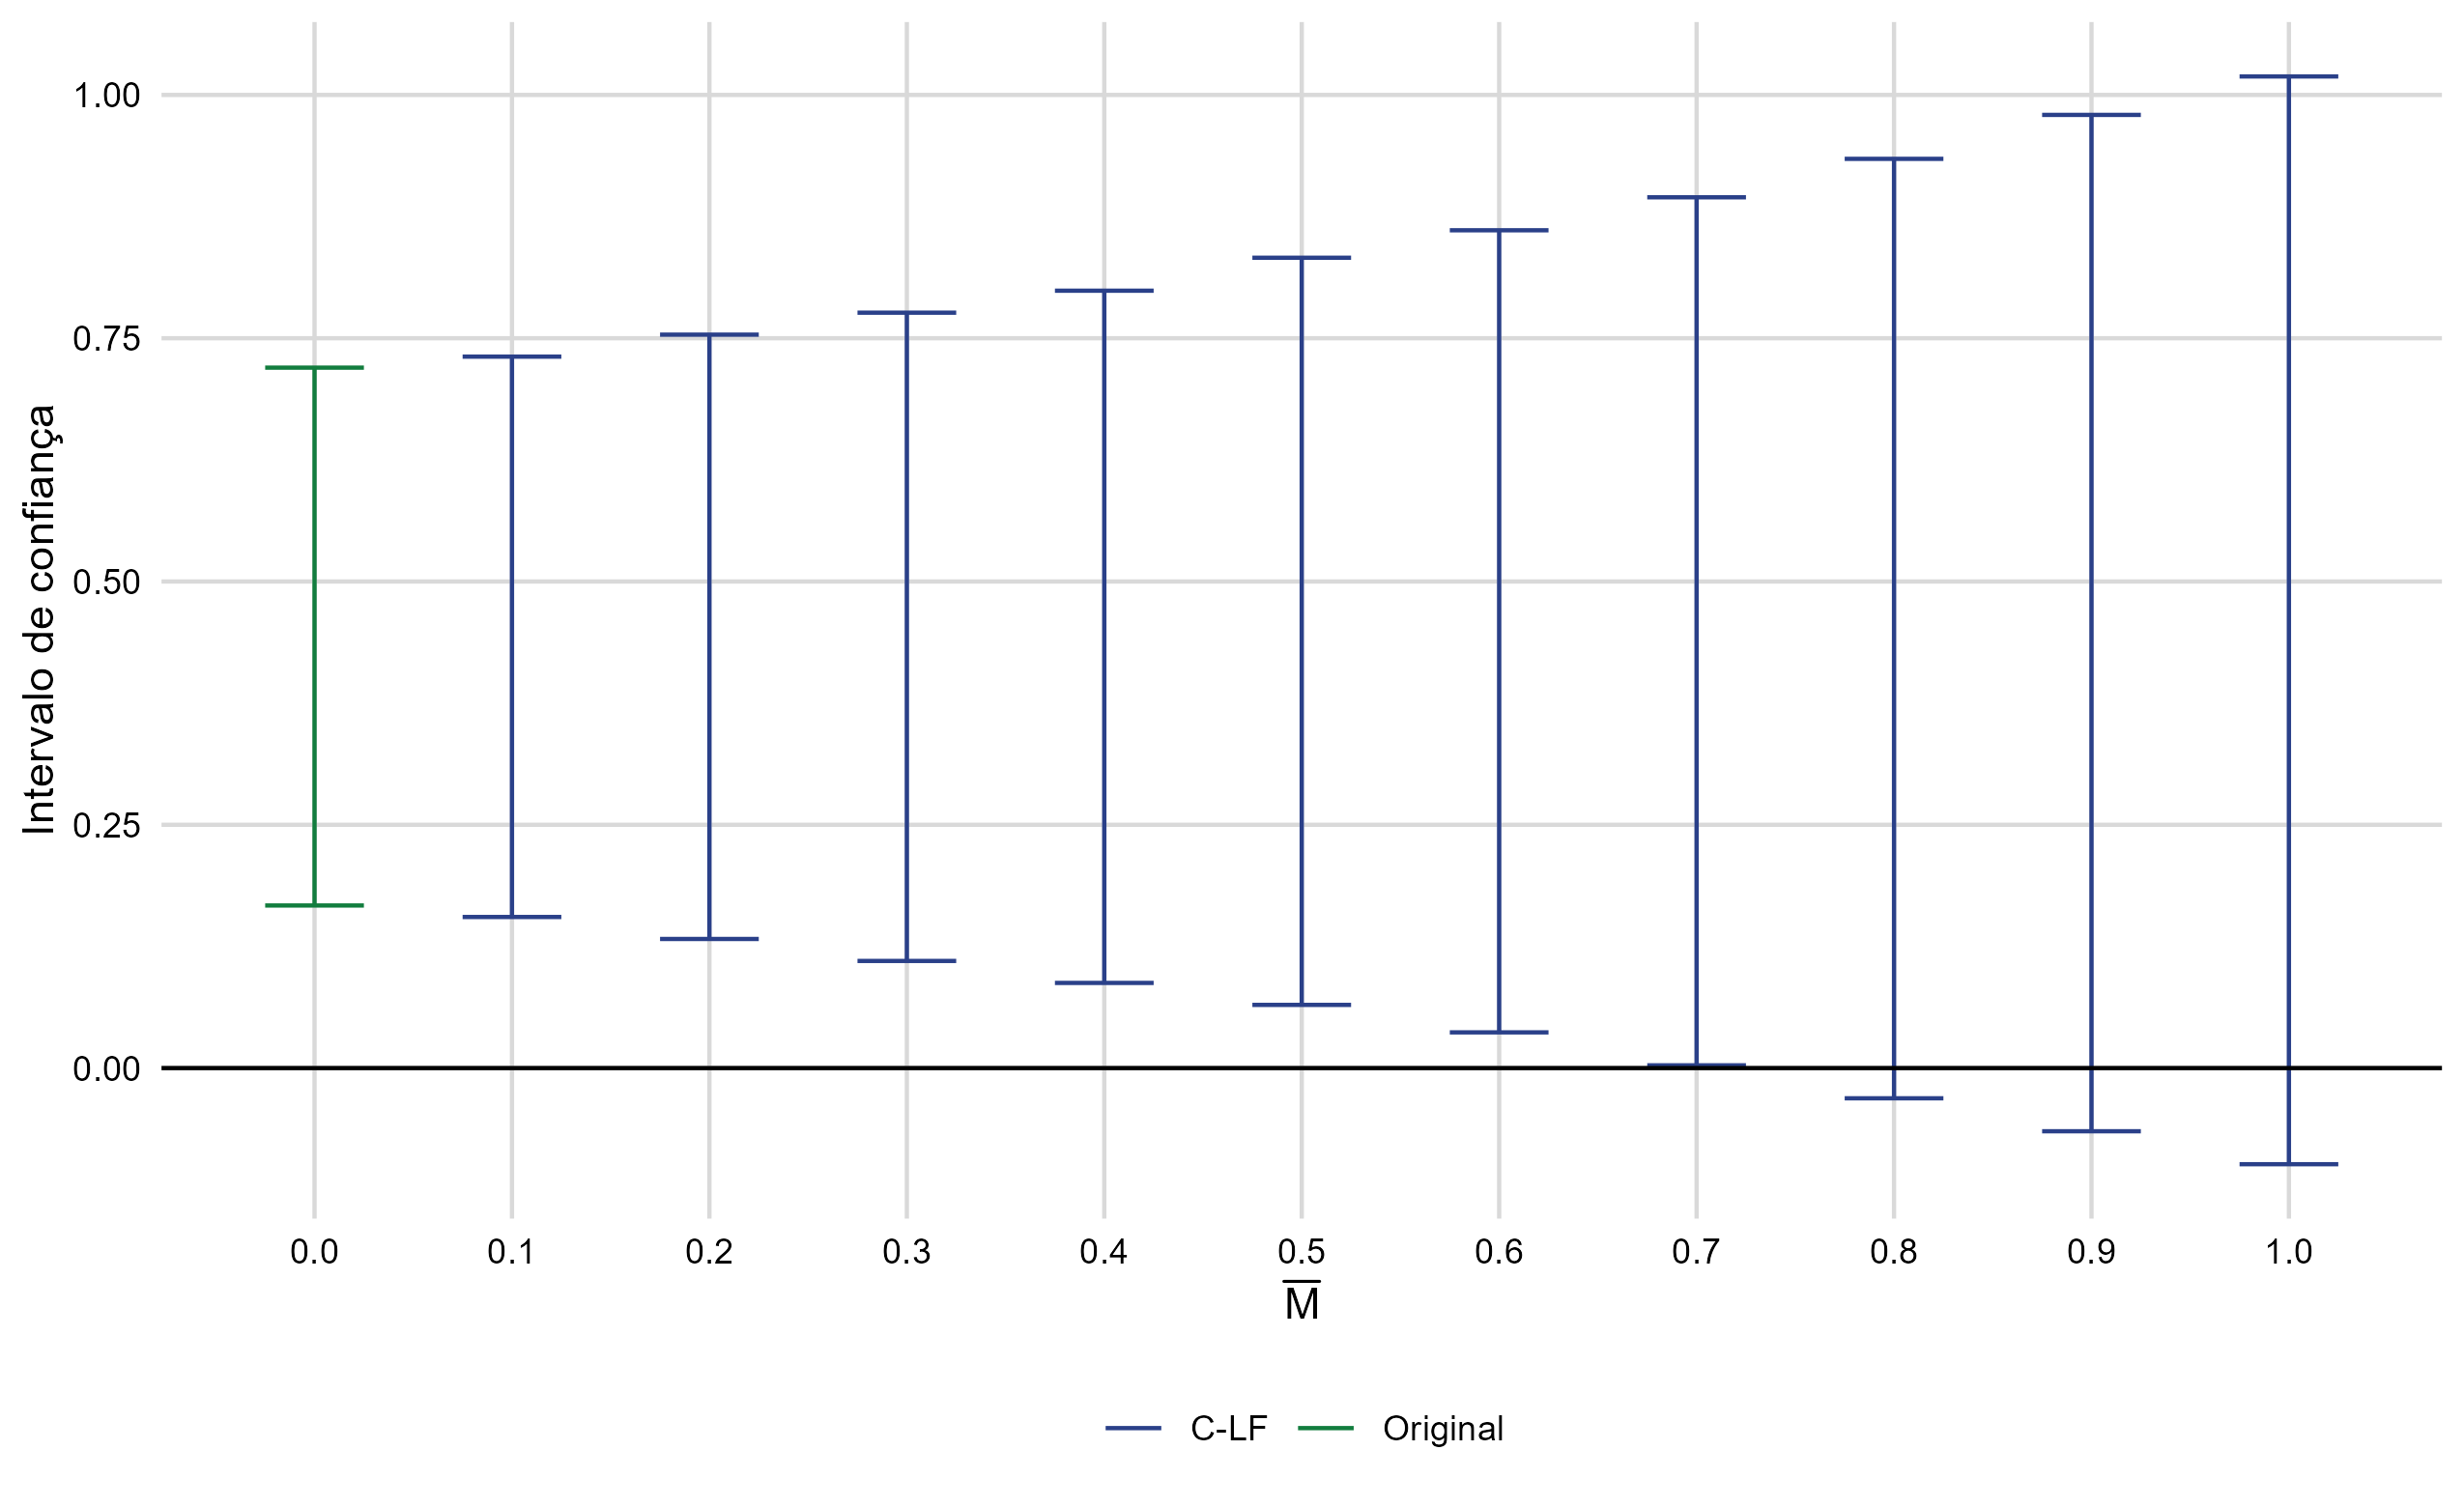
\includegraphics[width=0.96\textwidth]{HonestDiD - Log-massa-salarial.png}
\caption{HonestDiD: massa salarial}
\label{fig:honest_massa}
\figurenote{Intervalos de confiança robustos a desvios relativos de tendências paralelas. Verde:
intervalo original; azul: intervalo C-LF para cada $\bar M$.}
\end{figure}

\begin{figure}[p]
\centering
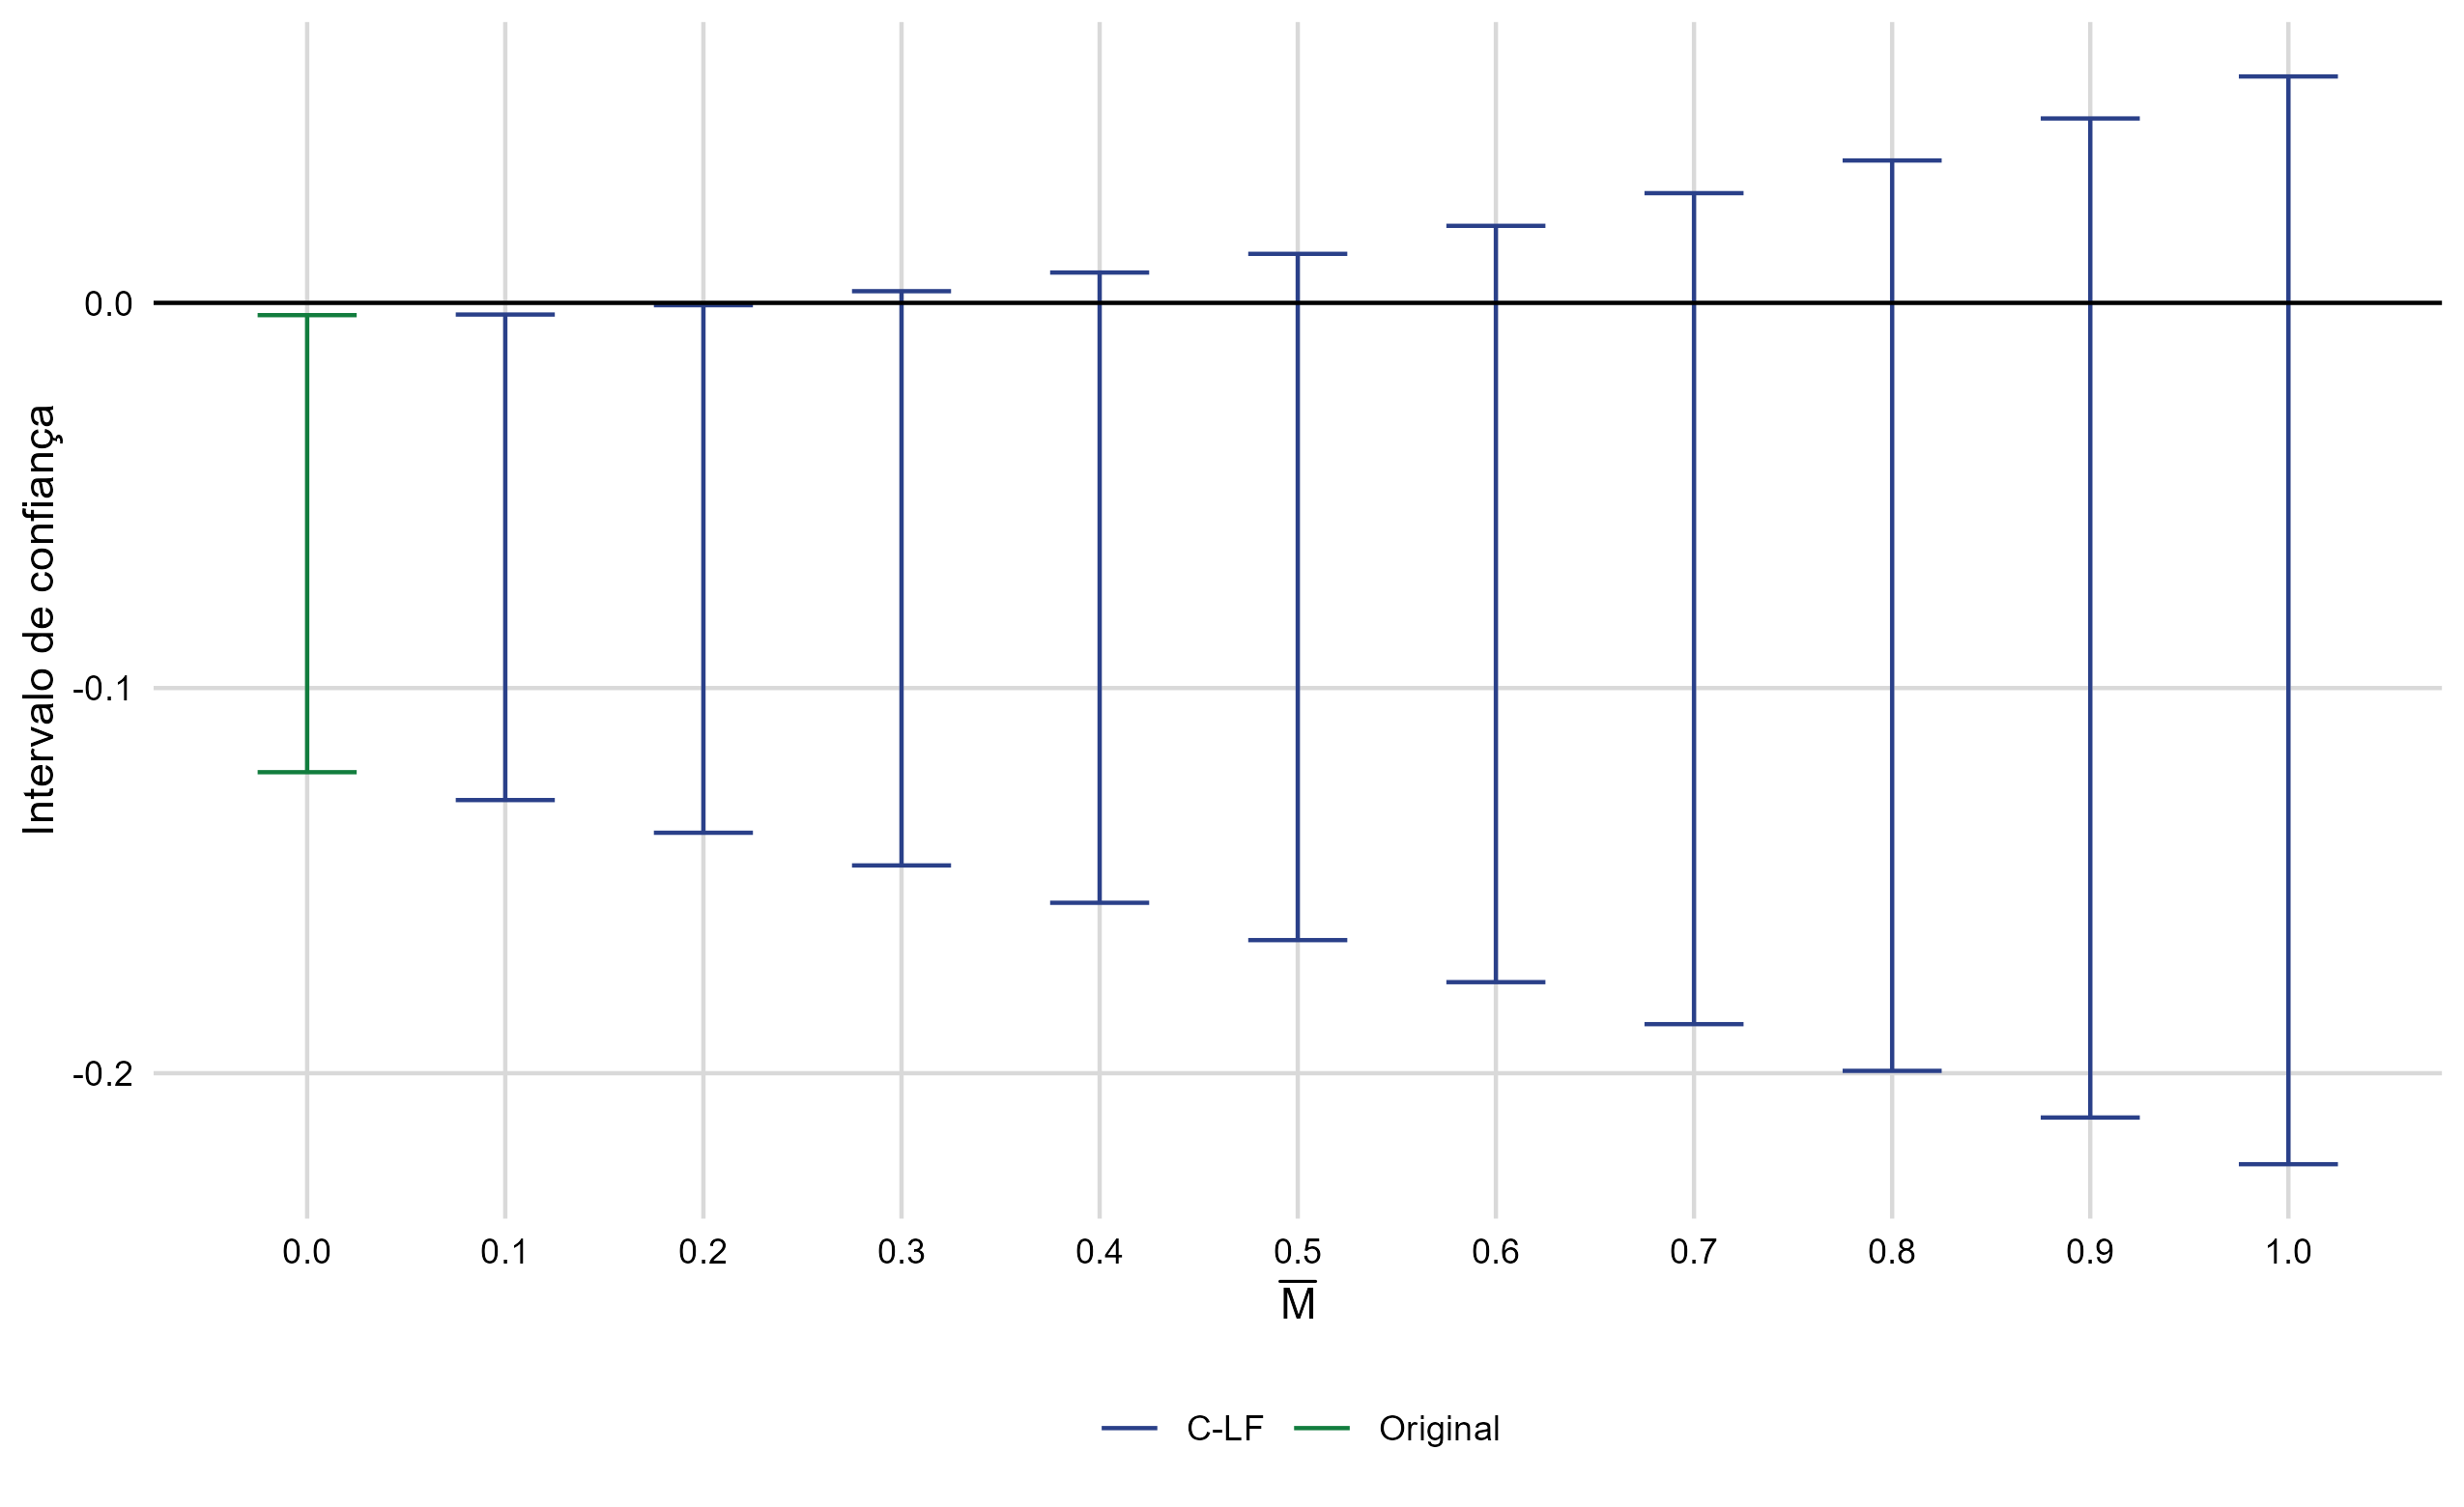
\includegraphics[width=0.96\textwidth]{HonestDiD - Log-salario-medio.png}
\caption{HonestDiD: salário médio}
\label{fig:honest_salario}
\figurenote{Intervalos de confiança robustos a desvios relativos de tendências paralelas. Verde:
intervalo original; azul: intervalo C-LF para cada $\bar M$.}
\end{figure}

\clearpage
\subsection{Conclusão das robustezes}

As checagens corroboram um efeito positivo do FUST sobre emprego no curto prazo: o sinal, a ordem
de grandeza e a dinâmica sobrevivem a mudanças de inferência, pareamento, estimador e desvios
consideráveis de tendências paralelas. A evidência para massa salarial também é positiva e
recorrente, porém mais sensível e menos precisa. Para salário médio, não há suporte para aumento;
algumas especificações sugerem redução no ano seguinte. Em conjunto, a conclusão mais defensável
é que o apoio FUST está associado à expansão do número de vínculos e da folha salarial das
empresas beneficiárias, enquanto os efeitos sobre remuneração por trabalhador permanecem
incertos.

\end{document}
